%\setcounter{chapter}{25}
\chapter{Transformers}\label{chapter:transformers}

%\textit{Draft chapter from Torralba, Isola, Freeman (this is a computer vision textbook, hence the emphasis on CNNs; note that transformers are also very related to GNNs)}

\section{Introduction}

\index{Transformers}{\bf Transformers} are a recent family of architectures that generalize and expand the ideas behind convolutional neural nets (CNNs). The term for this family of architectures was coined by \cite{vaswani2017attention}, where they were applied to language modeling. Our treatment in this chapter more closely follows the \textbf{vision transformers} (\textbf{ViTs}) that were introduced in \cite{dosovitskiy2020vit}.% but the general class includes many variations with a long history~\cite{XX,YY,ZZ}.

Like CNNs, transformers factorize the signal processing problem into stages that involve independent and identically processed chunks. However, they also include layers that mix information across the chunks, called \textbf{attention layers}, so that the full pipeline can model dependencies between the chunks. %However, the way they do this is slightly more complicated than just cutting up the input tensor into patches.
\marginnote{Transformers were originally introduced in the field of natural language processing, where they were used to model language, that is, sequences of characters and words. As a result, some texts present transformers as an alternative to recurrent neural nets (RNNs) for sequence modeling, but in fact transformer layers are \textit{parallel} processing machines, like convolutional layers, rather than sequential machines, like recurrent layers.}[-2.2cm]

%Transformers are also a special case of a more general architecture called ``graph neural networks,'' which we do not cover in this book.

%Transformers were introduced in \cite{vaswani2017attention} for natural language processing (NLP), although the technical components have a long history in the literature~\cite{XX,YY,ZZ}.

%Transformers can be understood as CNNs with additional layers -- which are called ``attention" layers -- inserted to mix information across across chunks.

\section{A Limitation of CNNs: Independence between Far Apart Patches}
CNNs are built around the idea of \textit{locality}: different local regions of an image can safely be processed independently. This is what allows us to use filters with small kernels. However, very often, there is global information that needs to be shared across all receptive fields in an image. Convolutional layers are not well-suited to \textit{globalizing} information since the only way they can do so is by either increasing the kernel size of their filters or stacking layers to increase the receptive field of neurons on deeper layers. \Fig{\ref{fig:transformers:CNN_limitations}} shows the inability of a shallow CNN to compare two input nodes ($x_1$ and $x_7$) that are spatially too far apart:

\begin{figure}
    \centerline{
        \begin{tikzpicture}
            %
            \def\Nnodes{7}
            \def\Nlayers{3}
            \def\layerheight{1.2}
            \def\neuronrad{0.1}
            \def\neuronstep{0.3}
            % draw nodes
            \foreach \y in {1,...,\Nlayers} {
                    \foreach \x in {1,...,\Nnodes} {
                            \draw [fill=white] (\neuronstep*\x,\y*\layerheight-\layerheight) circle (\neuronrad);
                        }
                }
            %
            \node [circle, draw, pattern=north east lines, inner sep=\neuronrad*0.7 cm, minimum size=\neuronrad, label=below:$x_1$] (myNode) at (\neuronstep,0) {};
            \node [circle, draw, pattern=north west lines, inner sep=\neuronrad*0.7 cm, minimum size=\neuronrad, label=below:$x_\Nnodes$] (myNode) at (\neuronstep*\Nnodes,0) {};
            %
            \foreach \x in {1,...,2} {
                    \draw [pattern=north east lines] (\neuronstep*\x,\layerheight) circle (\neuronrad);
                }
            \foreach \x in {1,...,3} {
                    \draw [pattern=north east lines] (\neuronstep*\x,\layerheight*2) circle (\neuronrad);
                }
            \foreach \x in {1,...,2} {
                    \draw [pattern=north west lines] (\neuronstep*\Nnodes-\neuronstep*\x+\neuronstep,\layerheight) circle (\neuronrad);
                }
            \foreach \x in {1,...,3} {
                    \draw [pattern=north west lines] (\neuronstep*\Nnodes-\neuronstep*\x+\neuronstep,\layerheight*2) circle (\neuronrad);
                }
            % draw edges
            \pgfmathtruncatemacro{\NlayersMinusOne}{\Nlayers - 1}
            \pgfmathtruncatemacro{\NNodesPlusOne}{\Nnodes + 1}
            \foreach \y in {1,...,\NlayersMinusOne} {
                    \foreach \x in {1,...,\Nnodes} {
                            \foreach \k in {-1,...,1} {
                                    \pgfmathtruncatemacro{\xk}{\x+\k}
                                    \ifnum \xk>0
                                        \ifnum \xk<\NNodesPlusOne
                                            \draw [thin, color=gray!33] [nn_edge] (\neuronstep*\x,\layerheight*\y+\neuronrad-\layerheight) -- (\neuronstep*\xk,\layerheight*\y-\neuronrad);
                                        \fi
                                    \fi
                                }
                        }
                }
            %
            \draw [thick] [nn_edge] (\neuronstep*1,\layerheight*1+\neuronrad-\layerheight) -- (\neuronstep*1,\layerheight*1-\neuronrad);
            \draw [thick] [nn_edge] (\neuronstep*1,\layerheight*1+\neuronrad-\layerheight) -- (\neuronstep*2,\layerheight*1-\neuronrad);
            \draw [thick] [nn_edge]         (\neuronstep*\Nnodes,\layerheight*1+\neuronrad-\layerheight) -- (\neuronstep*\Nnodes,\layerheight*1-\neuronrad);
            \draw [thick] [nn_edge]         (\neuronstep*\Nnodes,\layerheight*1+\neuronrad-\layerheight) -- (\neuronstep*\Nnodes-\neuronstep,\layerheight*1-\neuronrad);
            %
            \draw [thick] [nn_edge] (\neuronstep*1,\layerheight*2+\neuronrad-\layerheight) -- (\neuronstep*1,\layerheight*2-\neuronrad);
            \draw [thick] [nn_edge] (\neuronstep*1,\layerheight*2+\neuronrad-\layerheight) -- (\neuronstep*2,\layerheight*2-\neuronrad);
            \draw [thick] [nn_edge]         (\neuronstep*\Nnodes,\layerheight*2+\neuronrad-\layerheight) -- (\neuronstep*\Nnodes,\layerheight*2-\neuronrad);
            \draw [thick] [nn_edge]         (\neuronstep*\Nnodes,\layerheight*2+\neuronrad-\layerheight) -- (\neuronstep*\Nnodes-\neuronstep,\layerheight*2-\neuronrad);
            \foreach \k in {-1,...,1} {
                    \pgfmathtruncatemacro{\xk}{2+\k}
                    \draw [thick] [nn_edge] (\neuronstep*2,\layerheight*2+\neuronrad-\layerheight) -- (\neuronstep*\xk,\layerheight*2-\neuronrad);
                }
            \foreach \k in {-1,...,1} {
                    \pgfmathtruncatemacro{\xk}{\Nnodes-1+\k}
                    \draw [thick] [nn_edge] (\neuronstep*\Nnodes-\neuronstep,\layerheight*2+\neuronrad-\layerheight) -- (\neuronstep*\xk,\layerheight*2-\neuronrad);
                }
            %
            % \foreach \x in {1,...,3} {
            %     \draw [thick] [nn_edge] (\neuronstep*\x,\neuronrad) -- (\neuronstep*2,\layerheight-\neuronrad);
            % }
            % \foreach \x in {5,...,\Nnodes} {
            %     \draw [thick] [nn_edge] (\neuronstep*\x,\neuronrad) -- (\neuronstep*\Nnodes-\neuronstep,\layerheight-\neuronrad);
            % }
            %
            % \foreach \x in {2,...,4} {
            %     \draw [thick] [nn_edge] (\neuronstep*\x,\layerheight+\neuronrad) -- (\neuronstep*3,2*\layerheight-\neuronrad);
            % }
            % \pgfmathtruncatemacro{\NnodesMinusOne}{\Nnodes - 1}
            % \foreach \x in {4,...,\NnodesMinusOne} {
            %     \draw [thick] [nn_edge] (\neuronstep*\x,\layerheight+\neuronrad) -- (\neuronstep*\Nnodes-\neuronstep*2,2*\layerheight-\neuronrad);
            % }
        \end{tikzpicture}
    }
    \caption{Consider a 2-layer CNN with kernel size 3, tasked to compare $x_1$ and $x_7$. It can't do it: there are no neurons that are connected to both $x_1$ and $x_7$. Hatch marks indicate which neurons are connected to $x_1$ and $x_7$ respectively.}
    \label{fig:transformers:CNN_limitations}
\end{figure}
%\vspace{-0.5cm}

How can we efficiently pass messages across large spatial distances? We already have seen one option: just use a fully connected layer, so that every output neuron after this layer takes input from every neuron on the layer before. However, fully connected layers have a ton of parameters ($N^2$ if their input and output are $N$-dimensional vectors), and it can take an exorbitant amount of time and data to fit all those parameters. Can we come up with a more efficient strategy?

%[Example image with different attention maps.]

\section{The Idea of Attention}
Attention is a strategy for processing global information efficiently, focusing just on the parts of the signal that are most salient to the task at hand. The idea can be motivated by attention in human perception. When we look at a scene, our eyes flick around and we attend to certain elements that stand out, rather than taking in the whole scene at once~\cite{wolfe2000visual}. If we are asked a question about the color of a car in the scene, we will move our eyes to look at the car, rather than just staring passively. Can we give neural nets the same ability?

In neural nets, attention follows the same intuitive idea. A set of neurons on layer $l+1$ may \textit{attend} to a set of neurons on layer $l$, in order to decide what their response should be. If we ``ask'' that set of neurons to report the color of any cars in the input image, then they should direct their attention to the neurons on the previous layer that represent the color of the car. We will soon see how this is done, in full detail, but first we need to introduce a new data structure and a new way of thinking about neural processing.

\section{A New Data Type: Tokens}
We discussed that the main data structures in deep learning are different kinds of groups of neurons: channels, tensors, batches, and so on. Now we will introduce another fundamental data structure, \index{Tokens}{\bf tokens}. A token is another kind of group of neurons, but there are particular ways we will operate over tokens that are different from how we operated over channels, batches, and the other groupings we saw before. Specifically,  we will think of tokens as \textit{encapsulated} groups of information; we will define operators over tokens, and these operators will be our only interface for accessing and modifying the internal contents of tokens. From a programming languages perspective, you can think of tokens as a new data \textit{type}.

In this chapter we will only consider tokens whose internal content is a vector of neurons. A single token will therefore be represented by a column vector $\mathbf{t} \in \mathbb{R}^{d \times 1}$, which is also sometimes called the token's \index{Code vector}\textbf{code vector}.

%Therefore, we should think of tokens as a new data \textit{type}, with specific syntax and semantics. 

%\marginnote{Vectors of neurons are given different names and connotations in different contexts. In the context of representation learning, they are more commonly called ``embeddings".}[-1.0cm]

%At first it might not seem like we need a new term here, but the reason it's useful is because ``tokens" come with connotations about how we will use them. In particular, we will think of tokens as encapsulated groups of information; we will define operators over tokens, and these operators will be our only interface for accessing and modifying the internal contents of tokens.\marginnote{With this way of thinking, it's easy to imagine tokens that are any kind of structured group, rather than just being vectors of neurons. We just need to define how basic operators, like summation, operate over these groups (and, ideally, in a differentiable manner).}[-1.2cm] 



\subsection{Tokenizing Data}
%The way to think about tokens is as discrete bundles of information about some entity. 
The first step to working with tokens is to \textit{tokenize} the raw input data. Once we have done this, all subsequent layers will operate over tokens, until the output layer, which will make some decision or prediction as a function of the final set of tokens. How can we tokenize an input image? Well, how did we ``neuronize'' an image for processing in a vanilla neural net? We simply represented each \textit{pixel} in the image with a neuron (or three neurons, if it's a color image). To tokenize an image, we may simply represent each \textit{patch of pixels} in the image with a token. The token vector is the vectorized patch (stacking the three color channels one after the other), or a lower-dimensional projection of the vectorized patch.
%created a tensor of neurons $\mathbf{x} \in \mathbb{R}^{N \times M \times C}$ whose values took on the color values of the pixels in the image. To tokenize an image, a common approach is to simply vectorize each \textit{patch} of pixels in the image, listing the color value of each pixel in sequential order. 
With each patch represented by a token, the full image corresponds to an array of tokens. \Fig{\ref{fig:transformers:tokenization}} shows what it looks like to tokenize a safari image in this way.


\begin{figure}[h!]
    %\newgeometry{papersize={8in,9in},bottom=3pc,top=5pc,left=6pc,right=12pc,headsep=2pc,marginparwidth=8pc, marginparsep=1pc, textwidth=30pc, textheight=45pc}
    \centerline{
        %\resizebox{\columnwidth}{!}{
        \begin{tikzpicture}
            \draw (0, -1.25) node[inner sep=0] {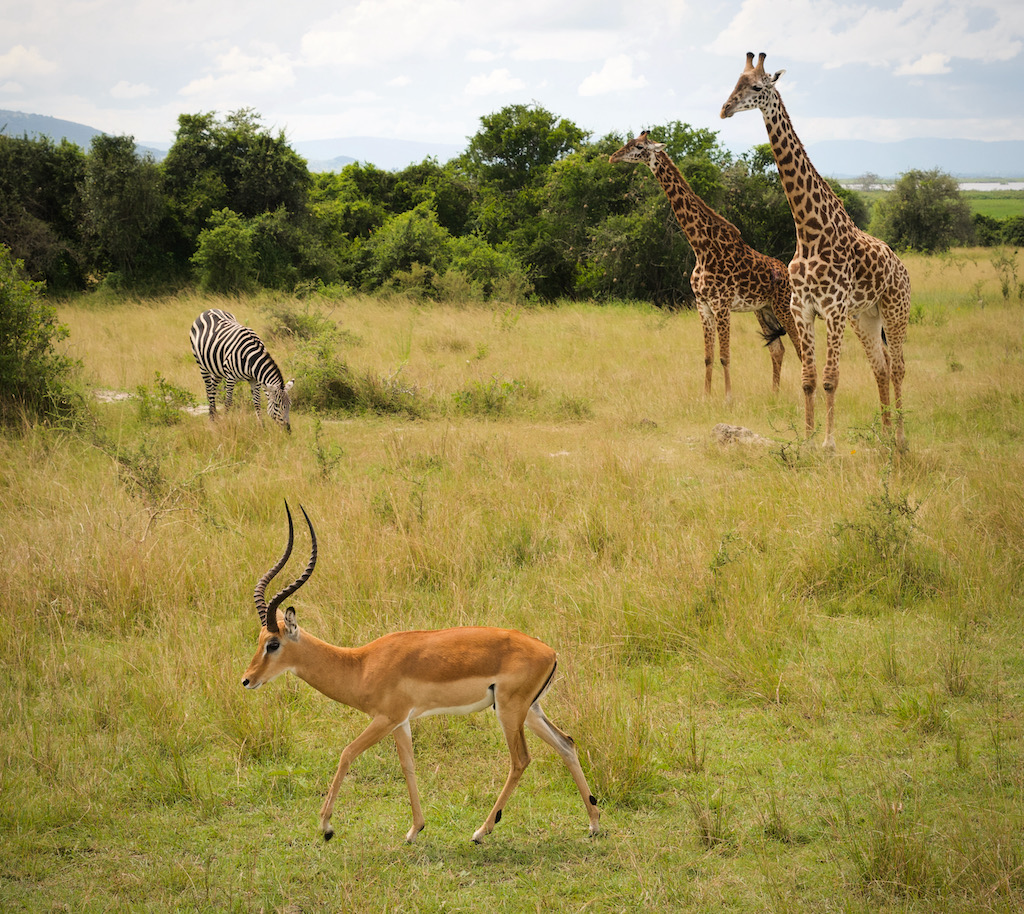
\includegraphics[width=0.31\linewidth]{./figures/transformers/zebras_giraffes_impalas/zebras_giraffes_impalas.jpeg}};
            \draw (-2,1.8) node[inner sep=0] {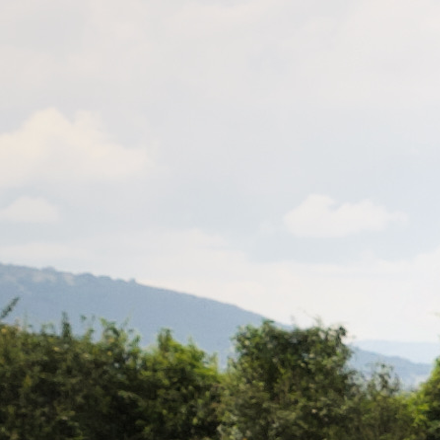
\includegraphics[width=0.05\linewidth]{./figures/transformers/zebras_giraffes_impalas/patch_0_0.png}};
            \draw (-1,1.8) node[inner sep=0] {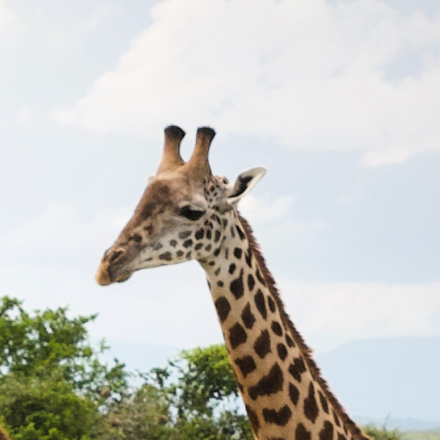
\includegraphics[width=0.05\linewidth]{./figures/transformers/zebras_giraffes_impalas/patch_4_0.png}};
            \draw (1,1.8) node[inner sep=0] {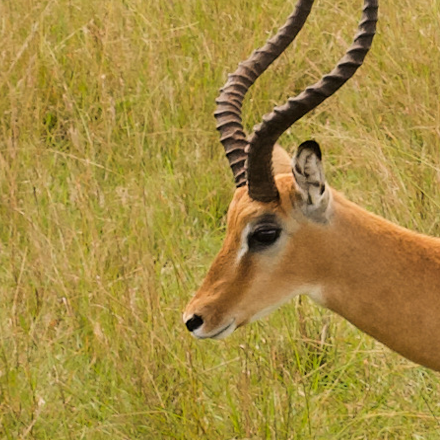
\includegraphics[width=0.05\linewidth]{./figures/transformers/zebras_giraffes_impalas/patch_1_3.png}};
            \draw (2,1.8) node[inner sep=0] {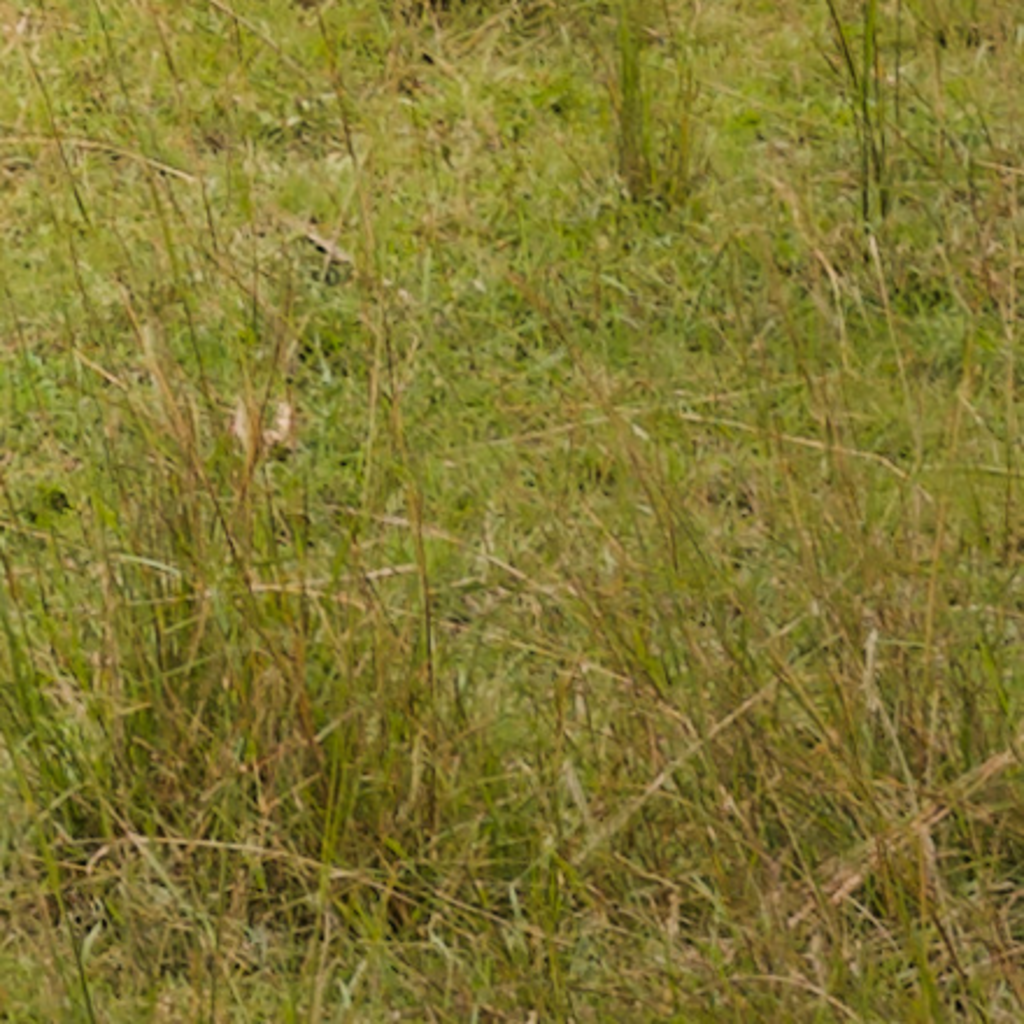
\includegraphics[width=0.05\linewidth]{./figures/transformers/zebras_giraffes_impalas/patch_5_4.png}};
            %
            \def\neuronrad{0.3}
            %
            \draw [nn_edge, thick] (0,0.9) -- (0,1.4);
            \draw (0.5,1.05) node {$\small{\texttt{crop}}$};
            \draw [nn_edge, thick] (-2,2.3) -- (-2,2.8);
            \draw [nn_edge, thick] (-1,2.3) -- (-1,2.8);
            \draw [nn_edge, thick] (1,2.3) -- (1,2.8);
            \draw [nn_edge, thick] (2,2.3) -- (2,2.8);
            \draw (2.85, 2.45) node {$\mathbf{W}_{\texttt{tokenize}}$};
            \draw [fill=white] (-2.075,2.8) rectangle ++(\neuronrad/2,\neuronrad*2);
            \draw [fill=white] (-1.075,2.8) rectangle ++(\neuronrad/2,\neuronrad*2);
            \draw [fill=white] (0.925,2.8) rectangle ++(\neuronrad/2,\neuronrad*2);
            \draw [fill=white] (1.925,2.8) rectangle ++(\neuronrad/2,\neuronrad*2);
            \draw (2.75, 3.1) node {$\Big\} \: \mathbf{t} \in \mathbb{R}^d$};
            %
            \draw (0, 1.8) node {$\ldots$};
            \draw (-3.55, 3.075) node {tokens}; \draw (-2.75,2.8) -- (-2.75,3.35);
            \draw (-3.55, 1.8) node {patches}; \draw (-2.75,1.4) -- (-2.75,2.2);
            \draw (-3.55, -1.25) node {input}; \draw (-2.75,-3.3) -- (-2.75,0.8);
        \end{tikzpicture}
    }
    %\restoregeometry
    \caption{Tokenization: converting an image to a set of vectors. $\mathbf{W}_{\texttt{tokenize}}$ is a learnable linear projection from the dimensionality of the vectorized crops to $d$ dimensions. This is just one of many possible ways to tokenize an image.}
    \label{fig:transformers:tokenization}
\end{figure}

%In language modeling, a token might represent a word, so that a sequence of tokens is a sentence. In computer vision, a token may correspond to an image patch, so that an array of tokens represents an image.

\subsection{Data Structures and Notation for Working with Tokens}

A sequence of tokens will be denoted by a matrix $\mathbf{T} \in \mathbb{R}^{N \times d}$, in which each token in the sequence, $\mathbf{t}_1, \ldots, \mathbf{t}_N$, is transposed to become a row of the matrix:
\begin{equation}
    \mathbf{T} =
    \begin{bmatrix}
        \mathbf{t}_1^\transpose \\
        \vdots                  \\
        \mathbf{t}_N^\transpose \\
    \end{bmatrix}
\end{equation}
\marginnote{As we will see, transformers are invariant to permutations of the input sequence, so, as far as transformers are concerned, groups of tokens should be thought of a \textit{sets} rather than ordered sequences.}[-0.4cm]

Graphically, $\mathbf{T}$ is constructed from $\mathbf{t}_1, \ldots, \mathbf{t}_N$ like this (\fig{\ref{fig:transformers:T_notation}}):
\begin{figure}
    \centerline{
        \begin{tikzpicture}
            % token sequence
            \def\Nx{4}
            \def\Ny{3}
            \def\cellwidth{0.25}
            \def\rowmargin{0.2}
            \def\neuronrad{0.3}
            % draw individual tokens as token symbols
            \foreach \x in {1,...,\Ny} {
                    \draw [fill=white] (\cellwidth*-8.5-3+\x*1.5*\neuronrad,-0.5) rectangle ++(\neuronrad/2,\neuronrad*2);
                    \draw (\cellwidth*-8.5-3+\x*1.5*\neuronrad+\neuronrad/4,-0.5-0.25) node {$\mathbf{t}_{\x}$};
                }
            % draw arrow from token sequence to token rows
            \draw [thick, dashed, nn_edge] (\cellwidth*-8.5-3.2+\Nx*1.5*\neuronrad+\neuronrad/4,-\rowmargin*2+\rowmargin*1.5+\cellwidth*1.5) .. controls (\cellwidth*-11, -\rowmargin*1+\rowmargin*1.5+0.25+\cellwidth*1.5) .. (\cellwidth*-7.8, -\rowmargin*2+\rowmargin*1.5+\cellwidth*1.5)
            node[midway, above] {transpose};
            % draw individual tokens as rows
            \foreach \x in {1,...,\Nx} {
                    \foreach \y in {1,...,\Ny} {
                            \draw [fill=white] (\cellwidth*\x-\cellwidth*5.5-\cellwidth,-\rowmargin*\y+\rowmargin*1.5-\cellwidth*\y+\cellwidth) rectangle ++(\cellwidth,\cellwidth);
                        }
                }
            \draw (\cellwidth*-6.5, -\rowmargin*1+\rowmargin*1.5-\cellwidth*1+\cellwidth*1.5) node {$\mathbf{t}_1^\transpose$};
            \draw (\cellwidth*-6.5, -\rowmargin*2+\rowmargin*1.5-\cellwidth*2+\cellwidth*1.5) node {$\mathbf{t}_2^\transpose$};
            \draw (\cellwidth*-6.5, -\rowmargin*3+\rowmargin*1.5-\cellwidth*3+\cellwidth*1.5) node {$\mathbf{t}_3^\transpose$};
            % draw arrows from individual tokens to T
            \draw [thick, nn_edge] (-\cellwidth*1.5,             \rowmargin*0.5+\cellwidth*0.5) .. controls (\cellwidth, \rowmargin*0.5+\cellwidth*0.5) and (\cellwidth, \cellwidth*0.5-\rowmargin*0.5) ..  (\cellwidth*3.5,\cellwidth*0.5-\rowmargin*0.5);
            %
            \draw [thick, nn_edge] (-\cellwidth*1.5,             -\rowmargin*0.5-\cellwidth*0.5) -- (\cellwidth*3.5,-\rowmargin*0.5-\cellwidth*0.5);
            %
            \draw [thick, nn_edge] (-\cellwidth*1.5,             -\rowmargin*1.5-\cellwidth*1.5) .. controls (\cellwidth, -\rowmargin*1.5-\cellwidth*1.5) and (\cellwidth, -\cellwidth*1.5-\rowmargin*0.5) ..  (\cellwidth*3.5,-\cellwidth*1.5-\rowmargin*0.5);
            %
            % draw T
            \foreach \x in {1,...,\Nx} {
                    \foreach \y in {1,...,\Ny} {
                            \draw [fill=white] (\cellwidth*\x+\cellwidth*3.5-\cellwidth,-\cellwidth*\y+\cellwidth-\rowmargin*0.5) rectangle ++(\cellwidth,\cellwidth);
                        }
                }
            \draw (\cellwidth*1.5+\cellwidth*4, \cellwidth*2-\rowmargin*0.5) node {$\mathbf{T}$};
            \draw[decorate,decoration={brace, amplitude=5pt, mirror, angle=180}] (\cellwidth*3.5,-\cellwidth*2-0.2) -- (\cellwidth*7.5,-\cellwidth*2-0.2);
            \node[below] at (\cellwidth*5.5,-\cellwidth*2-0.3) {$d$ channels};
            \draw[decorate,decoration={brace,amplitude=5pt, angle=90}] (\cellwidth*7.5+0.1,\cellwidth-0.1) -- (\cellwidth*7.5+0.1,-\cellwidth*2-0.1);
            \node[right, rotate=90] at (\cellwidth*7.5+0.5,-\cellwidth*4) {$N$ tokens};
        \end{tikzpicture}
    }
    \caption{In this chapter, we will represent a set of tokens as a matrix whose rows are the token vectors.}
    \label{fig:transformers:T_notation}
\end{figure}
\vspace{-0.4cm}

The idea of this notation is that \textit{tokens are to transformers as neurons are to neural nets}. Neural net layers operate over arrays of neurons; for example, an MLP takes as input a column vector $\mathbf{x}$, whose rows are scalar neurons. Transformers operate over arrays of tokens. A matrix $\mathbf{T}$ is just a convenient representation of 1D array of vector-value tokens.
% consider figure here showing 1D array of neurons vs 1D array of tokens.

%; the code for a token $t$ will be labeled as $t.\mathbf{z}$.
\marginnote{Although we are only considering vector-valued tokens in this chapter, it's easy to imagine tokens that are any kind of structured group. We just need to define how basic operators, like summation, operate over these groups (and, ideally, in a differentiable manner).}[-1.8cm]

Transformers consist of two main operations over tokens: (1) \textit{mixing} tokens via a weighted sum, and (2) \textit{modifying} each individual token via a nonlinear transformation. These operations are analogous to the two workhorses of regular neural nets: the linear layer and the pointwise nonlinearity. %Before we get to that, though, how do we turn data into tokens in the first place?

\subsection{Mixing Tokens}
Once we have converted our data to tokens, we now need to define operations for transforming these tokens and eventually making decisions based on them. The first operation we will define is how to take a \textit{linear combination of tokens}.

A linear combination of tokens is not the same as a fully connected layer in a neural net. Instead of taking a weighted sum of scalar neurons, it takes a weighted sum of vector-valued tokens (\fig{\ref{fig:transformers:lin_bomb_neurons_vs_tokens}}): %You can think of this operation as a linear transformation with block structure.
% Let $a$ and $b$ be two tokens:
% \begin{align}
%     a &= [a_1, \ldots, a_n]\\
%     b &= [b_1, \ldots, b_n]
% \end{align}
% Then we define the $+$ operator over tokens as an elementwise sum:
% \begin{align}
%     a + b \equiv [a_1 + b_1, \ldots, a_n + b_n]
% \end{align}
% Multiplication of a token $a$ with a scalar $w$ is defined as:
% \begin{align}
%     wa \equiv [wa_1, \ldots, wa_n]
% \end{align}
%Here, capital $\mathbf{X}$ is a matrix with each column being a token vector. You can think of $\mathbf{X}$ as being either a vector of tokens (a vector of vectors) or as a matrix of neurons (scalars). In the following sections, we will generally think of $\mathbf{X}$ as a vector, so that token operations become analogous to neural operations, just at a group level.
% \begin{figure}[h]
%     \centering
%     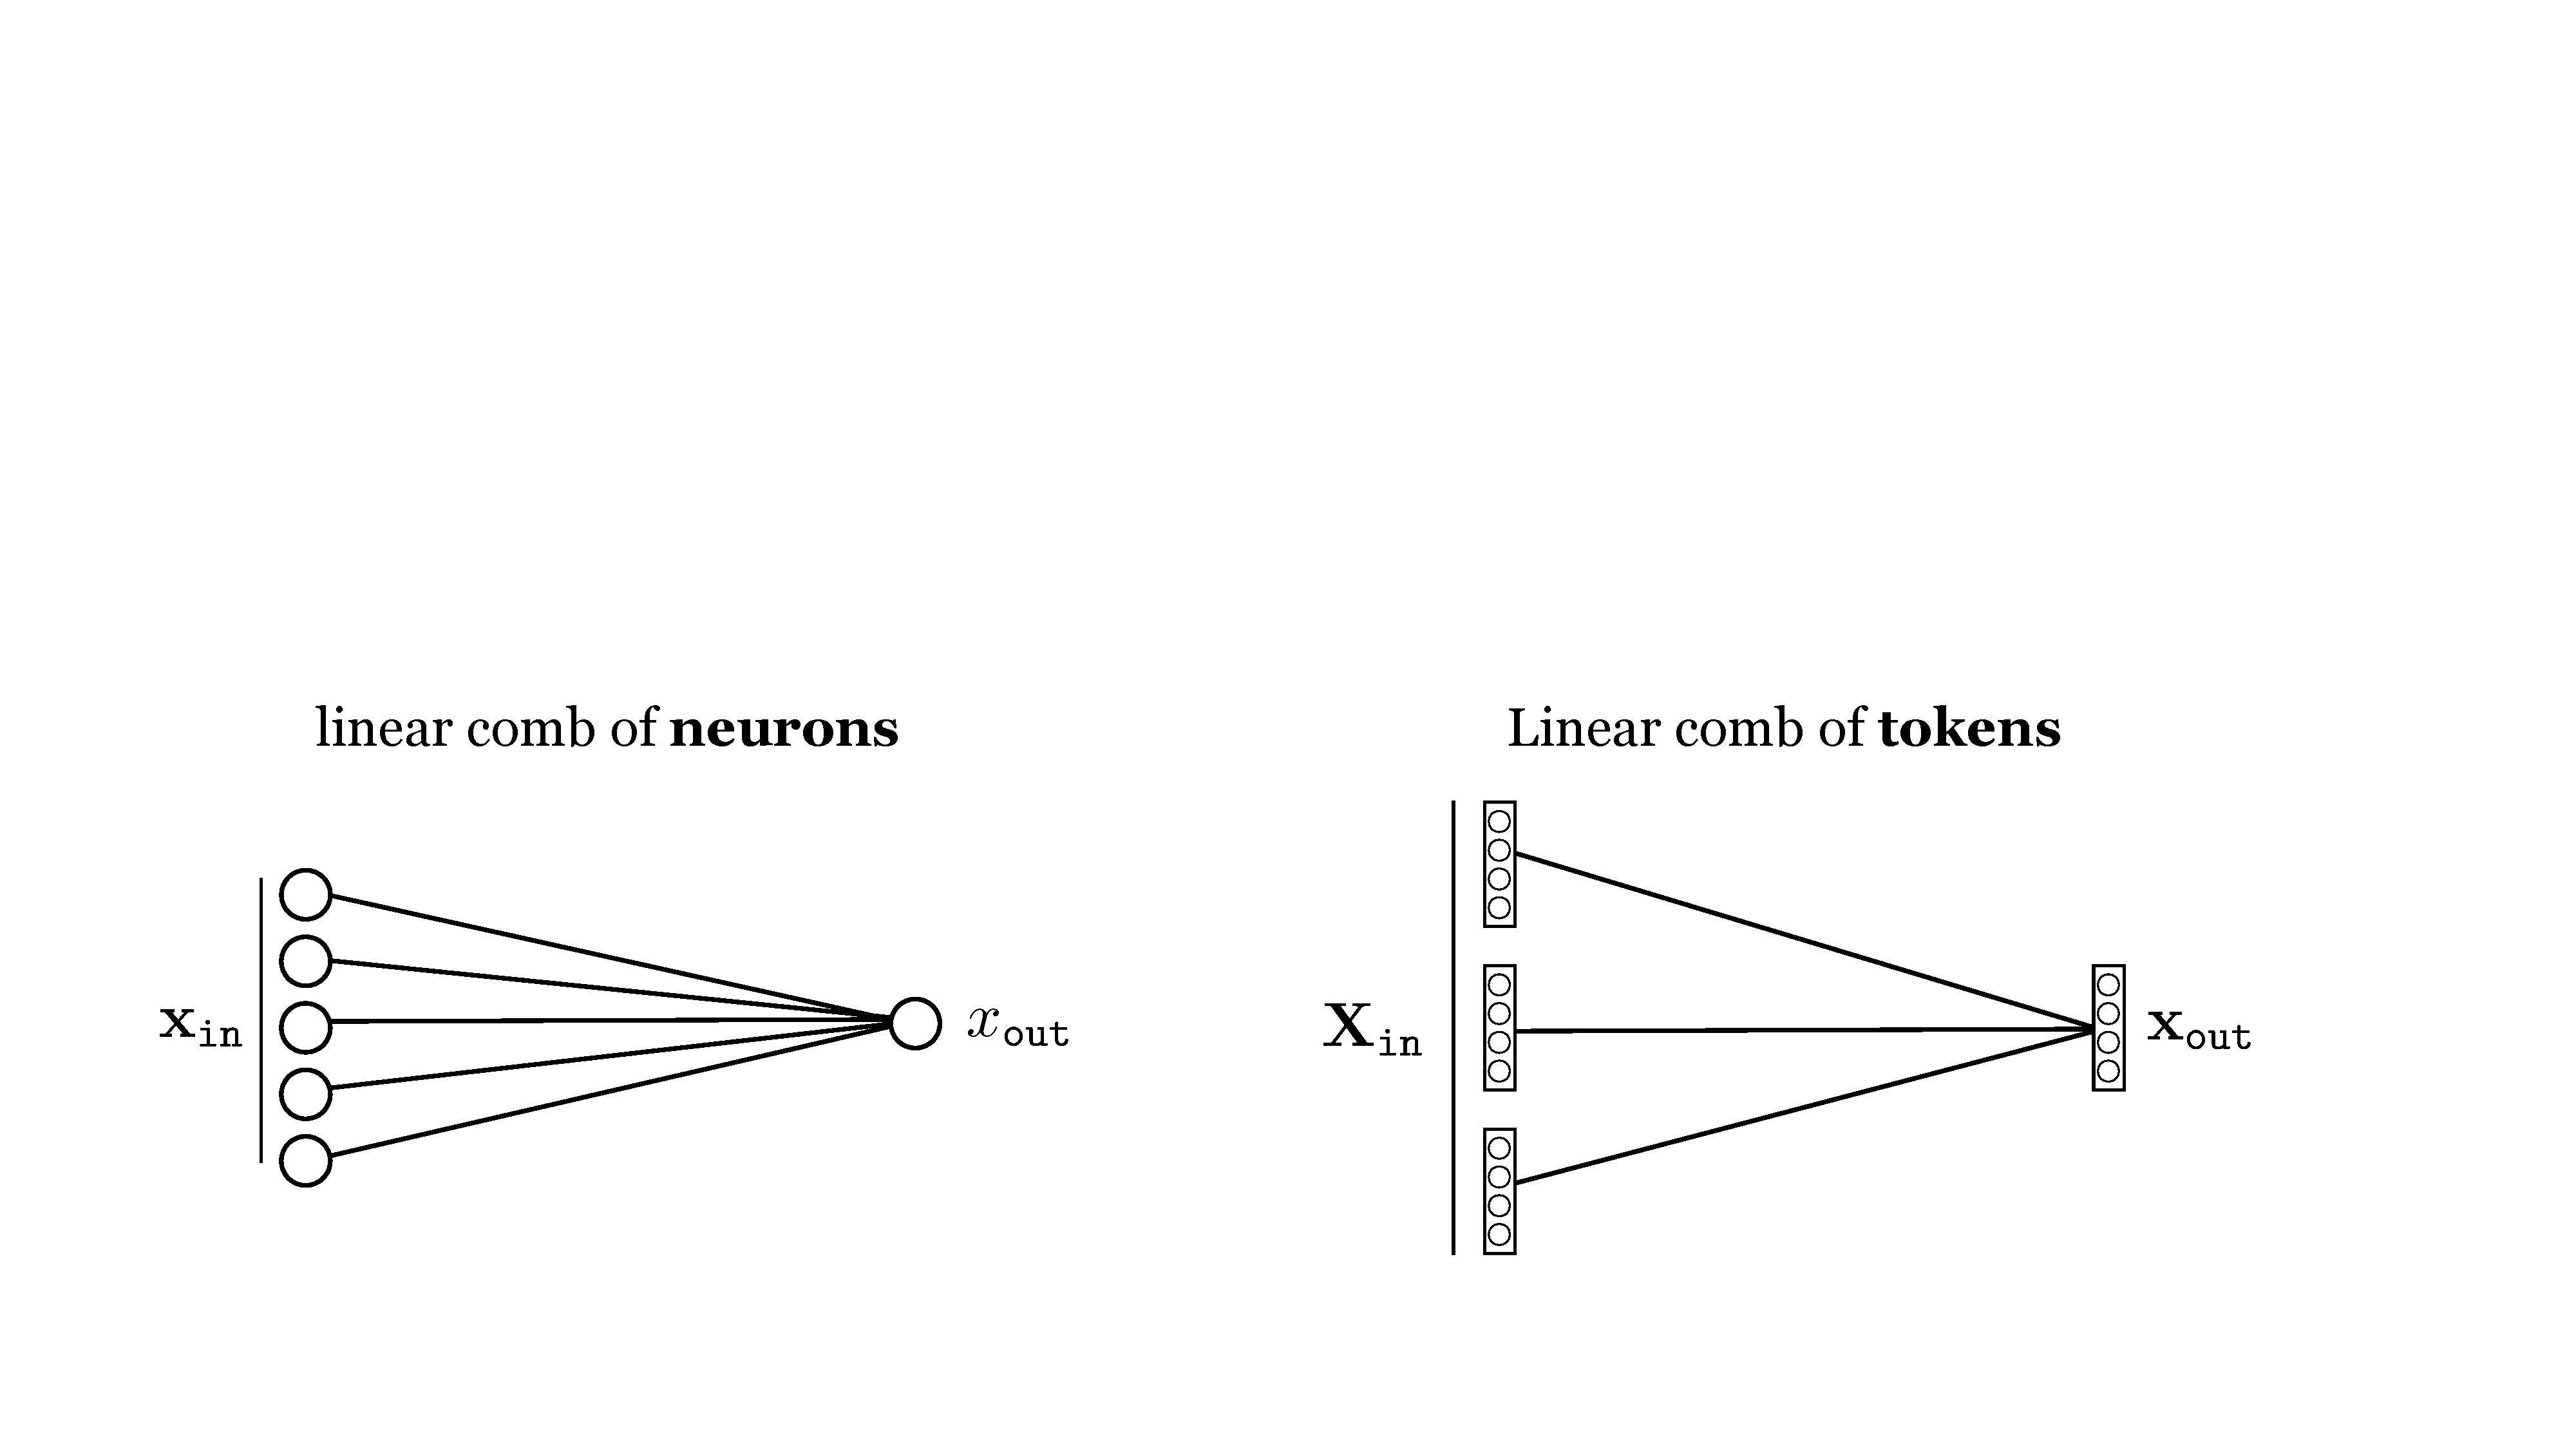
\includegraphics[width=0.9\linewidth]{./figures/transformers/lin_comb_neurons_vs_tokens.pdf}
%     \label{fig:transformers:lin_comb_neurons_vs_tokens}
%     \vspace{-0.4cm}
% \end{figure}
\begin{figure}[h]
    \centerline{
        \begin{minipage}{.49\linewidth}
            \centering
            \begin{tikzpicture}
                %
                \def\Nnodes{3}
                \def\layerheight{1.2}
                \def\neuronrad{0.1}
                \def\neuronstep{0.7}
                \draw [fill=gray!10] (\neuronstep,0) circle (\neuronrad);
                \draw [fill=gray!100] (\neuronstep*2,0) circle (\neuronrad);
                \draw [fill=gray!50] (\neuronstep*3,0) circle (\neuronrad);

                \draw [fill=gray!20] (\neuronstep*2,\layerheight) circle (\neuronrad);
                \foreach \x in {1,...,\Nnodes} {
                        \draw [thick] [nn_edge] (\neuronstep*\x,\neuronrad) -- (\neuronstep*2,\layerheight-\neuronrad);
                    }
                %
                \draw (\neuronstep*2,1.8*\layerheight) node {\textbf{Linear combination of neurons}};
                \draw (-\neuronstep,0) node {$\xin$};
                \draw (-\neuronstep,\layerheight) node {$x_{\texttt{out}}$};
                %
                \draw (\neuronstep*1,-0.3) node {$x_1$};
                \draw (\neuronstep*2,-0.3) node {$x_2$};
                \draw (\neuronstep*3,-0.3) node {$x_3$};
                \draw (\neuronstep*1+0.05,\layerheight*0.5) node {$w_1$};
                \draw (\neuronstep*2-0.22,\layerheight*0.3) node {$w_2$};
                \draw (\neuronstep*3-0.37,\layerheight*0.25) node {$w_3$};
                \draw (\neuronstep*2,-\layerheight*0.8) node {$x_{\texttt{out}} = w_1x_1 + w_2x_2 + w_3x_3$};
            \end{tikzpicture}
        \end{minipage}
        \begin{minipage}{.49\linewidth}
            \centering
            \begin{tikzpicture}
                %
                \def\Nnodes{3}
                \def\layerheight{1.2}
                \def\neuronrad{0.3}
                \def\neuronstep{0.7}
                \foreach \x in {1,...,\Nnodes} {
                        \draw (\neuronstep*\x-\neuronrad/4,(0-\neuronrad) rectangle ++(\neuronrad/2,\neuronrad*2);
                    }
                \draw [fill=gray!10] (\neuronstep,\neuronrad*2*0.25-\neuronrad-\neuronrad*0.25) circle (\neuronrad*0.25);
                \draw [fill=gray!25] (\neuronstep,\neuronrad*2*0.25*2-\neuronrad-\neuronrad*0.25) circle (\neuronrad*0.25);
                \draw [fill=gray!100] (\neuronstep,\neuronrad*2*0.25*3-\neuronrad-\neuronrad*0.25) circle (\neuronrad*0.25);
                \draw [fill=gray!50] (\neuronstep,\neuronrad*2*0.25*4-\neuronrad-\neuronrad*0.25) circle (\neuronrad*0.25);

                \draw [fill=gray!80] (\neuronstep*2,\neuronrad*2*0.25-\neuronrad-\neuronrad*0.25) circle (\neuronrad*0.25);
                \draw [fill=gray!110] (\neuronstep*2,\neuronrad*2*0.25*2-\neuronrad-\neuronrad*0.25) circle (\neuronrad*0.25);
                \draw [fill=gray!40] (\neuronstep*2,\neuronrad*2*0.25*3-\neuronrad-\neuronrad*0.25) circle (\neuronrad*0.25);
                \draw [fill=gray!10] (\neuronstep*2,\neuronrad*2*0.25*4-\neuronrad-\neuronrad*0.25) circle (\neuronrad*0.25);

                \draw [fill=gray!30] (\neuronstep*3,\neuronrad*2*0.25-\neuronrad-\neuronrad*0.25) circle (\neuronrad*0.25);
                \draw [fill=gray!60] (\neuronstep*3,\neuronrad*2*0.25*2-\neuronrad-\neuronrad*0.25) circle (\neuronrad*0.25);
                \draw [fill=gray!10] (\neuronstep*3,\neuronrad*2*0.25*3-\neuronrad-\neuronrad*0.25) circle (\neuronrad*0.25);
                \draw [fill=gray!120] (\neuronstep*3,\neuronrad*2*0.25*4-\neuronrad-\neuronrad*0.25) circle (\neuronrad*0.25);

                \draw (\neuronstep*2-\neuronrad/4,(\layerheight-\neuronrad) rectangle ++(\neuronrad/2,\neuronrad*2);

                \draw [fill=gray!40] (\neuronstep*2,\layerheight+\neuronrad*2*0.25-\neuronrad-\neuronrad*0.25) circle (\neuronrad*0.25);
                \draw [fill=gray!125] (\neuronstep*2,\layerheight+\neuronrad*2*0.25*2-\neuronrad-\neuronrad*0.25) circle (\neuronrad*0.25);
                \draw [fill=gray!50] (\neuronstep*2,\layerheight+\neuronrad*2*0.25*3-\neuronrad-\neuronrad*0.25) circle (\neuronrad*0.25);
                \draw [fill=gray!20] (\neuronstep*2,\layerheight+\neuronrad*2*0.25*4-\neuronrad-\neuronrad*0.25) circle (\neuronrad*0.25);

                \foreach \x in {1,...,\Nnodes} {
                        \draw [thick] [nn_edge] (\neuronstep*\x,\neuronrad) -- (\neuronstep*2,\layerheight-\neuronrad);
                    }
                %
                \draw (\neuronstep*2,1.8*\layerheight) node {\textbf{Linear combination of tokens}};
                \draw (-\neuronstep,0) node {$\tin$};
                \draw (-\neuronstep,\layerheight) node {$\mathbf{t}_{\texttt{out}}$};
                %
                \draw (\neuronstep*1,-0.5) node {$\mathbf{t}_1$};
                \draw (\neuronstep*2,-0.5) node {$\mathbf{t}_2$};
                \draw (\neuronstep*3,-0.5) node {$\mathbf{t}_3$};
                \draw (\neuronstep*1+0.05,\layerheight*0.5) node {$w_1$};
                \draw (\neuronstep*2-0.22,\layerheight*0.35) node {$w_2$};
                \draw (\neuronstep*3-0.37,\layerheight*0.3) node {$w_3$};
                \draw (\neuronstep*2,-\layerheight*0.8) node {$\mathbf{t}_{\texttt{out}} = w_1\mathbf{t}_1 + w_2\mathbf{t}_2 + w_3\mathbf{t}_3$};
            \end{tikzpicture}
        \end{minipage}
    }
    \caption{Linear combination of neurons versus tokens.}
    \label{fig:transformers:lin_bomb_neurons_vs_tokens}
\end{figure}
\vspace{-0.2cm}

\marginnote{Notation: we use $\tout$ when the output is multiple tokens and $\mathbf{t}_{\texttt{out}}$ when it is a single token.}[-2cm]

The general form of these equations for multiple input and output neurons/tokens is:
\begin{align}
    \xouti & = \sum_{j=1}^N w_{ij}\xinj                                                                                                                \\
    \xout  & = \mathbf{W}\xin            & \quad\quad \triangleleft \quad \text{linear combination of neurons}                                         \\
    \touti & = \sum_{j=1}^N w_{ij} \tinj                                                                                                               \\
    \tout  & = \mathbf{W}\tin            & \quad\quad \triangleleft \quad \text{linear combination of tokens} \label{eqn:transformers:lin_comb_tokens}
\end{align}

As can be seen above, operations over tokens can be defined just like operations over neurons except that the tokens are vector-valued while the neurons are scalar-valued. Most layers we have encountered in previous chapters can be defined for tokens in an analogous way to how they were defined for neurons. %For example, we can define a $\texttt{relu}$ layer over tokens as:
%\begin{align}
%    \Xout &= \texttt{relu}(\Xin) = [\texttt{relu}(\mathbf{X}_{\texttt{in}_1}), \ldots, \texttt{relu}(\XinN)] \quad\quad &\triangleleft \quad \texttt{relu} \text{ over tokens}
%\end{align}
%In words, we just apply the regular $\texttt{relu}$ operator to each token in the matrix $\mathbf{X}$.
%In words, we just apply $\texttt{relu}$ element-wise to each element of $\Xin$.

For example, we can define a fully connected layer (fc layer) over tokens as a mapping from $N_1$ input tokens to $N_2$ output tokens, parameterized by a matrix $\mathbf{W} \in \mathbb{R}^{N_2 \times N_1}$ (and, optionally, by a set of token biases $\mathbf{b} \in \mathbb{R}^{N_2 \times d}$):

%For vector-valued tokens, these layers can be written compactly by defining $\Zin \in \mathbb{R}^{N_1 \times M}$ and $\Zout \in \mathbb{R}^{N_2 \times M}$ as matrices whose rows are $M$-dimensional token code vectors (transposed because by convention we use column vectors in this book): 
% \begin{equation}
%     \Zin = 
%      \begin{pmatrix}
%         t_1.\mathbf{z}^T\\
%         \vdots \\
%         t_N.\mathbf{z}^T\\
%     \end{pmatrix}
% \end{equation}

%Then the fc-layer over token codes can be written as:
\begin{align}
    \tout & = \mathbf{W}\tin + \mathbf{b} \quad\quad & \triangleleft \quad \text{fc layer over tokens}
\end{align}
\marginnote{Our notation here, which represents a set of tokens as a matrix $\mathbf{T}$, transforms working with tokens into an exercise in matrix algebra. However, this notation is also somewhat limiting, as it only applies to \textit{vector-valued tokens}. What if we want tokens that are tensor-valued, or tokens whose codes are elements of an abstract group such as SO(3)? There is not yet standard notation for working with tokens like this. As you read this chapter, try to think about how the operations we define for standard vector-valued tokens could be instead defined for other kinds of tokens.}[-8.5cm]

%Notice how the structure is exactly analogous to fc layers over neurons, except that the elements of the input vector are themselves vector-valued. You could proceed in this fashion and make an analogous token-layer for any neuron-layer.

% For example, we could define a convolution layer over tokens as just like a convolution over neurons except that each weighted sum is a linear combination of tokens rather than a linear combination of neurons. Let's write this out for the simple case of 1D convolution with a single filter $\mathbf{w}$ over a 1D array of tokens:
% \begin{align}
%     \tout &= \mathbf{w} \circ \tin \quad\quad &\triangleleft \quad \text{conv over token codes}\\
%     \touti &= \sum_{k=-N}^N w[k] t_{\texttt{in}}[i-k,:]
%     %\Xout &= \mathbf{w} \star \Xin\\
%     %\Xout[n,:] &\equiv \sum_{k=-N}^N \mathbf{w}[k] \Xin[n-k,:]
% \end{align}
% As another example, here is how we define softmax over tokens:
% \begin{align}
%     \xouti &= \frac{e^{-\tau \xini}}{\sum_{k=1}^K e^{-\tau \xink}} \quad\quad &\triangleleft \texttt{softmax over neurons}\\
%     \Xoutij &= \frac{e^{-\tau \Xinij}}{\sum_{k=1}^K e^{-\tau \Xinkj}} \quad\quad &\triangleleft \texttt{softmax over tokens}
% \end{align}
% In other words, we have simply applied the regular softmax function over each column of $\Xin$.
% This layer is not currently popular but maybe it will be in the future. For any neural layer you come across, you may want to consider the following: what if I make it a token layer instead?

\subsection{Modifying Tokens}\label{sec:transformers:modifying_tokens}
Linear combinations only let us linearly mix and recombine tokens, and stacking linear functions can only result in another linear function. In standard neural nets, we ran into the same problem with fully-connected and convolutional layers, which, on their own, are incapable of modeling nonlinear functions. To get around this limitation, we added \textit{pointwise nonlinearities} to our neural nets. These are functions that apply a nonlinear transformation to each neuron \textit{individually}, independently from all other neurons. Analogously, for networks of tokens we will introduce \textit{tokenwise} operators; these are functions that apply a nonlinear transformation to each \textit{token} individually, independently from all other tokens. Given a nonlinear function $F_{\theta}: \mathbb{R}^N \rightarrow \mathbb{R}^N$, a tokenwise nonlinearity layer, taking input $\tin$, can be expressed as:
\begin{align}
    \tout =
    \begin{bmatrix}
        F_{\theta}(\tinOne) \\
        \vdots              \\
        F_{\theta}(\tinN)   \\
    \end{bmatrix}\quad\quad \triangleleft \quad\text{per-token nonlinearity}
\end{align}
Notice that this operation is generalization of the pointwise nonlinearity in regular neural nets; a relu layer is the special case where $F_{\theta} = \texttt{relu}$ and the layer operates over a set of neuron inputs (scalars) rather than token inputs (vectors):
\begin{align}
    \xout =
    \begin{bmatrix}
        \texttt{relu}(\xinOne) \\
        \vdots                 \\
        \texttt{relu}(\xinN)   \\
    \end{bmatrix}\quad\quad \triangleleft \quad\text{per-neuron nonlinearity (\texttt{relu})}
\end{align}
The $F_{\theta}$ may be any nonlinear function but some choices will work better than others. One popular choice is for $F_{\theta}$ to be a multilayer perceptron (MLP); see \chap{\ref{chapter:neural_nets}}. In this case, $F_{\theta}$ has learnable parameters $\theta$, which are the weights and biases of the MLP. This reveals an important difference between pointwise operations in regular neural nets and in token nets: relus, and most other neuronwise nonlinearities, have no learnable parameters, whereas $F_{\theta}$ typically does. This is one of the interesting things about working with tokens, the pointwise operations become expressive and parameter-rich.

%So, the ``relus" in token nets are neural nets. The token net is a net of nets.
%Notice that this operation is analogous to the pointwise nonlinearity in neural nets, except that in regular neural nets $F_{\theta}$ is a scalar-to-scalar nonlinearity like a \texttt{relu}, and the operation is over neurons rather than tokens:

%Another  important difference is that in neural nets the pointwise nonlinearity typically has no learnable parameters, whereas when working with tokens we often do learn the parameters of $F_{\theta}$. This is one of the interesting things about working with tokens, the pointwise operations be parameter-rich.


\section{Token Nets}

We will use the term \textbf{token nets} to refer to computation graphs that use tokens as the primary nodes, rather than neurons.\marginnote{Note that the terminology in this chapter is not standard. The term \textit{token nets}, and some of the definitions we have given, are our own invention.}[-0.4cm] Token nets are just like neural nets, alternating between layers that mix nodes in linear combinations (e.g., fully connected linear layers, convolutional layers, etc.) and layers that apply a pointwise nonlinearity to each node (e.g., relus, per-token MLPs). Of course, since tokens are simply groups of neurons, every token net is itself also a neural net, just viewed differently—it is a net of subnets. In \fig{\ref{fig:transformers:neural_nets_vs_token_nets}}, we show a standard neural net and a token net side by side, to emphasize the similarities in their operations.

\begin{figure}[h]
    \centerline{
        \begin{minipage}{.49\linewidth}
            \centering
            \begin{tikzpicture}
                %
                \def\Nnodes{3}
                \def\Nlayers{4}
                \def\layerheight{1.2}
                \def\neuronrad{0.1}
                \def\neuronstep{0.7}
                \foreach \x in {1,...,\Nnodes} {
                        \foreach \y in {1,...,\Nlayers} {
                                \draw (\neuronstep*\x,(\layerheight*\y-\layerheight) circle (\neuronrad);
                            }
                    }
                % mixing layer 1
                \foreach \xi in {1,...,\Nnodes} {
                        \foreach \xj in {1,...,\Nnodes} {
                                \draw [thick] [nn_edge] (\neuronstep*\xi,\neuronrad) -- (\neuronstep*\xj,\layerheight-\neuronrad);
                            }
                    }
                % pointwise nonlinearity
                \foreach \x in {1,...,\Nnodes} {
                        \draw [thick] [nn_edge] (\neuronstep*\x,\layerheight+\neuronrad) -- (\neuronstep*\x,\layerheight*2-\neuronrad);
                    }
                % mixing layer 2
                \foreach \xi in {1,...,\Nnodes} {
                        \foreach \xj in {1,...,\Nnodes} {
                                \draw [thick] [nn_edge] (\neuronstep*\xi,\layerheight*2+\neuronrad) -- (\neuronstep*\xj,\layerheight*3-\neuronrad);
                            }
                    }
                %
                \draw (\neuronstep*2,3.7*\layerheight) node {\textbf{Neural net}};
                \draw (-1.5,0.5*\layerheight) node {linear comb. of neurons $\triangleright$};
                \draw (-1.5,1.5*\layerheight) node {neuronwise nonlinearity $\triangleright$};
                \draw (-1.5,2.5*\layerheight) node {linear comb. of neurons $\triangleright$};
            \end{tikzpicture}
        \end{minipage}
        \begin{minipage}{.49\linewidth}
            \centering
            \begin{tikzpicture}
                %
                \def\Nnodes{3}
                \def\Nlayers{4}
                \def\layerheight{1.2}
                \def\neuronrad{0.3}
                \def\neuronstep{0.7}
                \foreach \x in {1,...,\Nnodes} {
                        \foreach \y in {1,...,\Nlayers} {
                                \draw (\neuronstep*\x-\neuronrad/4,(\layerheight*\y-\layerheight-\neuronrad) rectangle ++(\neuronrad/2,\neuronrad*2);
                            }
                    }
                % mixing layer 1
                \foreach \xi in {1,...,\Nnodes} {
                        \foreach \xj in {1,...,\Nnodes} {
                                \draw [thick] [nn_edge] (\neuronstep*\xi,\neuronrad) -- (\neuronstep*\xj,\layerheight-\neuronrad);
                            }
                    }
                % pointwise nonlinearity
                \foreach \x in {1,...,\Nnodes} {
                        \draw [thick] [nn_edge] (\neuronstep*\x,\layerheight+\neuronrad) -- (\neuronstep*\x,\layerheight*2-\neuronrad);
                    }
                % mixing layer 2
                \foreach \xi in {1,...,\Nnodes} {
                        \foreach \xj in {1,...,\Nnodes} {
                                \draw [thick] [nn_edge] (\neuronstep*\xi,\layerheight*2+\neuronrad) -- (\neuronstep*\xj,\layerheight*3-\neuronrad);
                            }
                    }
                %
                \draw (\neuronstep*2,3.7*\layerheight) node {\textbf{Token net}};
                \draw (-1.5,0.5*\layerheight) node {linear comb. of tokens $\triangleright$};
                \draw (-1.5,1.5*\layerheight) node {tokenwise nonlinearity $\triangleright$};
                \draw (-1.5,2.5*\layerheight) node {linear comb. of tokens $\triangleright$};
            \end{tikzpicture}
        \end{minipage}
    }
    \caption{Neural nets versus token nets. The arrows here represent any functional dependency between the nodes (note that different arrows represent different types of functions).}
    \label{fig:transformers:neural_nets_vs_token_nets}
\end{figure}


% \begin{figure}[h]
%     \centering
%     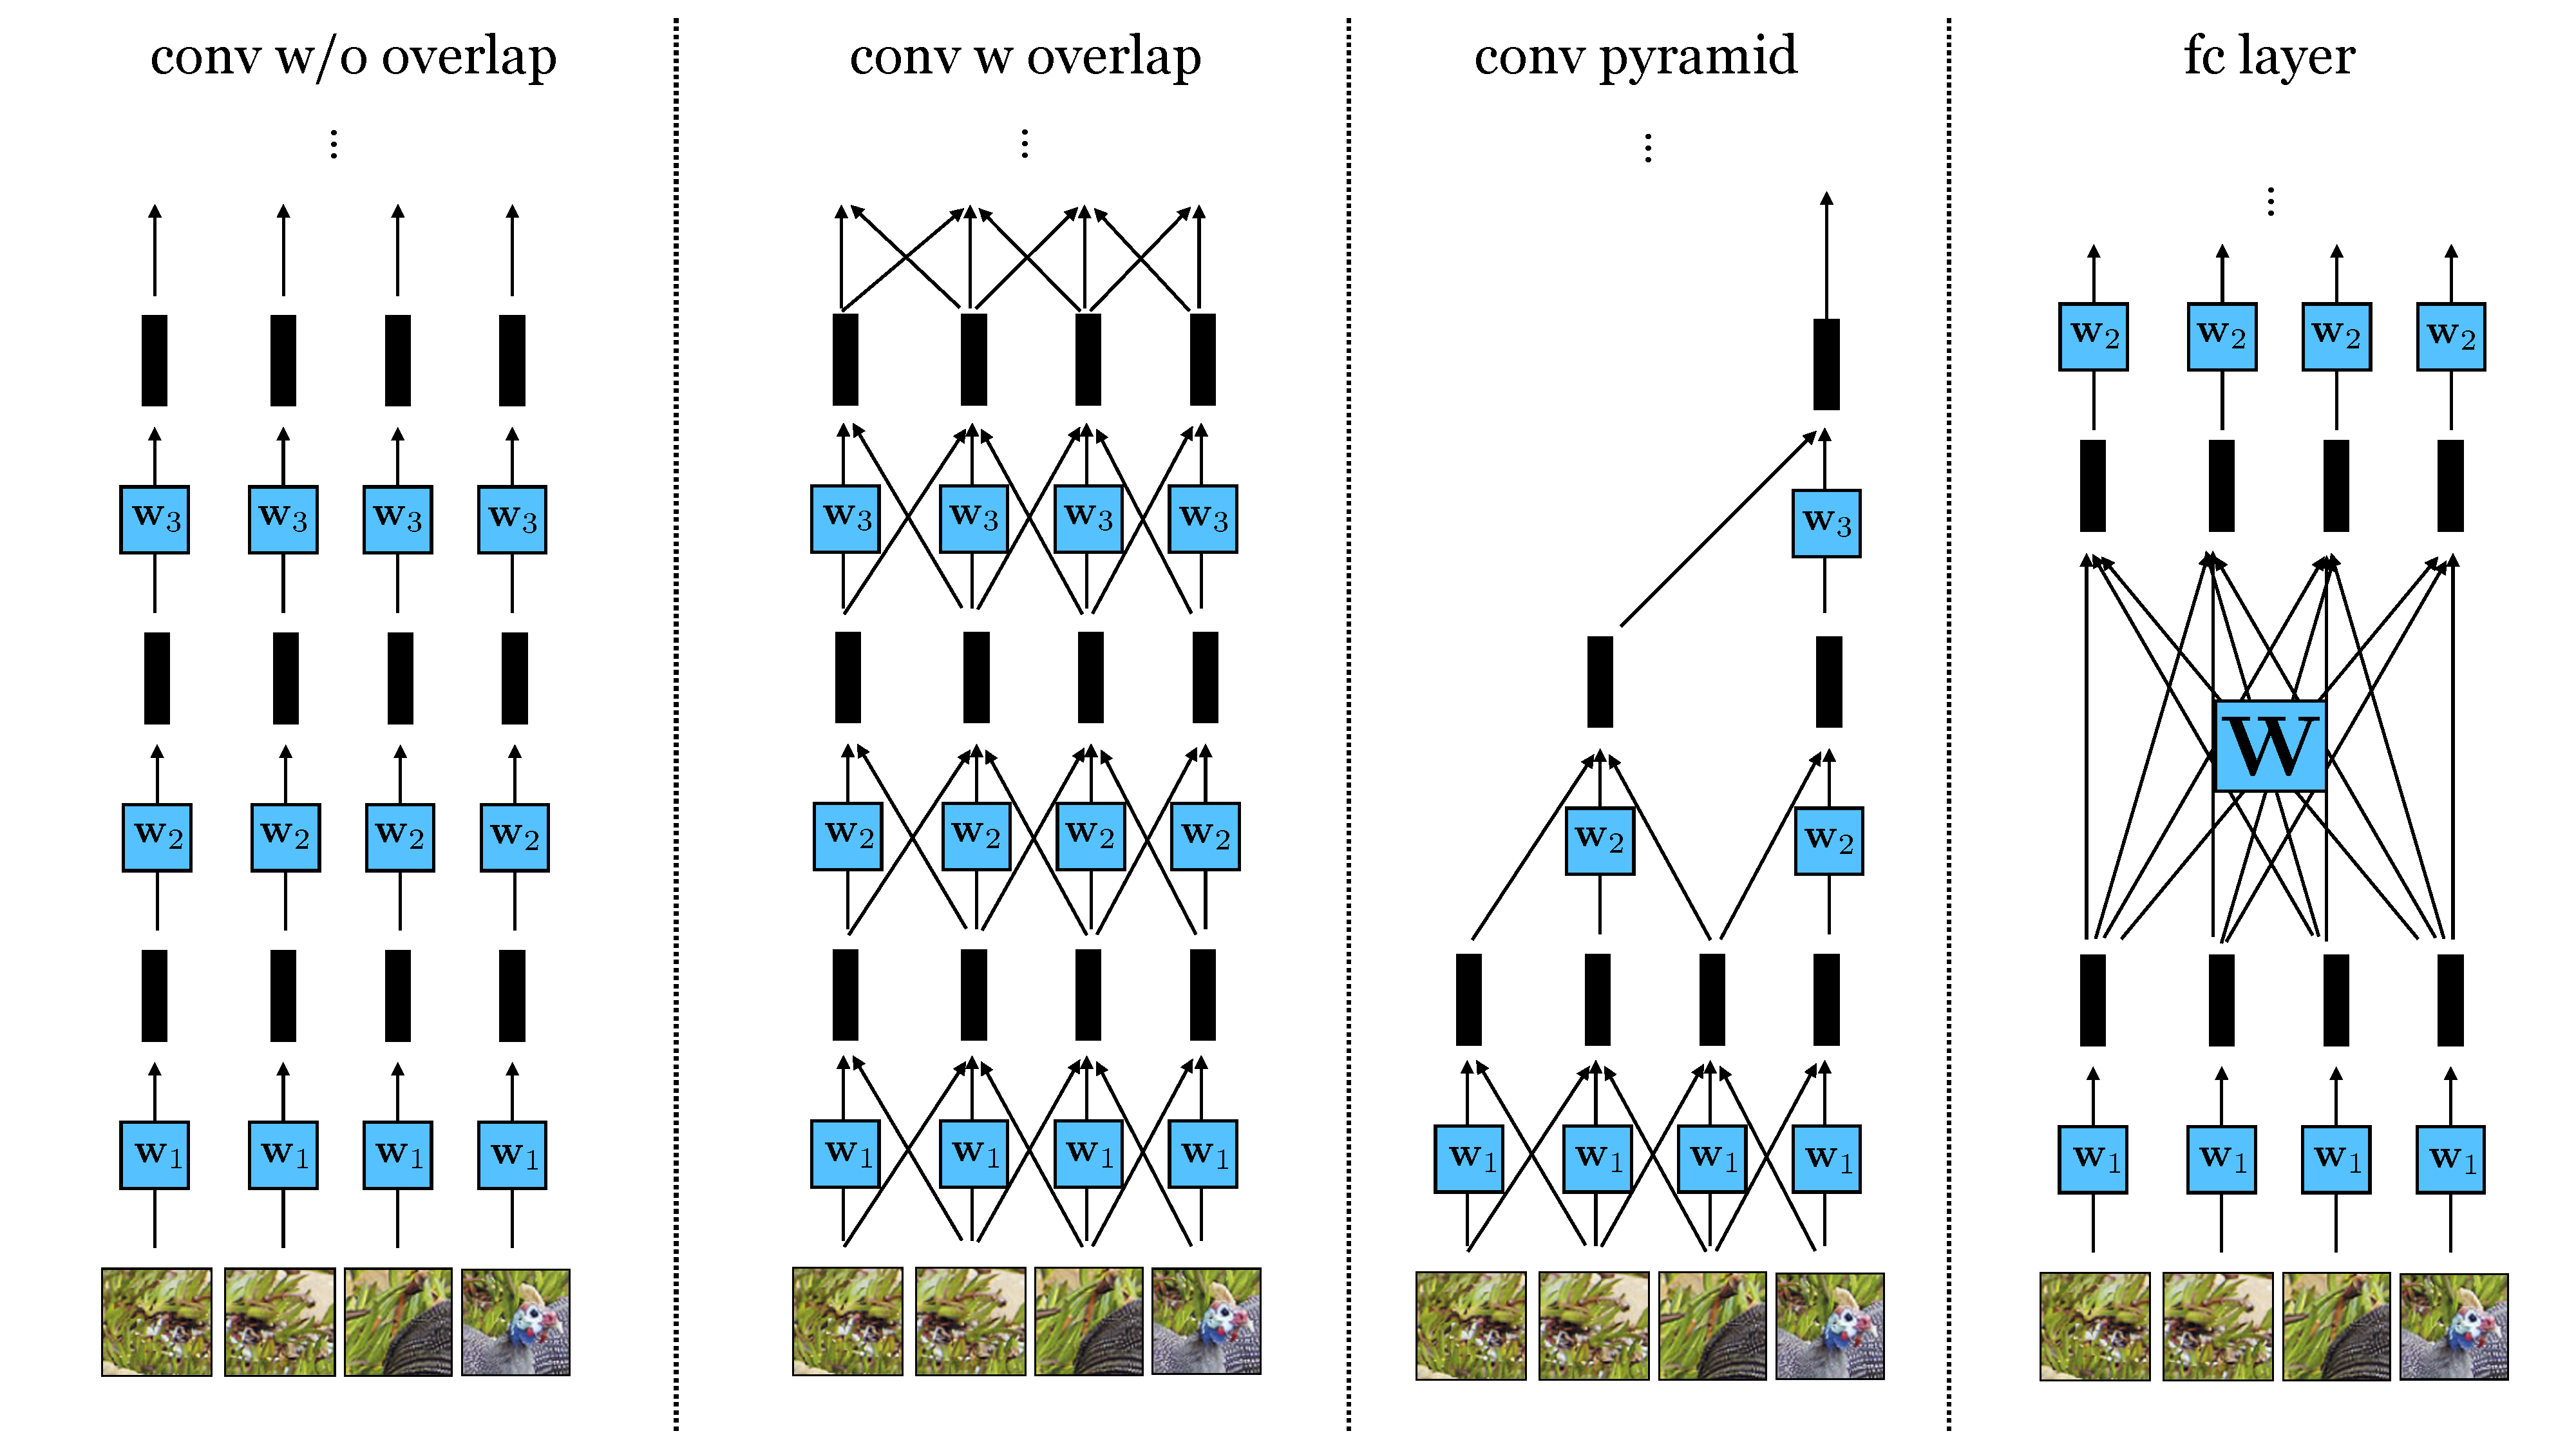
\includegraphics[width=1.0\linewidth]{./figures/transformers/token_mixing_strats.pdf}
% \end{figure}

\section{The Attention Layer}
\index{Attention!Attention layers}\textbf{Attention layers} define a special kind of linear combination of tokens. Rather than parameterizing the linear combination with a matrix of free parameters $\mathbf{W}$, attention layers use a different matrix, which we call the attention matrix $\mathbf{A}$. The important difference between $\mathbf{A}$ and $\mathbf{W}$ is that $\mathbf{A}$ is \textit{data-dependent}, that is, the values of $\mathbf{A}$ are a function the data input to the network. In addition, $\mathbf{A}$ typically only contains non-negative values, consistent with thinking of it as a matrix that allocates how much (non-negative) attention we pay to each input token. In the diagram below (\fig{\ref{fig:transformers:fc_vs_attn}}), we indicate the data-dependency with the function labeled $f$, and we color the attention matrix red to indicate that it is constructed from \textit{transformed data} rather than being free parameters (for which we use the color blue):\marginnote{Here, we describe attention as fc layers with data-dependent weights. We could have instead described attention as a kind of \index{Dynamic pooling}\textbf{dynamic pooling}, which is mean pooling but using a weighted average where the weights are dynamically decided based on the input data.}[-3.5cm]
\begin{figure}[h]
    \centerline{
        \begin{minipage}{.3\linewidth}
            \centering
            \begin{tikzpicture}
                %
                \def\Nnodes{3}
                \def\Nlayers{2}
                \def\layerheight{1.8}
                \def\neuronrad{0.35}
                \def\neuronstep{0.7}
                \foreach \x in {1,...,\Nnodes} {
                        \draw (\neuronstep*\x-\neuronrad/4,(\layerheight-\layerheight-\neuronrad) rectangle ++(\neuronrad/2,\neuronrad*2);
                    }
                \draw (\neuronstep*2-\neuronrad/4,(\layerheight*2-\layerheight-\neuronrad) rectangle ++(\neuronrad/2,\neuronrad*2);

                % mixing layer 1
                \foreach \xi in {1,...,\Nnodes} {
                        \draw [thick] [nn_edge] (\neuronstep*\xi,\neuronrad) -- (\neuronstep*2,\layerheight-\neuronrad);
                    }
                %
                \draw (0,0) node {$\tin$};
                \draw (0,1.8) node {$\mathbf{t}_\texttt{out}$};
                \draw (1.4,0.5*\layerheight) node[draw,rectangle,fill=white] {$\color{param_color_dark}\mathbf{W}$};
                %\draw (3.15,.5*\layerheight) node {$\Longrightarrow$};
                \draw (1.4,1.5*\layerheight) node {\texttt{fc} layer};
            \end{tikzpicture}
        \end{minipage}
        \begin{minipage}{.24\linewidth}
            \centering
            \begin{tikzpicture}
                %
                \def\Nnodes{3}
                \def\Nlayers{2}
                \def\layerheight{1.8}
                \def\neuronrad{0.3}
                \def\neuronstep{0.7}
                \foreach \x in {1,...,\Nnodes} {
                        \draw (\neuronstep*\x-\neuronrad/4,(\layerheight-\layerheight-\neuronrad) rectangle ++(\neuronrad/2,\neuronrad*2);
                    }
                \draw (\neuronstep*2-\neuronrad/4,(\layerheight*2-\layerheight-\neuronrad) rectangle ++(\neuronrad/2,\neuronrad*2);
                % mixing layer 1
                \foreach \xi in {1,...,\Nnodes} {
                        \draw [thick] [nn_edge] (\neuronstep*\xi,\neuronrad) -- (\neuronstep*2,\layerheight-\neuronrad);
                    }
                %
                \draw (1.4,0.5*\layerheight) node[draw,rectangle,fill=white] {$\color{data_color_dark}\mathbf{A}$};
                %\draw (2.4, 0.5*\layerheight) node {$\Bigg\}$};
                %\draw [thick] [nn_edge] (2.5,0)  .. controls (2.7,0.25*\layerheight) .. (2.0,0.5*\layerheight);
                \draw [thick,dotted] [nn_edge] (2.7,-\neuronrad) arc
                    [
                        start angle=0,
                        end angle=90.1,
                        x radius=0.8cm,
                        y radius=1.2cm
                    ];
                \draw (2.8,0.3*\layerheight) node {$f$};
                \draw (1.4,1.5*\layerheight) node {\texttt{attn} layer};
            \end{tikzpicture}
        \end{minipage}
    }
    \caption{Fully-connected layers versus attention layers.}
    \label{fig:transformers:fc_vs_attn}
\end{figure}

The equation for an attention layer is the same as for a linear layer except that the weights are a function of some other data (left unspecified for now but we will see concrete examples subsequently):
\begin{align}
    \mathbf{A} & = f(\ldots) \quad\quad \triangleleft \text{ attention} \\
    \tout      & = \mathbf{A}\tin
\end{align}

The key question, of course, is what exactly is $f$? What inputs does $f$ depend on and what is $f$'s mathematical form? Before writing out the exact equations, we will start with the intuition: $f$ is a function that determines how much attention to apply to each token in $\tin$; because this layer is just a weighted combination of tokens, $f$ is simply determining the weights in this combination. The $f$ can depend on any number of input signals that tell the net what to pay attention to.%$f$ is a function that makes it so each token gets to ``attend" over the input data to decide how to update its representation.

As a concrete example, consider that we want to be able to ask questions about different objects in our safari example image, such as how many animals are in the photo. Then one strategy would be to attend to each token that represents an animal's head, and then just count them up. The $f$ would take as input the text query, and would produce as output weights $\mathbf{A}$ that are high for the $\tin$ tokens that correspond to any animal's head and are low for all other $\tin$ tokens. If we train such a system to answer questions about counting animals, then the token code vectors might naturally end up encoding a feature that represents the number of animal heads in their receptive field; after all, this would be a solution that would solve our problem (it would minimize the loss and correctly answer the question). Other solutions might be possible, but we will focus on this intuitive solution, which we illustrate in \fig{\ref{fig:transformers:attention_layer_safari_query_cartoon}}.

%As a concrete example, consider that we want to be able to ask questions about different objects in an image, such as ``what color is the bird's head?" Then we can use attention to direct the model to focus on just the object in question -- the bird's head in this example. $f$ would take as input the text query, and would produce as output weights $\mathbf{A}$ that are high for the $\tin$ tokens that correspond to any bird head's and are low for all other $\tin$ tokens. If we train such as system to answer questions about color, then the token codes might end up representing the color of the object in their receptive field; after all, this would be a solution that would solve our problem (it would minimize the loss and correctly answer the question). Other solutions might be possible, but we will focus on this intuitive solution.

What's neat here is that attention gives us a way to make the layer dynamically change its behavior in response to different input questions; asking different questions results in different answers, as is visualized below in \fig{\ref{fig:transformers:attention_layer_safari_query_cartoon}}.
\begin{figure}[h!]
    \centerline{
        \begin{tikzpicture}
            \draw (0, 0) node[inner sep=0] {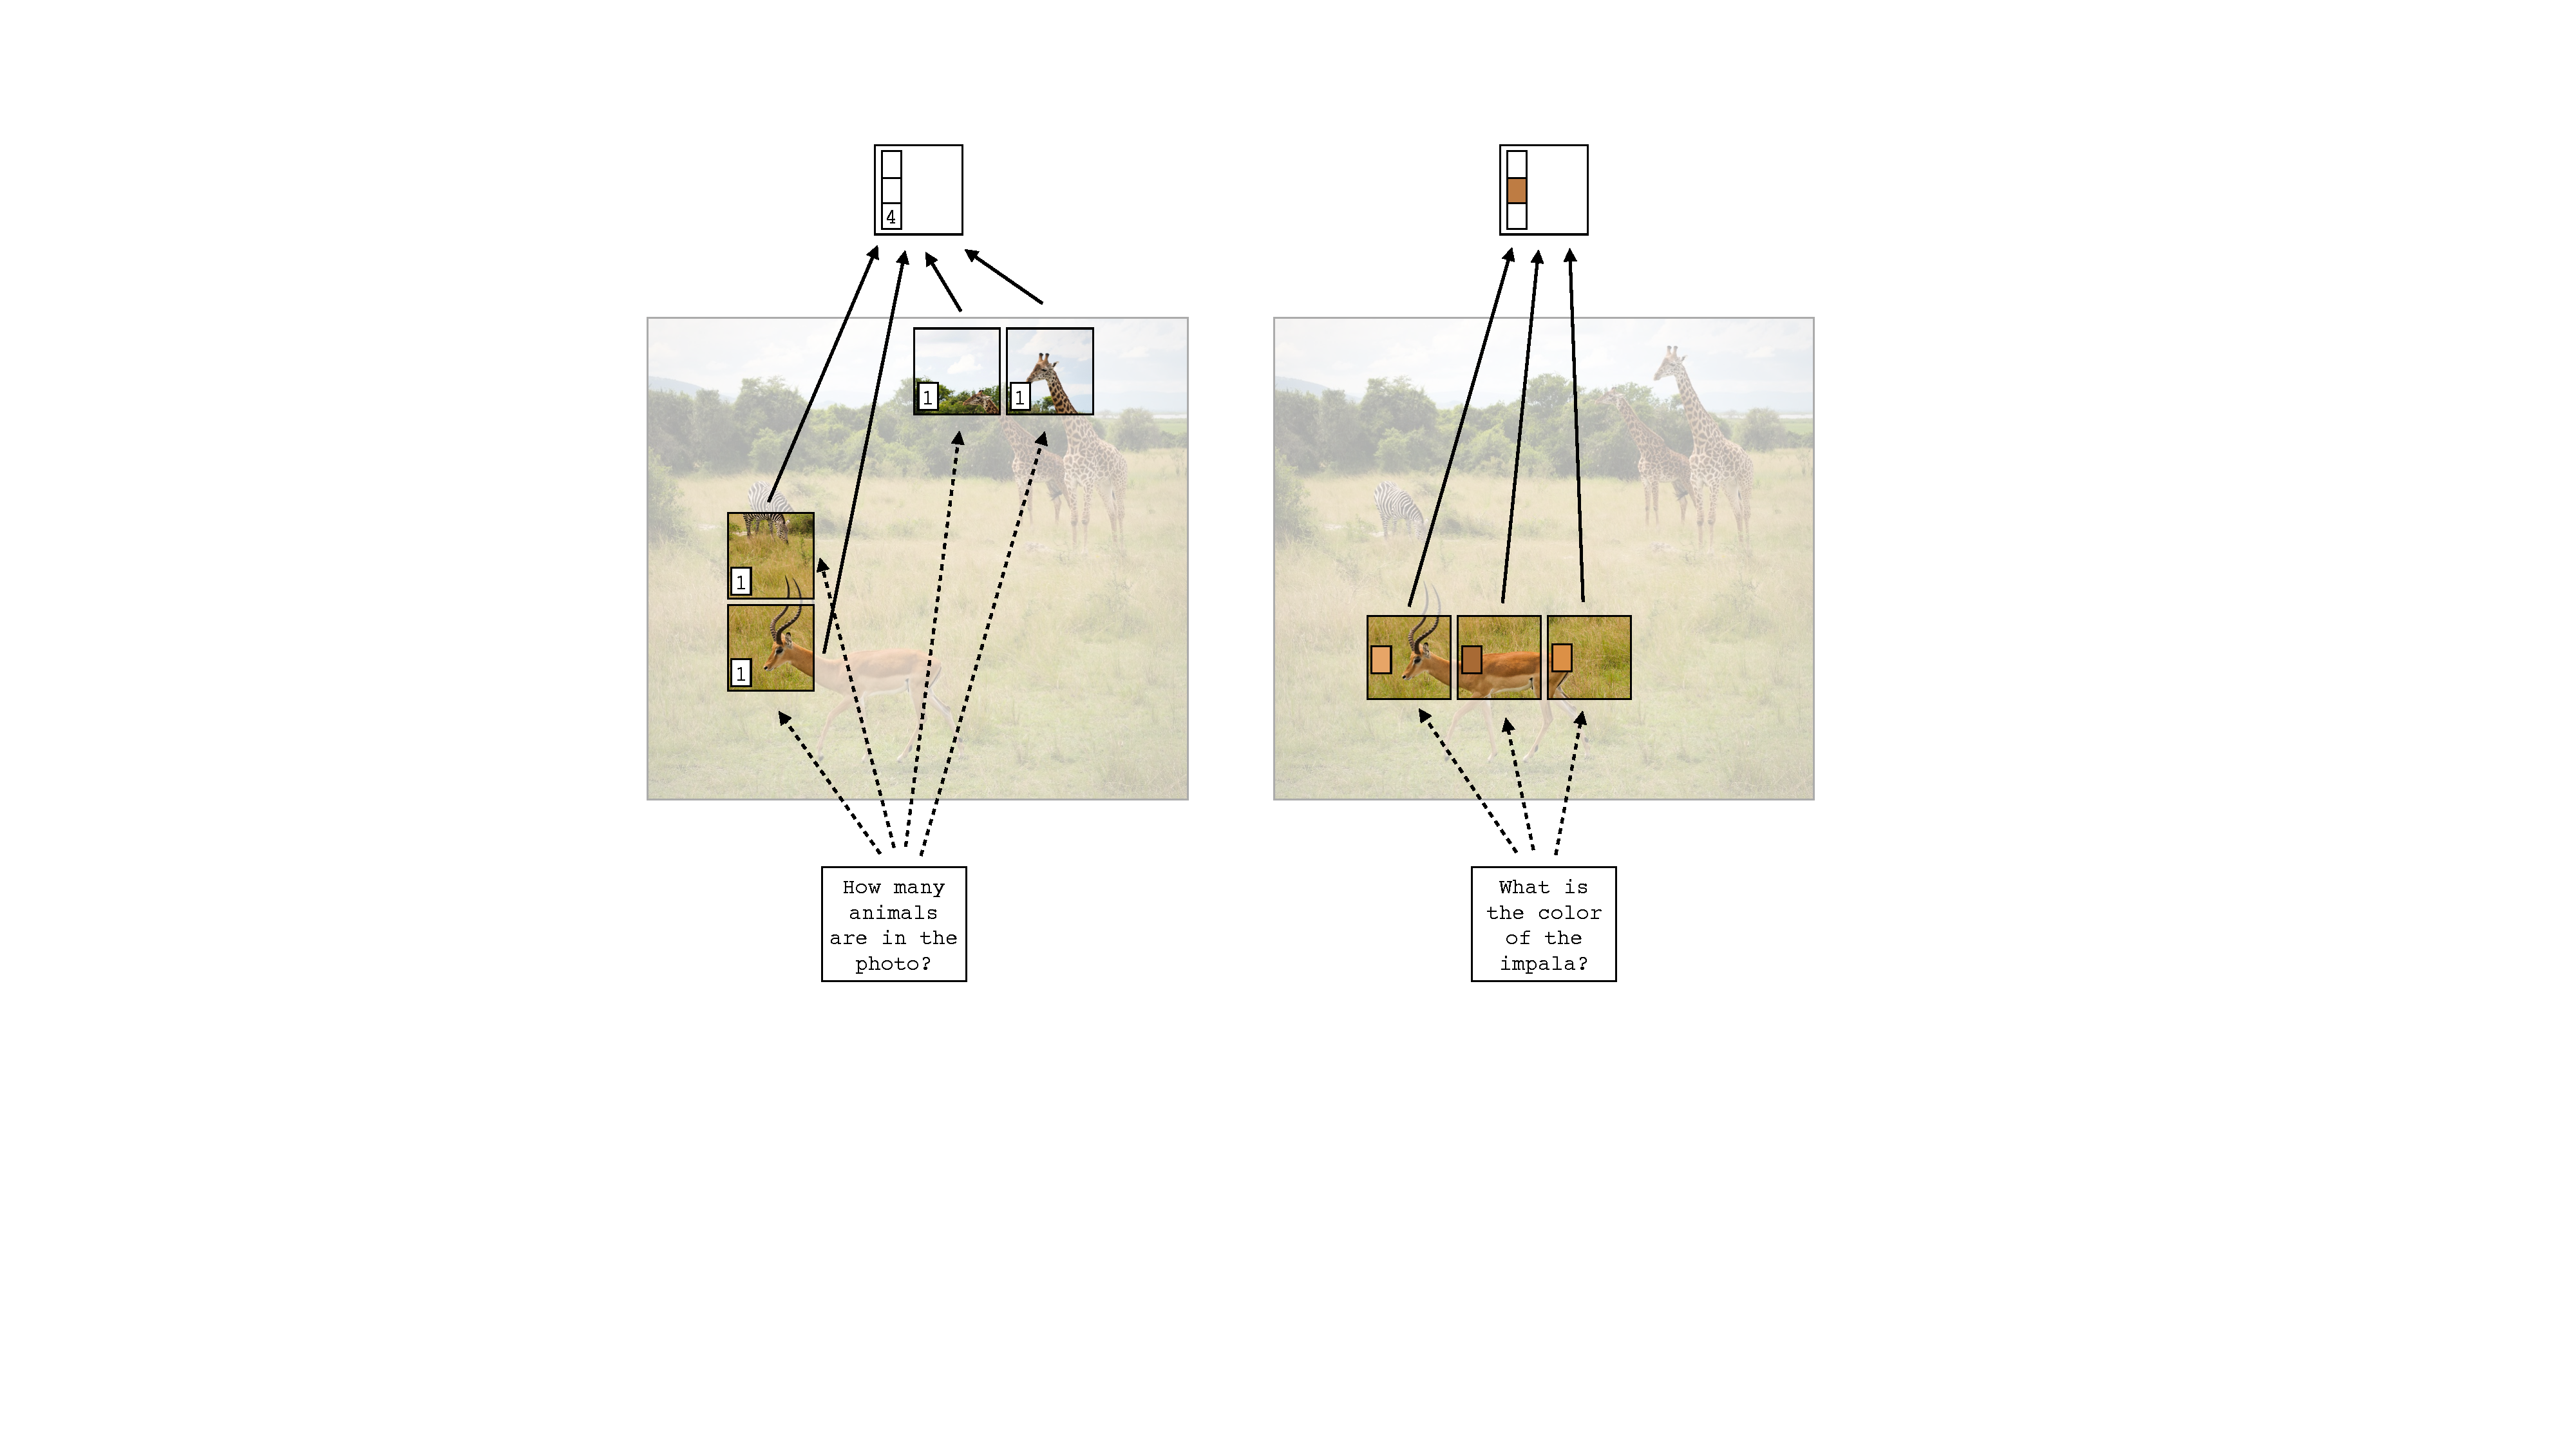
\includegraphics[width=0.75\linewidth]{./figures/transformers/attention_layer_safari_query_cartoon.pdf}};
            \draw (-6.7, 0) node {$\tin$}; \draw (-6.2,-2) -- (-6.2,2);
            \draw (-6.7, 3.5) node {$\mathbf{t}_\texttt{out}$}; \draw (-6.2,3.0) -- (-6.2,4.0);
            \draw (-1.5,-1.55) node {\texttt{attention}};
            \draw (-4.5, 2) node {\texttt{sum}};
        \end{tikzpicture}
    }
    \caption{How attention can be allocated across different regions (tokens) in an image. The token code vectors consist of multiple dimensions and each can encode a different attribute of the token. To the left we show a dimension that encodes number of animal heads. To the right we show a different dimension that encodes color (or this could be three dimensions, coding RGB). The output token is a weighted sum over all the tokens attended to.}%To the left this sum could use weights of $1$ for each attended token, and to the right it could use weights of $\frac{1}{3}$ to compute the average color of all impala patches.}
    \label{fig:transformers:attention_layer_safari_query_cartoon}
\end{figure}

Let's walk through the logic of \fig{\ref{fig:transformers:attention_layer_safari_query_cartoon}}. Here we are imagining a token representation that can answer two different kinds of questions, one about number and the other about color. The representation we have come up with (which learning could have arrived at) is to encode in one dimension of the token vector a constant of value $1$, which will be used for counting up the number of attended tokens. In another set of dimensions we have the average RGB color of the patch the token represents. Note that tokens only directly represent image patches at the input to the network, right after the tokenization step; at deeper layers of the network, the tokens may be more abstract in what they represent. Each text query elicits a different allocation of attention, and we will get to exactly how that process works later. For now just consider that the text query assigns a scalar weight to each token depending on how well that token's content matches the query's content. The output token, $\mathbf{t}_{\texttt{out}}$, is the sum of all the tokens weighted by the attention scalars. This scheme will arrive at a reasonable answer to the questions if the text query ``How many animals are in this photo'' gives attention weight $1$ to just the tokens representing animal heads and the text query ``What is the color of the impala'' gives weight $\frac{1}{3}$ just to the impala tokens. Then the output vector in the former case contains the correct answer $4$ in the dimension that represents number of attended tokens, and contains the RGB values for brownish in the dimensions that represent average patch color.


Keeping this intuitive picture in mind, we will now turn to the equations that define the attention allocation function $f$. We will focus on the particular version of $f$ that appears in transformers, which is called \textbf{query-key-value attention}.

\subsection{Query-Key-Value Attention}
\index{Attention!Query-Key-Value}
Transformers use a particular kind of attention based on the idea of queries, keys, and values.\marginnote{The idea of queries, keys, and values comes from databases, where a database cell holds a \textit{value}, which is retrieved when a \textit{query} matches the cell's \textit{key}. Tokens are like database cells and attention is like retrieving information from the database of tokens.}[-1.2cm] In query-key-value attention, each token is associated with a \textbf{query} vector, a \textbf{key} vector, and a \textbf{value} vector.

We define these vectors as linear transformations of the token's code vector, projecting to query/key/value vectors of length $m$. For a token $\mathbf{t}$, we have:
\begin{align}
    \mathbf{q} & = \mathbf{W}_q \mathbf{t} \quad\quad \triangleleft \text{ query} \\
    \mathbf{k} & = \mathbf{W}_k \mathbf{t} \quad\quad \triangleleft \text{ key}   \\
    \mathbf{v} & = \mathbf{W}_v \mathbf{t} \quad\quad \triangleleft \text{ value}
\end{align}
\marginnote{Here is a question to think about: Could you use other differentiable functions to compute the query, value, and key? Would that be useful?}[2.4cm]

%Just like the token's code vector, we can think of these vectors as additional members of the structure $t$. 





In transformers, all inputs to the net are tokenized, so the textual question ``How many animals are in the photo?'' will also be represented as a token.\marginnote{We do not cover them in this book, but methods from natural language processing can be used to transform text into a token, or into a sequence of tokens.}[1.8cm] This token will submit its query vector, $\mathbf{q}_{\texttt{question}}$ to be matched against the keys of the tokens that represent different patches in the image; the similarity between the query and the key determines the amount of attention weight the query will apply to the token with that key. The most common measure of similarity between a query $\mathbf{q}$ and a key $\mathbf{k}$ is the dot product $\mathbf{q}^\transpose\mathbf{k}$. Querying each token in $\tin$ in this way gives us a vector of similarities: %We can think of this operation in a few equivalent ways:
\begin{align}
    \mathbf{s} = [s_1, \ldots, s_N]^\transpose & = [\mathbf{q}_{\texttt{question}}^\transpose\mathbf{k}_1, \ldots, \mathbf{q}_{\texttt{question}}^\transpose\mathbf{k}_N]^\transpose \label{eqn:transformers:attention_question_keys}
\end{align}
%All these operations have the same meaning, but you may find it especially useful to recognize this operation as a convolution between a filter $\mathbf{q}_{\texttt{question}}$, with kernel size 1, and a multichannel 1D signal $\Kin$. The query vector is sliding over all the token keys and checking which ones match best, and the output is single channel 1D ``heatmap'' of which tokens matched. 

We then normalize the vector $\mathbf{s}$ using the softmax function to give us our attention weights $\mathbf{a} \in \mathbb{R}^{N \times 1}$, and finally, rather than applying $\mathbf{a}$ over token codes directly (i.e., taking a weighted sum over tokens), we take a weighted sum over token value vectors, to obtain $\tout$: %(note that here $\mathbf{A} \in \mathbb{R}^{1 \times N}$ because we only have one output token; later we will see a case where $\mathbf{A} \in \mathbb{R}^{N \times N}$):
\begin{align}
    %\mathbf{s} &= \mathbf{q}_{\texttt{question}} \circ \Kin\\ %[\mathbf{q}_{\texttt{question}}^T\mathbf{k}_1, \ldots, \mathbf{q}_{\texttt{question}}^T\mathbf{k}_N]\\
    \mathbf{a} & = \texttt{softmax}(\mathbf{s}) \\
    \tout      & = \begin{bmatrix}
                       a_1\mathbf{v}_1^\transpose \\
                       \vdots                     \\
                       a_N\mathbf{v}_N^\transpose \\
                   \end{bmatrix}
\end{align}
\marginnote{$\mathbf{v}_1$ is the value vector for $\mathbf{t}_1 = \tinOne$, and so forth.}[-1.4cm]
Figure \ref{fig:transformers:attn_arch1} visualizes these steps.
\marginnote{We use the following color scheme here and later in this chapter:
    \medbreak
    \centerline{
        \begin{tikzpicture}
            \def\neuronrad{0.25}
            \draw [fill=query_color] (0,0) rectangle ++(\neuronrad/2,\neuronrad*2);
            \draw [fill=key_color] (1,0) rectangle ++(\neuronrad/2,\neuronrad*2);
            \draw [fill=value_color] (2,0) rectangle ++(\neuronrad/2,\neuronrad*2);
            %
            \draw (0,0.8) node {query};
            \draw (1,0.8) node {key};
            \draw (2,0.8) node {value};
        \end{tikzpicture}
    }}[-4cm]

\begin{figure}[h!]
    \centerline{
        \begin{tikzpicture}
            \draw (0, 0) node[inner sep=0] {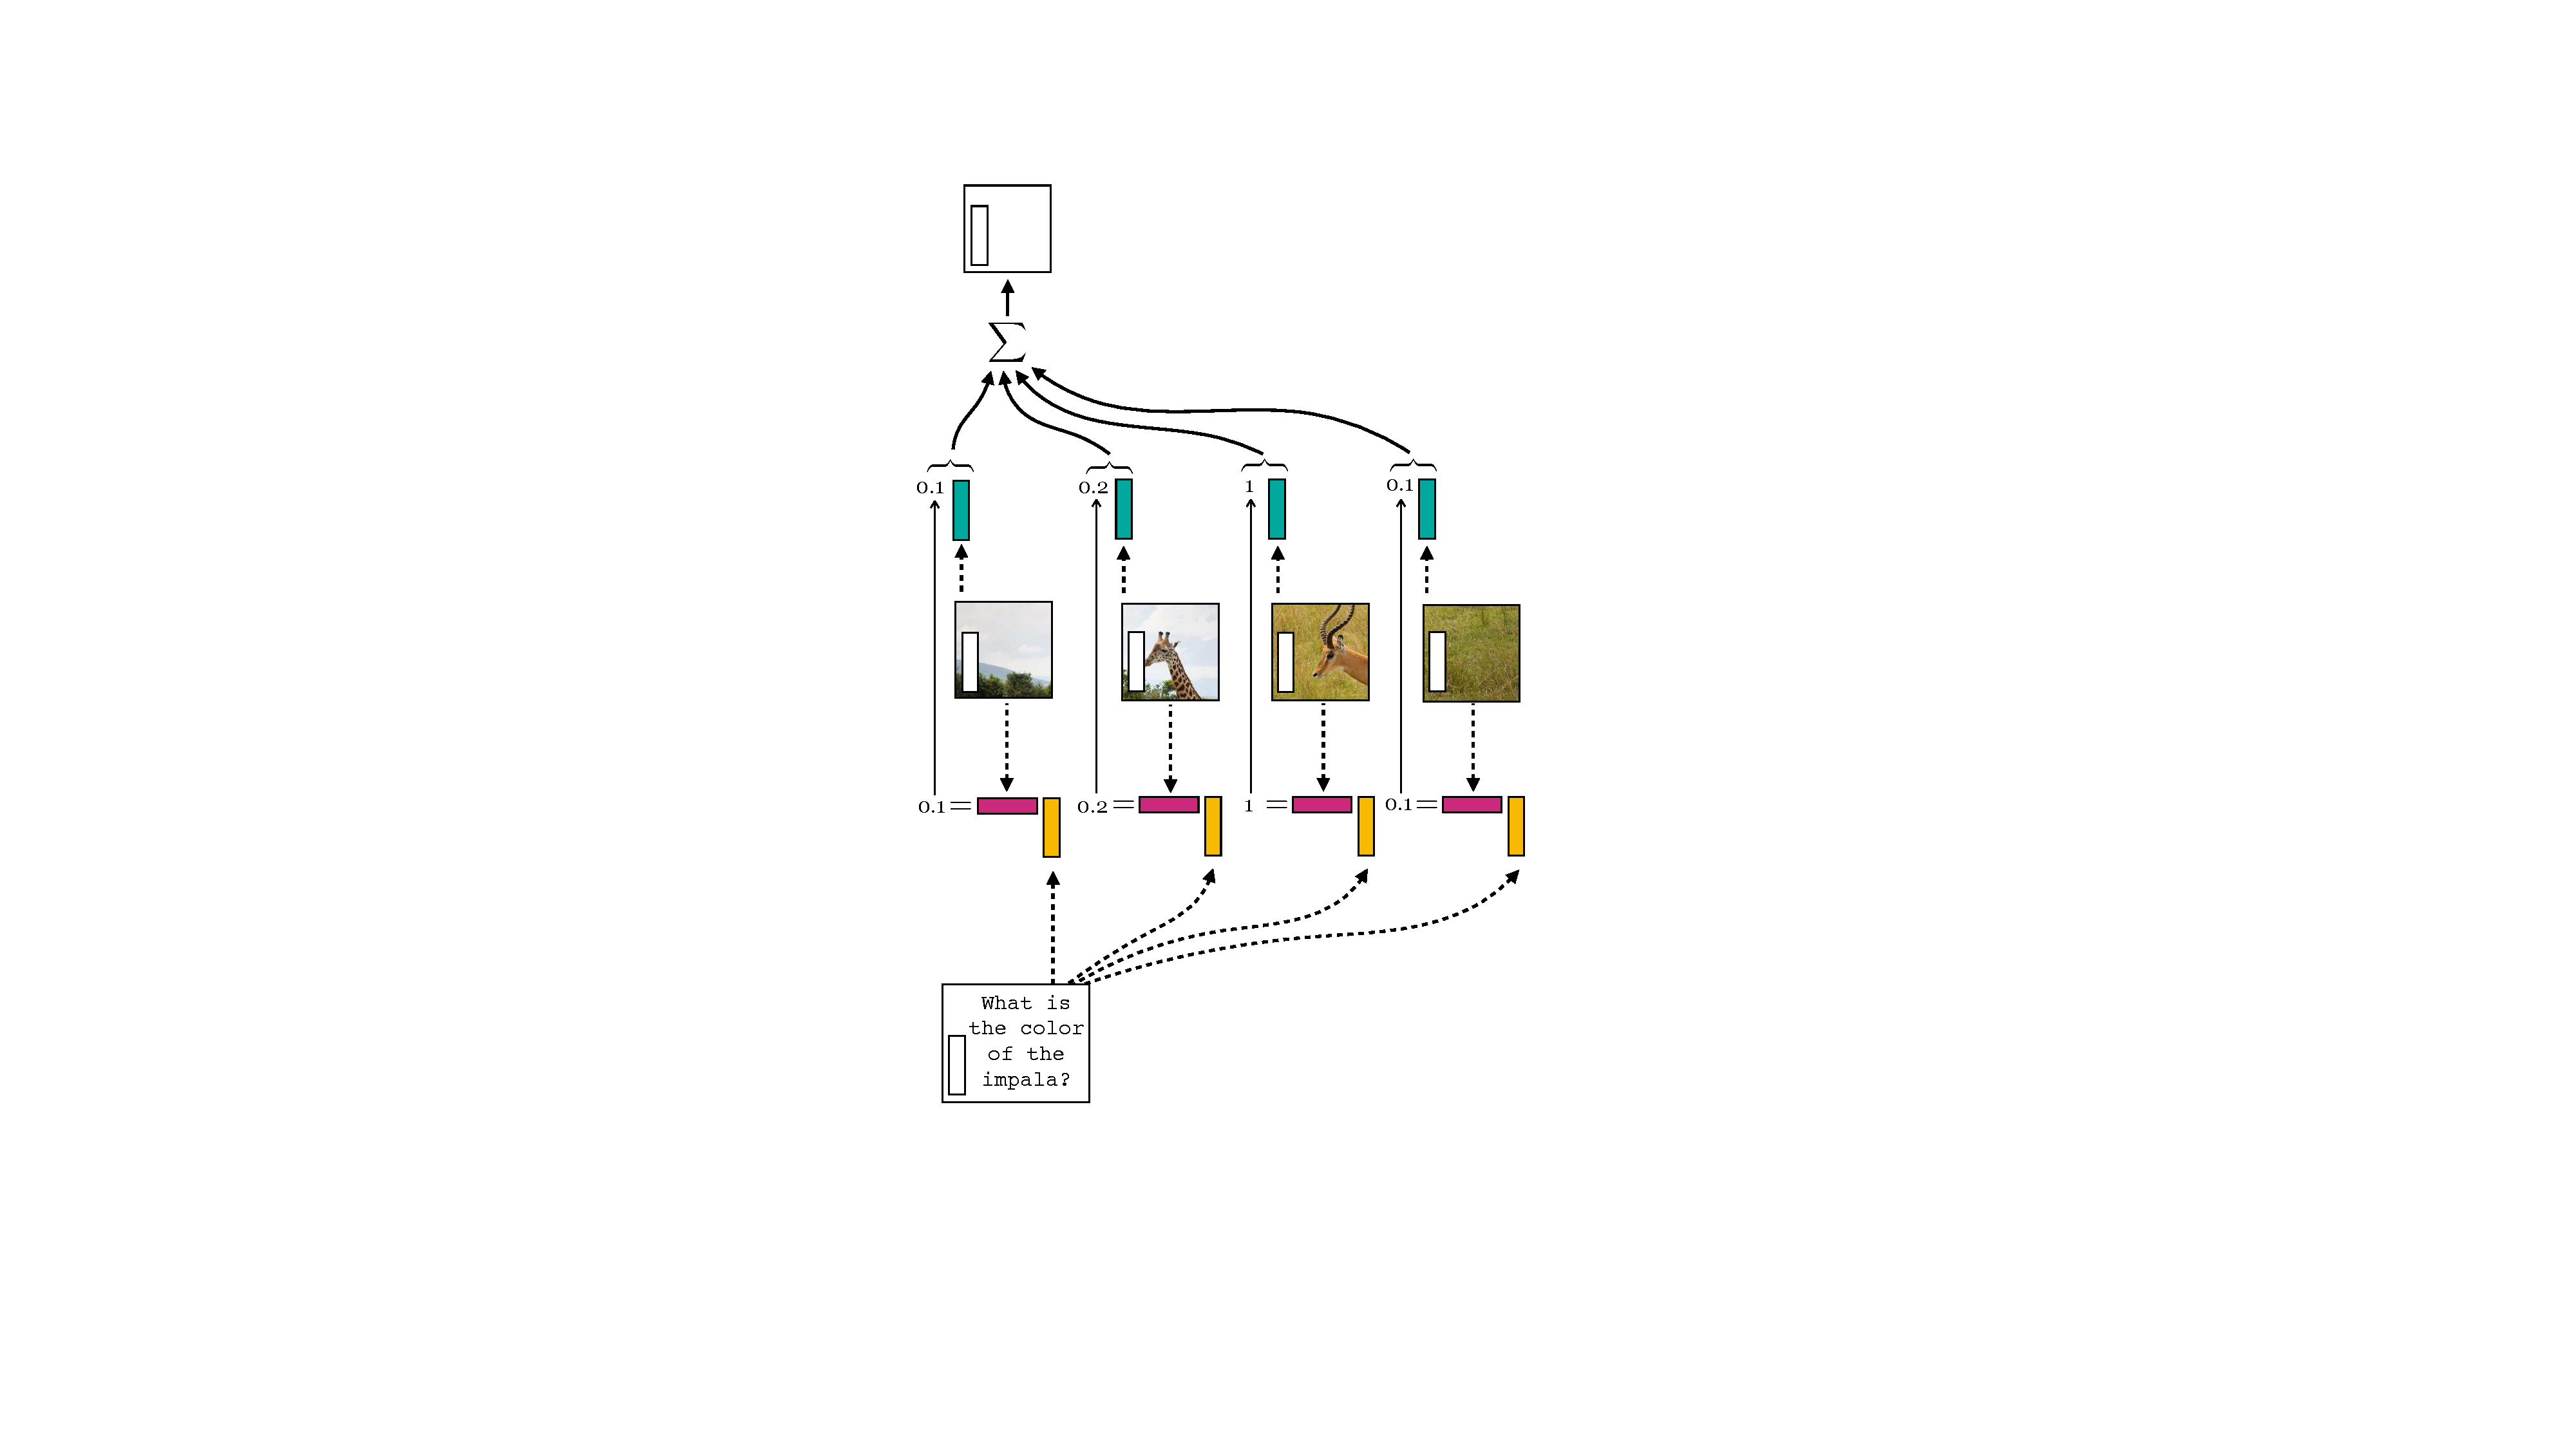
\includegraphics[width=0.39\linewidth]{./figures/transformers/attn_arch1_safari.pdf}};
            \draw (-3.75, 0) node {$\tin$}; \draw (-3.25,-0.5) -- (-3.25,0.5);
            \draw (-3.75, 3.75) node {$\mathbf{t}_\texttt{out}$}; \draw (-3.25,3.25) -- (-3.25,4.25);
            \draw (4, 0.65) node {$\} \quad \texttt{value()}$};
            \draw (4, -1) node {$\Big\} \quad \texttt{key()  }$};
            \draw (4, -2.5) node {$\Big\} \quad \texttt{query()}$};
        \end{tikzpicture}
    }
    \caption{Mechanics of an attention layer. Queries from the question match keys from the tokens representing the impala; value vectors of the impala tokens then contribute the most to the sum that yields $\mathbf{t}_{\texttt{out}}$'s code vector. (Softmax omitted in this example.)}
    \label{fig:transformers:attn_arch1}
\end{figure}

\subsection{Self-Attention}
As we have now seen, attention is a general-purpose way of dynamically pooling information in one set of tokens based on queries from a different set of tokens. The next question we will consider is which tokens should be doing the querying and which should we be matching against? In the example from the last section, the answer was intuitive because we had a textual question that was asking about content in a visual image, so naturally the text gives the query and we match against tokens that represent the image. But can we come up with a more generic architecture where we don't have to hand design which tokens interact in which ways?

\index{Attention!Self-attention}\textbf{Self-attention} is just such an architecture. The idea is that on a self-attention layer, \textit{all} tokens submit queries, and for each of these queries, we take a weighted sum over \textit{all} tokens in that layer. If $\tin$ is a set of $N$ input tokens, then we have $N$ queries, $N$ weighted sums, and $N$ output tokens to form $\tout$. This is visualized below in \fig{\ref{fig:transformers:self_attn_layer}}.
\begin{figure}[h]
    \centerline{
        \begin{tikzpicture}
            %
            \def\Nnodes{3}
            \def\Nlayers{2}
            \def\layerheight{1.8}
            \def\neuronrad{0.3}
            \def\neuronstep{0.7}
            \foreach \x in {1,...,\Nnodes} {
                    \foreach \y in {1,...,\Nlayers} {
                            \draw (\neuronstep*\x-\neuronrad/4,(\layerheight*\y-\layerheight-\neuronrad) rectangle ++(\neuronrad/2,\neuronrad*2);
                        }
                }
            % mixing layer 1
            \foreach \xi in {1,...,\Nnodes} {
                    \foreach \xj in {1,...,\Nnodes} {
                            \draw [thick] [nn_edge] (\neuronstep*\xi,\neuronrad) -- (\neuronstep*\xj,\layerheight-\neuronrad);
                        }
                }
            %
            \draw (1.4,0.5*\layerheight) node[draw,rectangle,fill=white] {$\color{data_color_dark}\mathbf{A}$};
            \draw (2.4, 0) node {$\Big\}$};
            %\draw (2.4, 0.5*\layerheight) node {$\Bigg\}$};
            %\draw [thick] [nn_edge] (2.5,0)  .. controls (2.7,0.25*\layerheight) .. (2.0,0.5*\layerheight);
            \draw [thick] [nn_edge] (2.5,0) arc
                [
                    start angle=-70,
                    end angle=90,
                    x radius=0.4cm,
                    y radius =0.45cm
                ] ;
            \draw (3.0,0.25*\layerheight) node {$f$};
            \draw (1.4,1.5*\layerheight) node {\texttt{self attn} layer};
            \draw (0,0) node {$\tin$};
            \draw (0,1.8) node {$\tout$};
        \end{tikzpicture}
    }
    \caption{A self-attention layer.}
    \label{fig:transformers:self_attn_layer}
\end{figure}
\vspace{-0.5cm}

%In the figure below we name the attention weight matrix as $\mathbf{A}$ (for ``affinity matrix", or, if you like ``attention matrix") and color it red since it is \textit{not} free learnable parameters but rather derived from \textit{activations} output by other parts of the network (which we will describe below):


To compute the query, key, and value for a set of input tokens, $\tin$, we apply the same linear transformations to each token in the set, resulting in matrices $\mathbf{Q}_{\texttt{in}}, \mathbf{K}_{\texttt{in}} \in \mathbb{R}^{N \times m}$ and $\mathbf{V}_{\texttt{in}} \in \mathbb{R}^{N \times d}$, where each row is the query/key/value for each token:
\marginnote{Note that the query and key vectors must have the same dimensionality, $m$, because we take a dot product between them. Conversely, the value vectors must match the dimensionality of the token code vectors, $d$, because these are summed up to produce the new token code vectors.}[-0.4cm]
\begin{align}
    \Qin                          & =
    \begin{bmatrix}
        \mathbf{q}_1^\transpose \\
        \vdots                  \\
        \mathbf{q}_N^\transpose \\
    \end{bmatrix}
    =
    \begin{bmatrix}
        (\mathbf{W}_q \mathbf{t}_1)^\transpose \\
        \vdots                                 \\
        (\mathbf{W}_q \mathbf{t}_N)^\transpose \\
    \end{bmatrix}
    = \tin\mathbf{W}_q^\transpose & \triangleleft \quad\quad \text{query matrix} \label{eqn:transformers:query_matrix} \\
    %
    \Kin                          & =
    \begin{bmatrix}
        \mathbf{k}_1^\transpose \\
        \vdots                  \\
        \mathbf{k}_N^\transpose \\
    \end{bmatrix}
    =
    \begin{bmatrix}
        (\mathbf{W}_k \mathbf{t}_1)^\transpose \\
        \vdots                                 \\
        (\mathbf{W}_k \mathbf{t}_N)^\transpose \\
    \end{bmatrix}
    = \tin\mathbf{W}_k^\transpose & \triangleleft \quad\quad \text{key matrix}                                         \\
    %
    \Vin                          & =
    \begin{bmatrix}
        \mathbf{v}_1^\transpose \\
        \vdots                  \\
        \mathbf{v}_N^\transpose \\
    \end{bmatrix}
    =
    \begin{bmatrix}
        (\mathbf{W}_v \mathbf{t}_1)^\transpose \\
        \vdots                                 \\
        (\mathbf{W}_v \mathbf{t}_N)^\transpose \\
    \end{bmatrix}
    = \tin\mathbf{W}_v^\transpose & \triangleleft \quad\quad \text{value matrix}
\end{align}

Finally, we have the attention equation:
\begin{align}
    \mathbf{A} & = f(\tin) = \texttt{softmax}\Big(\frac{\mathbf{Q}_{\texttt{in}}\mathbf{K}_{\texttt{in}}^\transpose}{\sqrt{m}}\Big) & \triangleleft \quad\quad \text{attention matrix} \\
    \tout      & = \mathbf{A}\mathbf{V}_{\texttt{in}}
\end{align}
% \begin{align}
%     \Qin &= \mathbf{w}_{q} \star \tin &\triangleleft \quad\quad \text{queries}\\
%     \Kin &= \mathbf{w}_{k} \star \tin &\triangleleft \quad\quad \text{keys}\\
%     \Vin &= \mathbf{w}_{v} \star \tin &\triangleleft \quad\quad \text{values}\\
%     \mathbf{A} &= f(\tin) = \texttt{softmax}\Big(\frac{\Qin\Kin^T}{\sqrt{d}}\Big) &\triangleleft \quad\quad \text{attention matrix}\\
%     \tout &= \mathbf{A}\Vin
% \end{align}
where the softmax is taken within each row (i.e., over the vector of matches for each separate query vector, like in \eqn{\ref{eqn:transformers:attention_question_keys}}). In expanded detail, here are the full mechanics of a self-attention layer (\fig{\ref{fig:transformers:attn_arch}}):
\begin{figure}[h]
    \centerline{
        \begin{tikzpicture}
            %
            \def\Nnodes{3}
            \def\Nlayers{2}
            \def\layerheight{1.1}
            \def\neuronrad{0.3}
            \def\neuronstep{0.9}
            % input layer
            \foreach \x in {1,...,\Nnodes} {
                    \def\y{1}
                    \draw (\neuronstep*\x-\neuronrad/4,(\layerheight*\y-\layerheight-\neuronrad) rectangle ++(\neuronrad/2,\neuronrad*2);
                }
            % pointwise nonlinearity
            \foreach \x in {1,...,\Nnodes} {
                    \draw [thick] [nn_edge] (\neuronstep*\x,\neuronrad) -- (\neuronstep*\x,\layerheight-\neuronrad);
                    \draw [thick] [nn_edge] (\neuronstep*\x,\neuronrad) -- (\neuronstep*\x-\neuronrad*0.5,\layerheight-\neuronrad);
                    \draw [thick] [nn_edge] (\neuronstep*\x,\neuronrad) -- (\neuronstep*\x-\neuronrad,\layerheight-\neuronrad);
                }
            % query-key-value layer
            \def\y{2}
            \foreach \x in {1,...,\Nnodes} {
            \draw [fill=value_color] (\neuronstep*\x-\neuronrad/4,(\layerheight*\y-\layerheight-\neuronrad) rectangle ++(\neuronrad/2,\neuronrad*2);
            \draw [fill=key_color] (\neuronstep*\x-\neuronrad/4-\neuronrad*0.5,(\layerheight*\y-\layerheight-\neuronrad) rectangle ++(\neuronrad/2,\neuronrad*2);
            \draw [fill=query_color] (\neuronstep*\x-\neuronrad/4-\neuronrad,(\layerheight*\y-\layerheight-\neuronrad) rectangle ++(\neuronrad/2,\neuronrad*2);
            }
            \draw [fill=key_color, very thick, draw=black, dashed] (\neuronstep-\neuronrad/4-\neuronrad*0.5,(\layerheight*\y-\layerheight-\neuronrad) rectangle ++(\neuronrad/2,\neuronrad*2);
            \draw [fill=query_color, very thick, draw=black, dashed] (\neuronstep-\neuronrad/4-\neuronrad,(\layerheight*\y-\layerheight-\neuronrad) rectangle ++(\neuronrad/2,\neuronrad*2);

            \foreach \x in {1,...,\Nnodes} {
                    \def\y{4}
                    \draw (\neuronstep*\x-\neuronrad/4,(\layerheight*\y-\layerheight-\neuronrad) rectangle ++(\neuronrad/2,\neuronrad*2);
                }
            % attn
            \def\y{1}
            \foreach \xi in {1,...,\Nnodes} {
                    \foreach \xj in {1,...,\Nnodes} {
                            \draw [thick] [nn_edge] (\neuronstep*\xi,\layerheight*\y+\neuronrad) -- (\neuronstep*\xj,\layerheight*2+\layerheight*\y-\neuronrad);
                        }
                }
            %
            \draw (1.8,2*\layerheight) node[draw,rectangle,fill=white] {$\color{data_color_dark}\mathbf{A}$};

            \def\offset{0.6}
            \draw (4, \offset+\layerheight) rectangle ++(1,1);
            \draw (4+0.5, \offset+\layerheight+0.5) node {$\color{data_color_dark}\mathbf{A}$};
            \draw [fill=gray, draw=black, dashed, dash pattern=on 1.75pt off 1.75pt, thick] (4+0.1, \offset+\layerheight+1-0.25) rectangle ++(\neuronrad/2,\neuronrad/2);
            \draw [fill=gray, draw=black, dashed, dash pattern=on 1.75pt off 1.75pt, thick] (\neuronstep-\neuronrad/4, 2*\layerheight-\neuronrad/4) rectangle ++(\neuronrad/2,\neuronrad/2);
            \draw (4+0.5, \offset+\layerheight+1+0.2) node[scale=0.7] {$N$};
            \draw (4-0.2, \offset+\layerheight+0.5) node[scale=0.7] {$N$};
            \draw (4+1+0.4, \offset+\layerheight+0.5) node {$=$};
            \foreach \x in {1,...,\Nnodes} {
                    \draw [fill=query_color] (6,\offset+\layerheight+\x*0.3+0.06-0.2) rectangle ++(\neuronrad*2,\neuronrad/2);

                    \draw [fill=key_color] (6.7+\x*0.3-0.2,\offset+\layerheight+0.32) rectangle ++(\neuronrad/2,\neuronrad*2);
                }

            \draw [fill=query_color, draw=black, very thick, dashed] (6,\offset+\layerheight+0.3*3+0.06-0.2) rectangle ++(\neuronrad*2,\neuronrad/2);
            \draw [fill=key_color, draw=black, very thick, dashed] (6.7+0.3-0.2,\offset+\layerheight+0.32) rectangle ++(\neuronrad/2,\neuronrad*2);

            \draw (5.8, \offset+\layerheight+2*0.2+0.1) node[scale=0.7] {$N$};
            \draw (6.3, \offset+\layerheight+4*0.2+0.3) node[scale=0.7] {$M$};
            \draw (7.2, \offset+\layerheight+4*0.2+0.3) node[scale=0.7] {$N$};
            \draw (7.8, \offset+\layerheight+2*0.2+0.25) node[scale=0.7] {$M$};
            \draw [thick] [nn_edge] (3,\layerheight) arc
                [
                    start angle=-140,
                    end angle=30,
                    x radius=3.0cm,
                    y radius =1.0cm
                ] ;
            \draw [thick] [nn_edge] (3.6,\layerheight+\offset+0.5) -- (2.9,\layerheight+\offset+0.5);

            \draw (3.8,3.8*\layerheight) node {\texttt{self attn} layer (expanded)};
            \draw (0,0) node {$\tin$};
            \draw (0,\layerheight*3) node {$\tout$};
            \draw (-0.9,\layerheight) node {$\Qin, \Kin, \Vin$};
        \end{tikzpicture}
    }
    \caption{Self-attention layer expanded. The nodes with the dashed outline correspond to each other; they represent one query being matched against one key to result in a scalar similarity value, in the gray box, which acts as a weight in the weighted sum computed by $\mathbf{A}$.}
    \label{fig:transformers:attn_arch}
\end{figure}
% \begin{figure}[h]
%     \centering
%     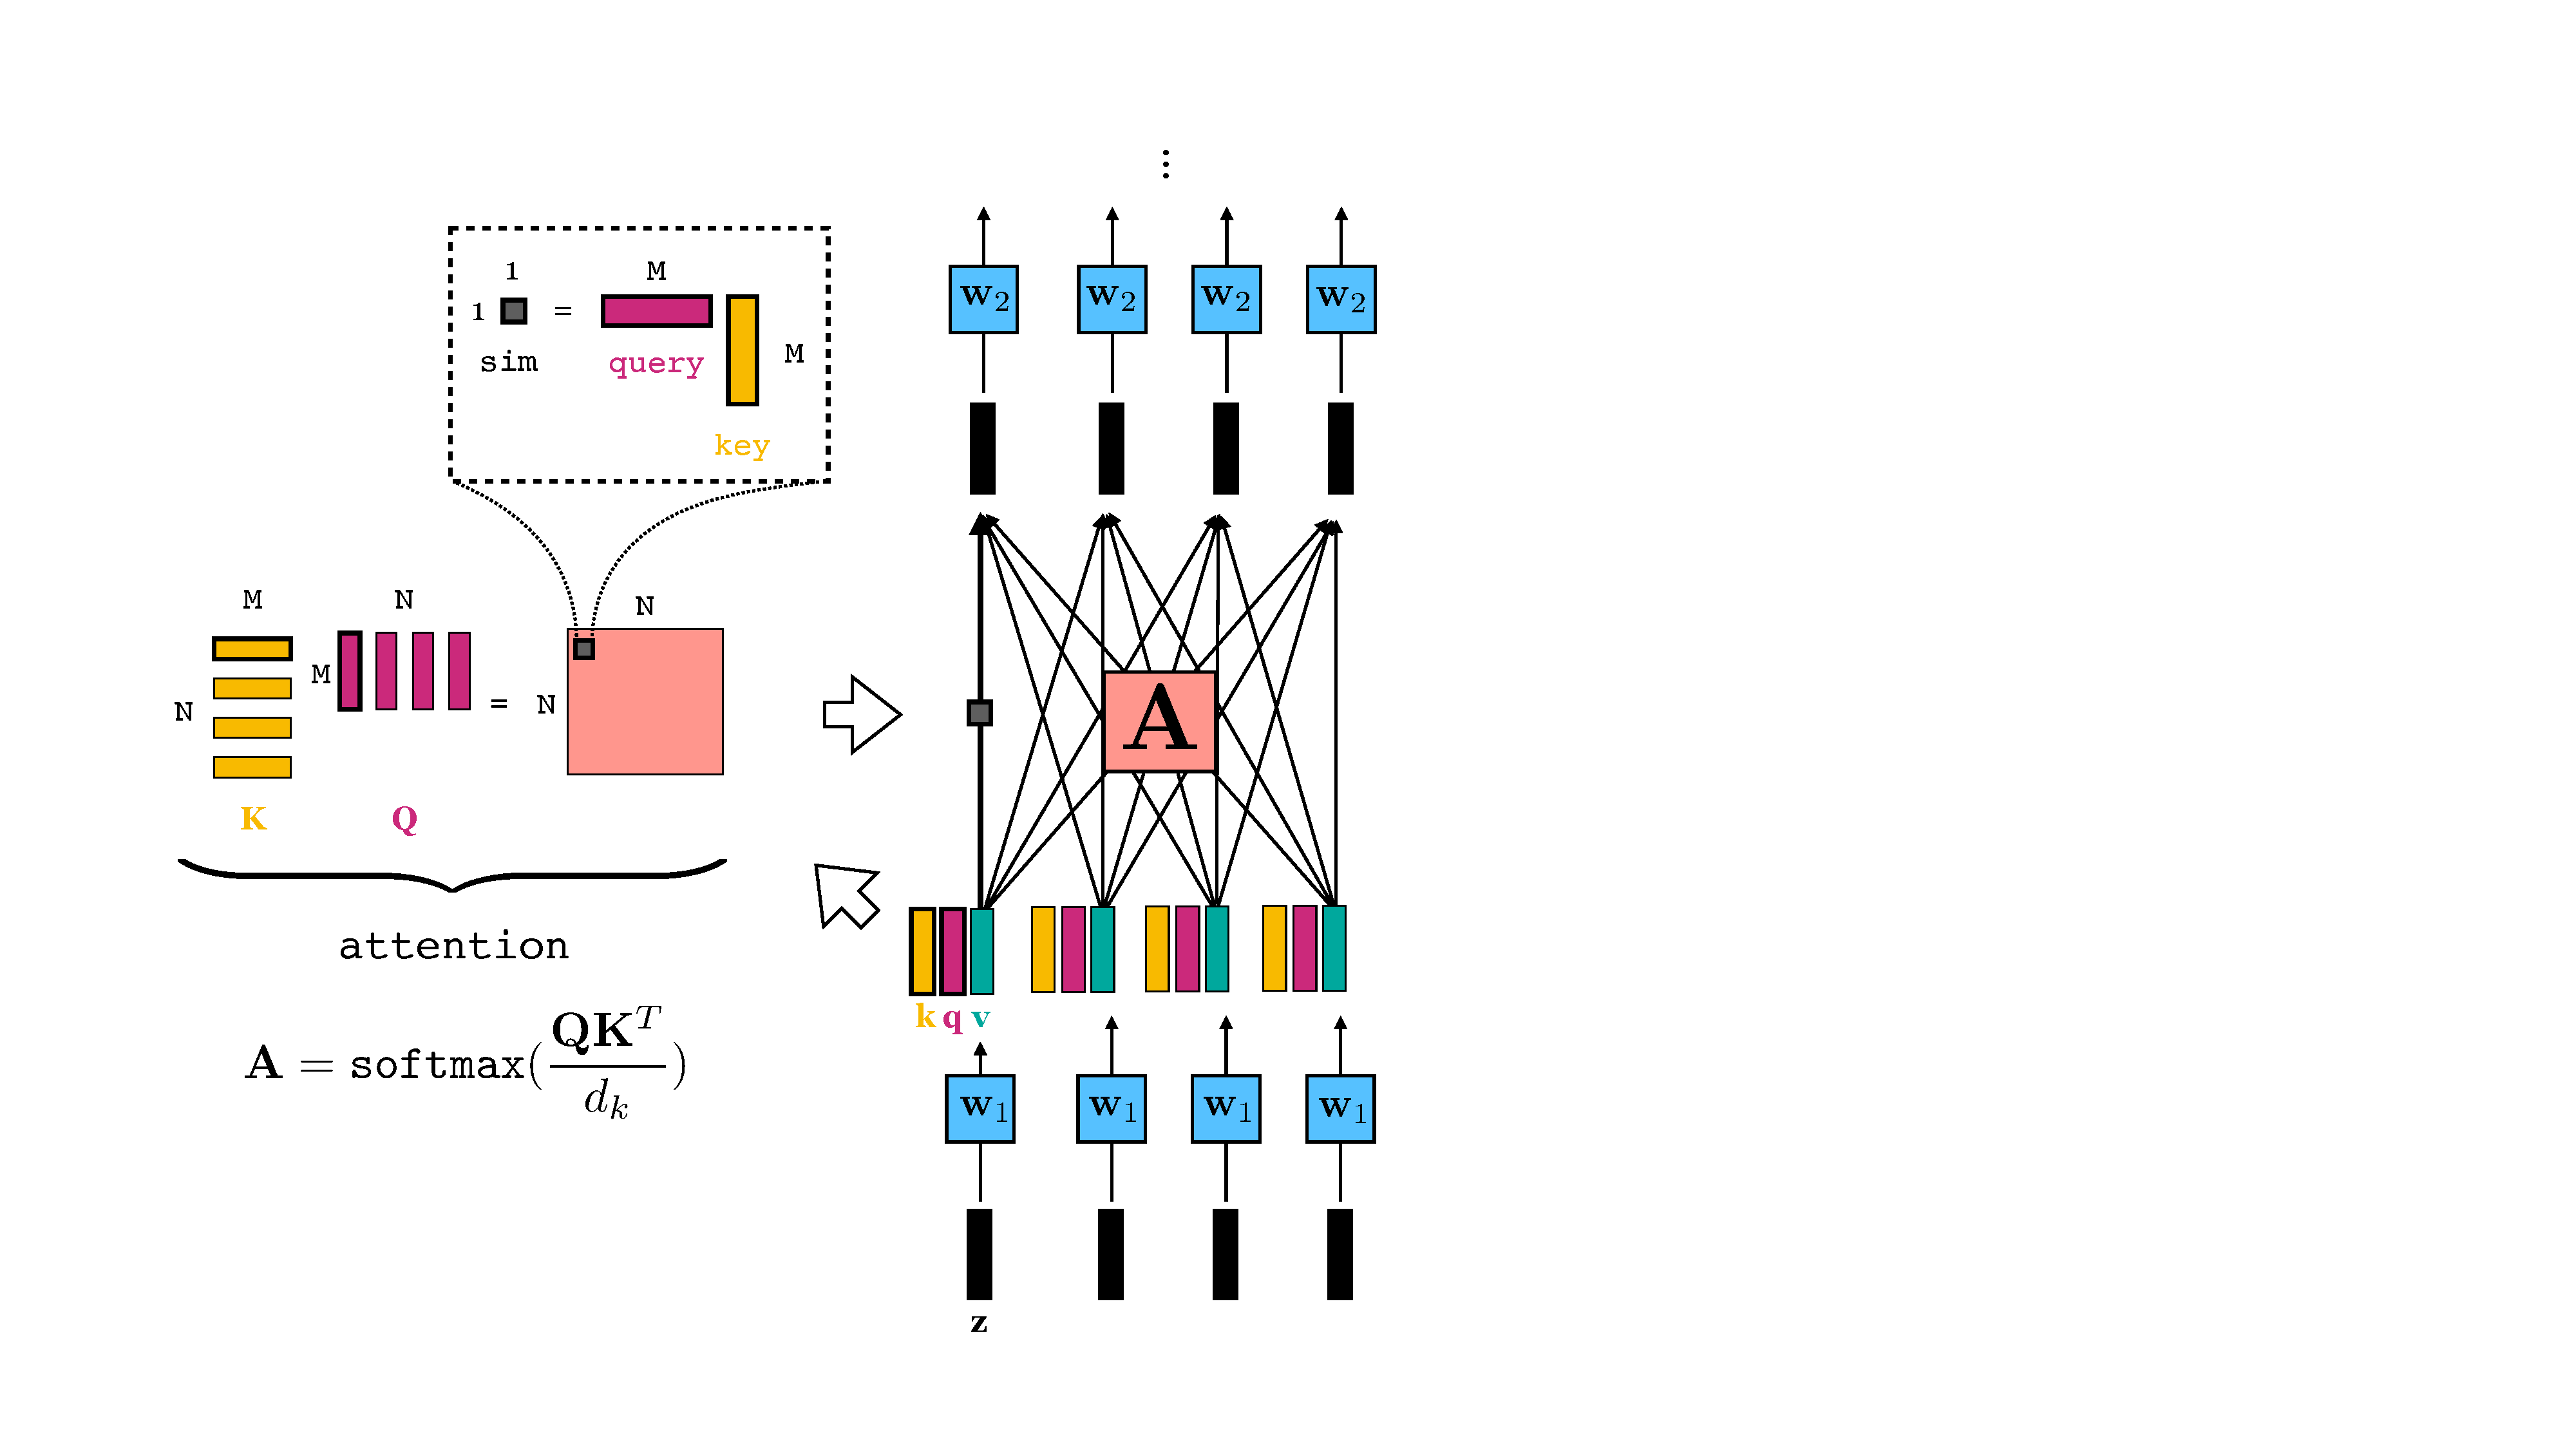
\includegraphics[width=0.6\linewidth]{./figures/transformers/attn_arch.pdf}
%     \label{fig:transformers:attn_arch}
% \end{figure}

This fully defines a self-attention layer, which is the kind of attention layer used in transformers. Before we move on though, let's think through the intuition of what self-attention might be doing.

Consider that we are processing the safari image, and our task is semantic segmentation (label each patch with an object class). Figure \ref{fig:attention_layer_cartoon} illustrates this scenario. We start by tokenizing the image so that each patch is represented by a token. Now we have a token, $\mathbf{t}_2$, that represents the patch of pixels around the torso of the impala. We wish to update this token via one layer of self-attention. Since the goal of the network is to classify patches, it would make sense to update $\mathbf{t}_2$ to get a better semantic representation of what's going on in that patch. One way to do this would be to attend to the tokens representing other patches of the impala, and use them to refine $\mathbf{t}_2$ into a more abstracted token vector, capturing the label \textit{impala}. The intuition is that it's easier to recognize a patch given the context of other relevant patches around it. The refinement operation is just to sum over the token code vectors, which has the effect of reducing noise that is not shared between the three attended impala patches, which amplifies the commonality between them -- the label \textit{impala}. More sophisticated refinements could be achieved via multiple layers of self-attention. Further, the impala patch query could also retrieve information from the giraffe and zebra patches, as those patches provide additional context that could be informative (the animal in the query is more likely to be an impala if it is found near giraffes and zebras, since all those animals tend to congregate together in the same biome).

\begin{figure}[h!]
    \centerline{
        \begin{tikzpicture}
            \draw (0, 0) node[inner sep=0] {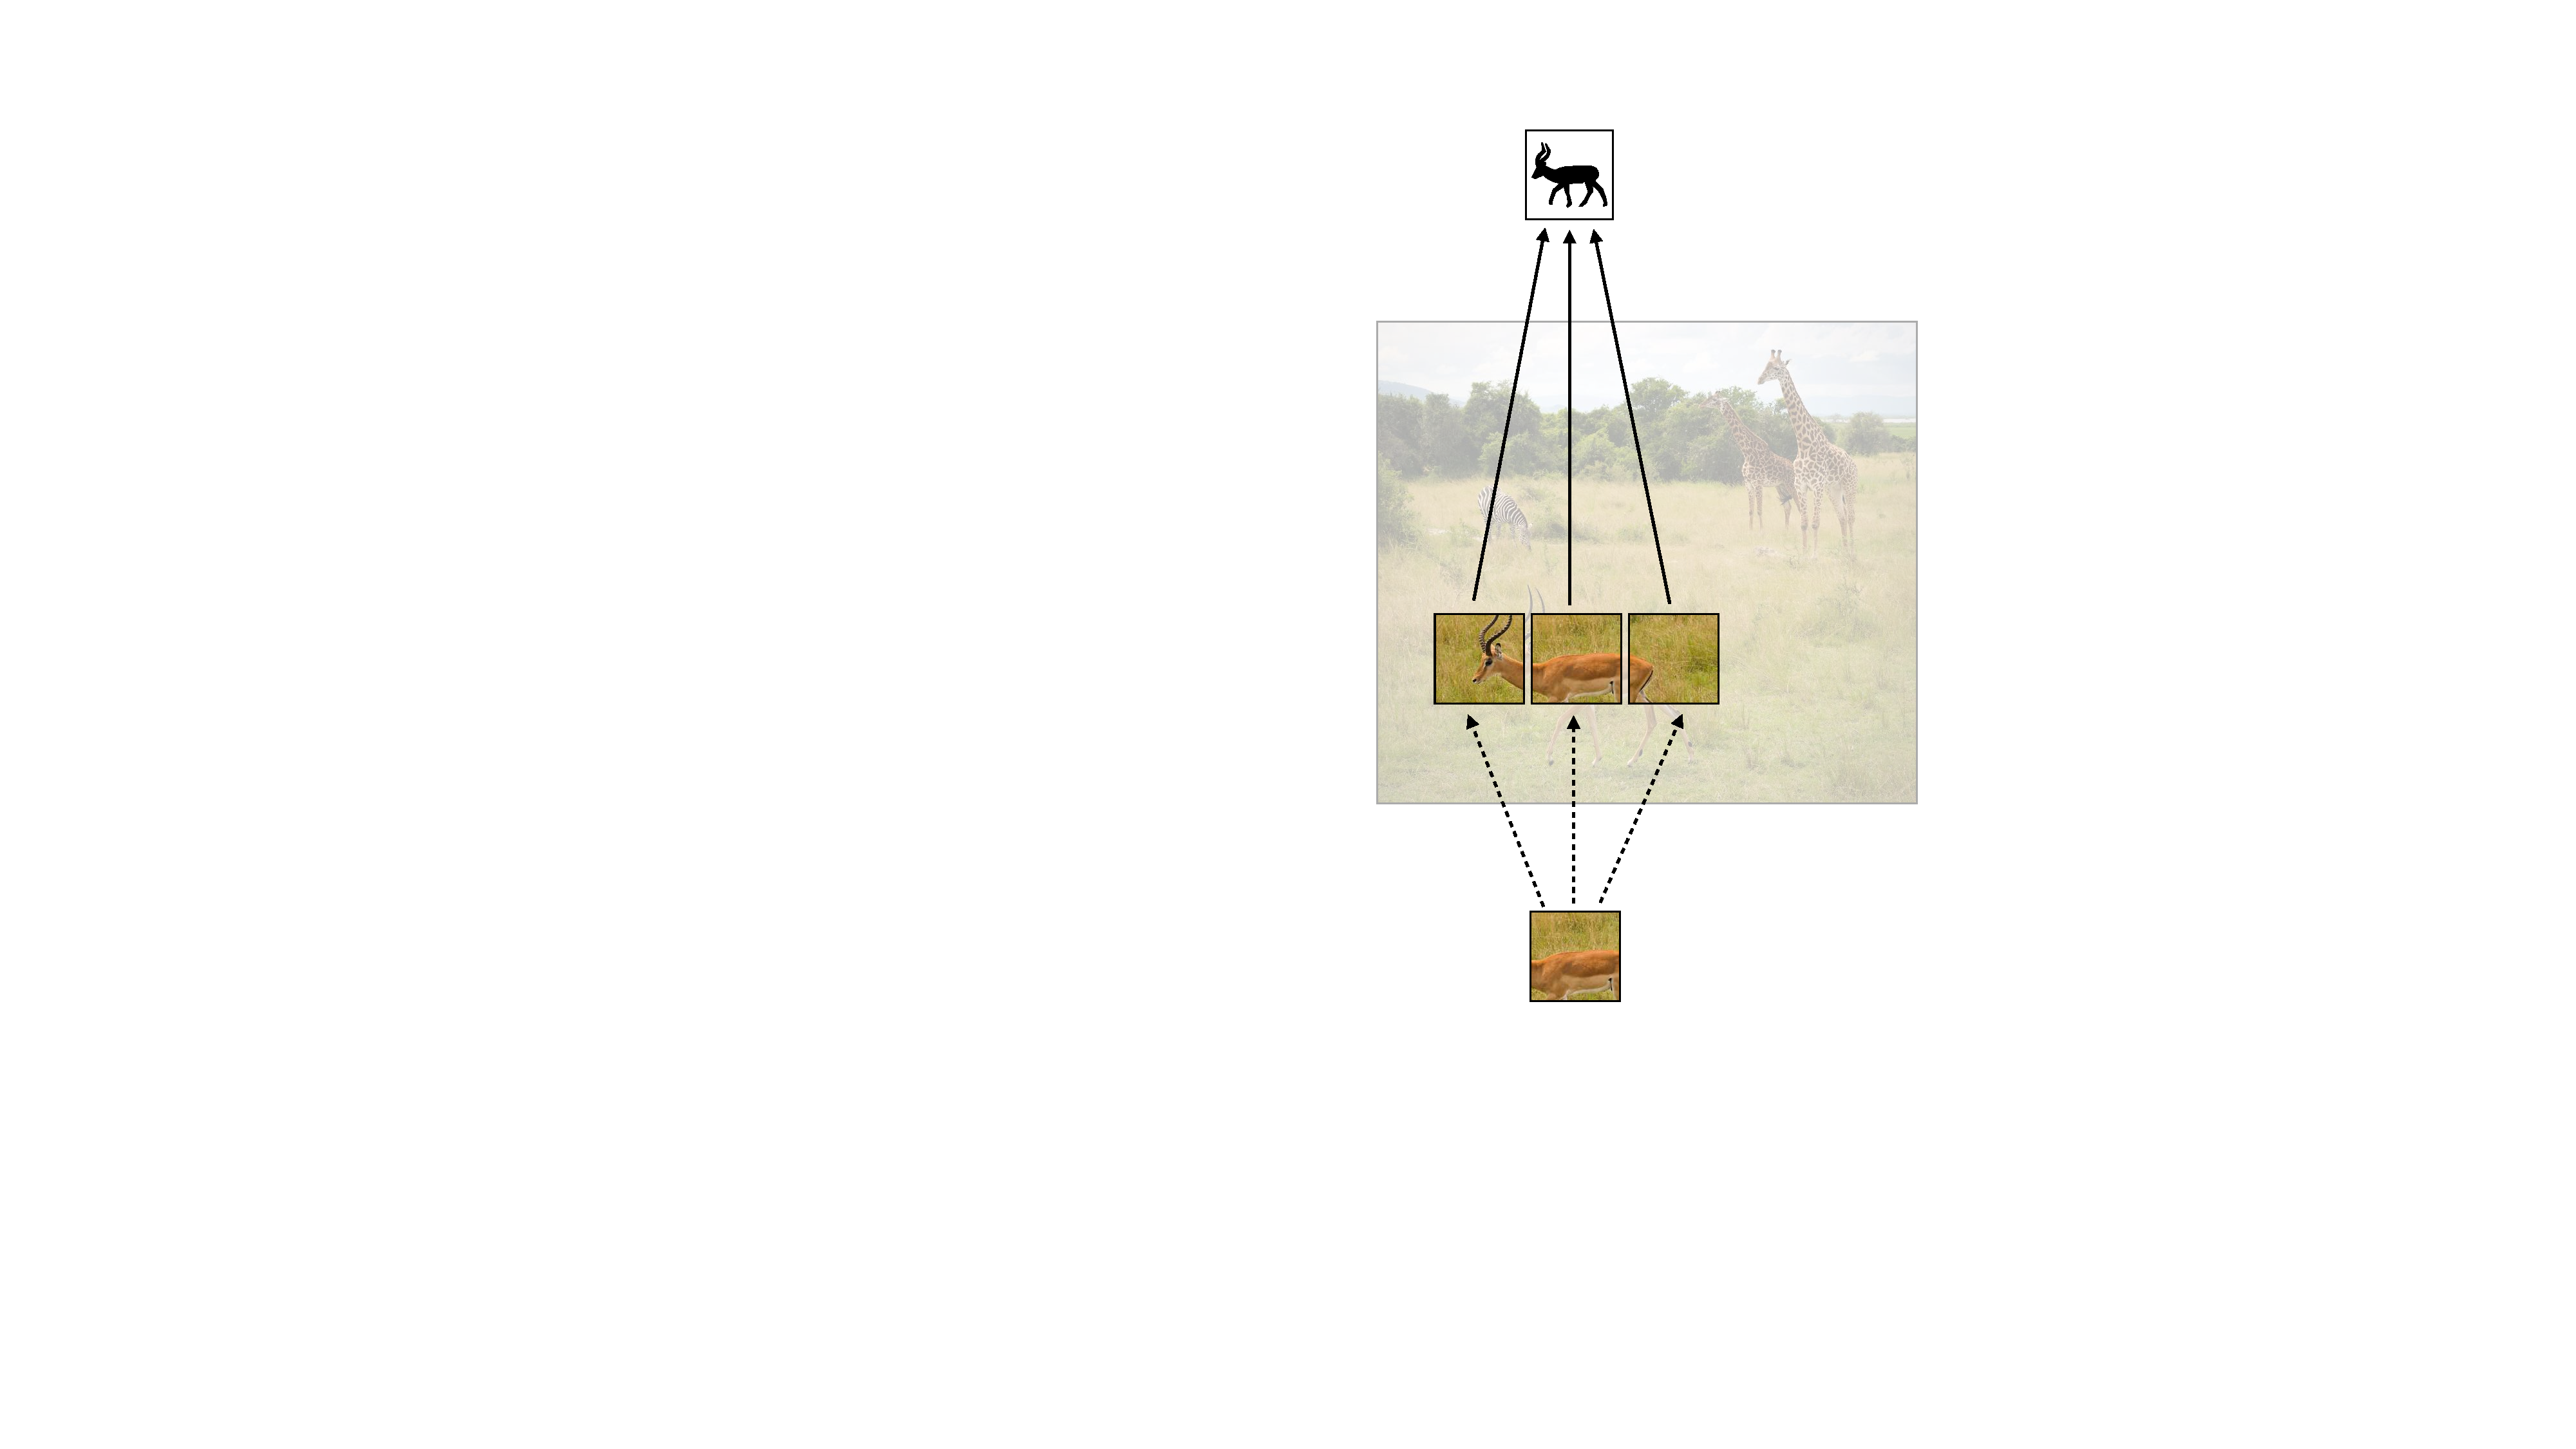
\includegraphics[width=0.38\linewidth]{./figures/transformers/attention_layer_cartoon_safari.pdf}};
            \draw (-0.75, -3.55) node [draw,rectangle,fill=white] {$\mathbf{t}_2$};
            \draw (-0.75, -0.5) node [draw,rectangle,fill=white] {$\mathbf{t}_2$};
            \draw (-0.8, 4.55) node [draw,rectangle,fill=white] {$\mathbf{t}_2$};
            \draw (0.25, -0.5) node [draw,rectangle,fill=white] {$\mathbf{t}_1$};
            \draw (-1.75, -0.5) node [draw,rectangle,fill=white] {$\mathbf{t}_3$};
            \draw (1.25,-2.0) node {\texttt{attention}};
            \draw (0.2,2.2) node {\texttt{sum}};
        \end{tikzpicture}
    }
    \caption{One way self-attention could be used to aggregate information across all patches containing the same object, and thereby arrive at a better representation of the object in $\mathbf{t}_2$, the query patch.}
    \label{fig:attention_layer_cartoon}
\end{figure}

This is just one way self-attention could be used by the network. How it is actually used will be determined by the training data and task. What really happens might deviate from our intuitive story: tokens on hidden layers do not necessarily represent spatially localized patches of pixels. While the initial tokenization layer creates tokens out of local image patches, after this point attention layers can mix information across spatially distant tokens; note that $\toutOne$ does not necessarily represent the same spatial region in the image as $\tinOne$.

\Fig{\ref{fig:transformers:transformers_attn_ex}} gives an example of what self-attention maps can look like on the safari image. In this example, we are simply using patch color as the query and key features. Each attention map shows one row of $\mathbf{A}$ reshaped into the size of the input image.


\begin{figure}
    \centerline{
        \begin{tikzpicture}
            \draw (0, 0) node[inner sep=0] {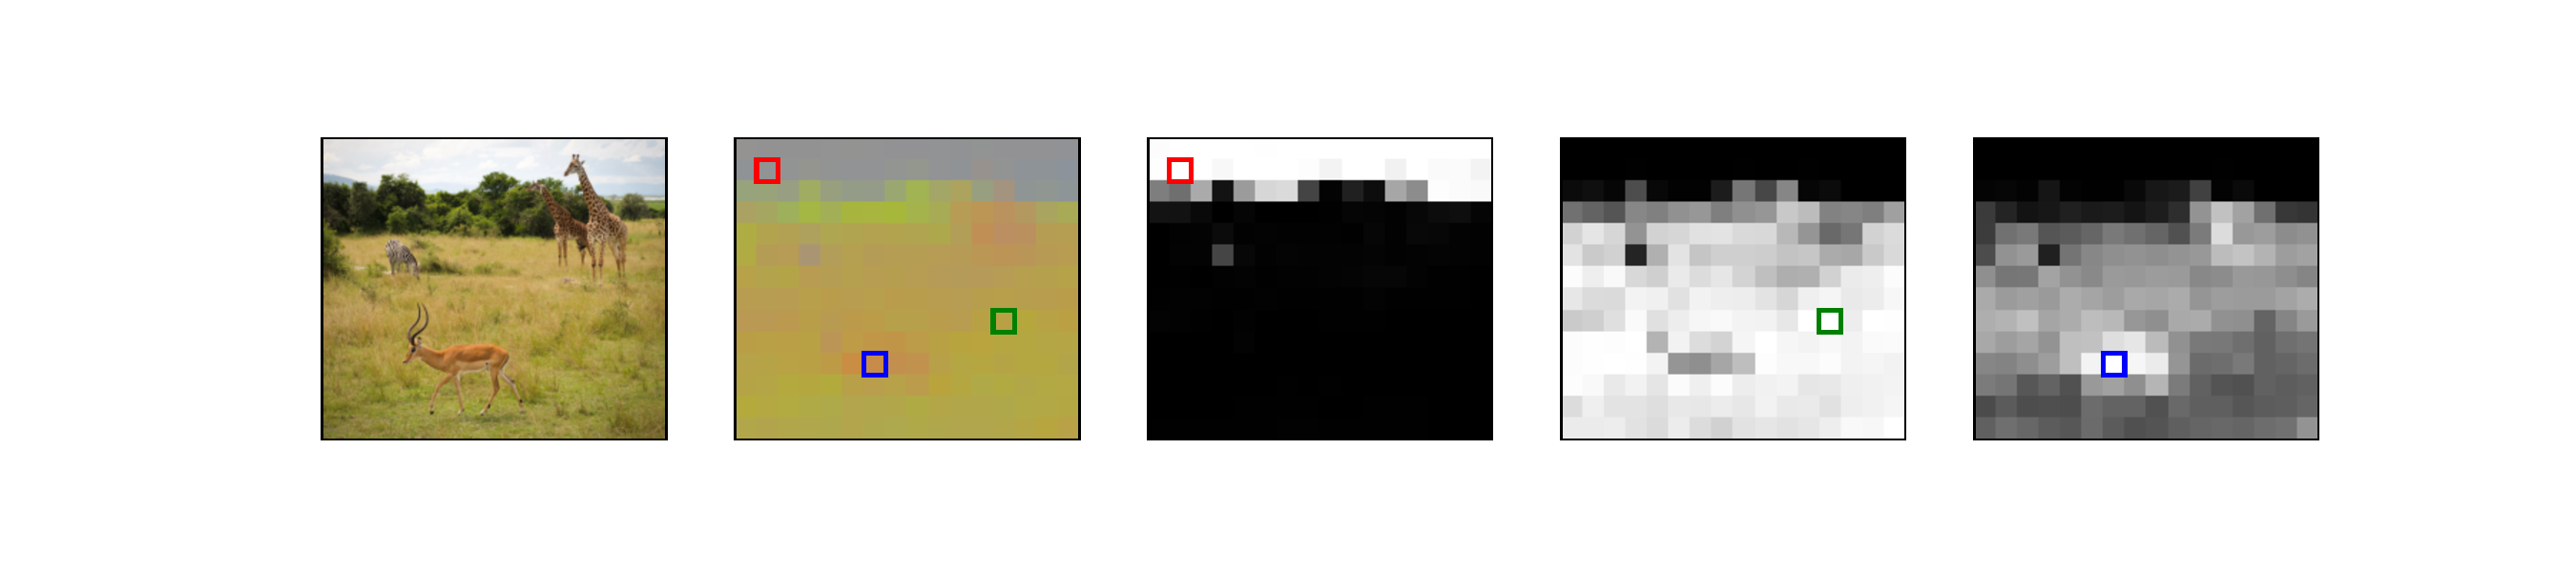
\includegraphics[width=1.0\linewidth]{./figures/transformers/transformers_attn_ex.pdf}};
            \draw (-6.3,1.4) node {\small{input}};
            \draw (-3.2,1.4) node {\small{query/key features}};
            \draw (0,1.8) node {\small{attn map for}}; \draw (0,1.4) node {\small{outlined query}};
            \draw (3.2,1.8) node {\small{attn map for}}; \draw (3.2,1.4) node {\small{outlined query}};
            \draw (6.3,1.8) node {\small{attn map for}}; \draw (6.3,1.4) node {\small{outlined query}};
        \end{tikzpicture}
    }
    \caption{Example of self-attention maps where each token is an image patch and the query and key vectors are both set to the mean color of the patch, normalized to be a unit vector.}
    \label{fig:transformers:transformers_attn_ex}
\end{figure}

%To do so, $t_1$ may allocate attention over other regions of the image that it deems are relevant to understanding the bird's head. Since there are three birds, it would make sense for the $t_1$ to attend to the tokens that represent the other heads. This way it could aggregate the information 

%The way $t_1$ uses its attention is simply to take a weighted sum over the tokens it is attending to. This sum is a summary of all the information being attended to. $t_1$ will then update its code by adding in this weighted sum over the codes of all the tokens it is attending to.


% Let's consider just one token in the input; the steps we describe next will be applied to each token in the same way. To anthropomorphize for a minute, the token's goal is to improve it's representation by mixing in information from the other tokens in the input. The token first \textbf{queries} the other tokens, asking ``which of you match my query". The query is vector output as a function of the token's internal vector. The query vector is matched against the \textbf{key} vector of each token in the input vector of tokens. The best matching tokens submit a response as a \textbf{value} vector to be averaged into the querier's internal vector.

% We will create a matrix $\mathbf{S}$ of the similarity between $\mathbf{q}_{t}$ and $\mathbf{k}_{t_{\texttt{in}_i}}$ for all tokens $t_{\texttt{in}_i}$:
% \begin{align}
%     \mathbf{S}_i = \texttt{sim}(\mathbf{q}_{t}, \mathbf{k}_{t_{\texttt{in}_i}})
% \end{align}




% \begin{align}
%     t_1 \leftarrow w_1 t_1 + w_2 t_2 + w_3 t_3
% \end{align}

%\textbf{Attention layers} can be easily understood by starting with the linear combination of tokens defined above. An attention layer is simply an linear layer whose weights are determined as \textit{functions of the data}. The intuition is that this function decides what parts of the input to ``attend" to in producing the output representation. 

%If a weight between an input and output token is near-zero, then that input is ignored; if the weight is high then that input is attended to.



% \begin{figure}[h]
%     \centering
%     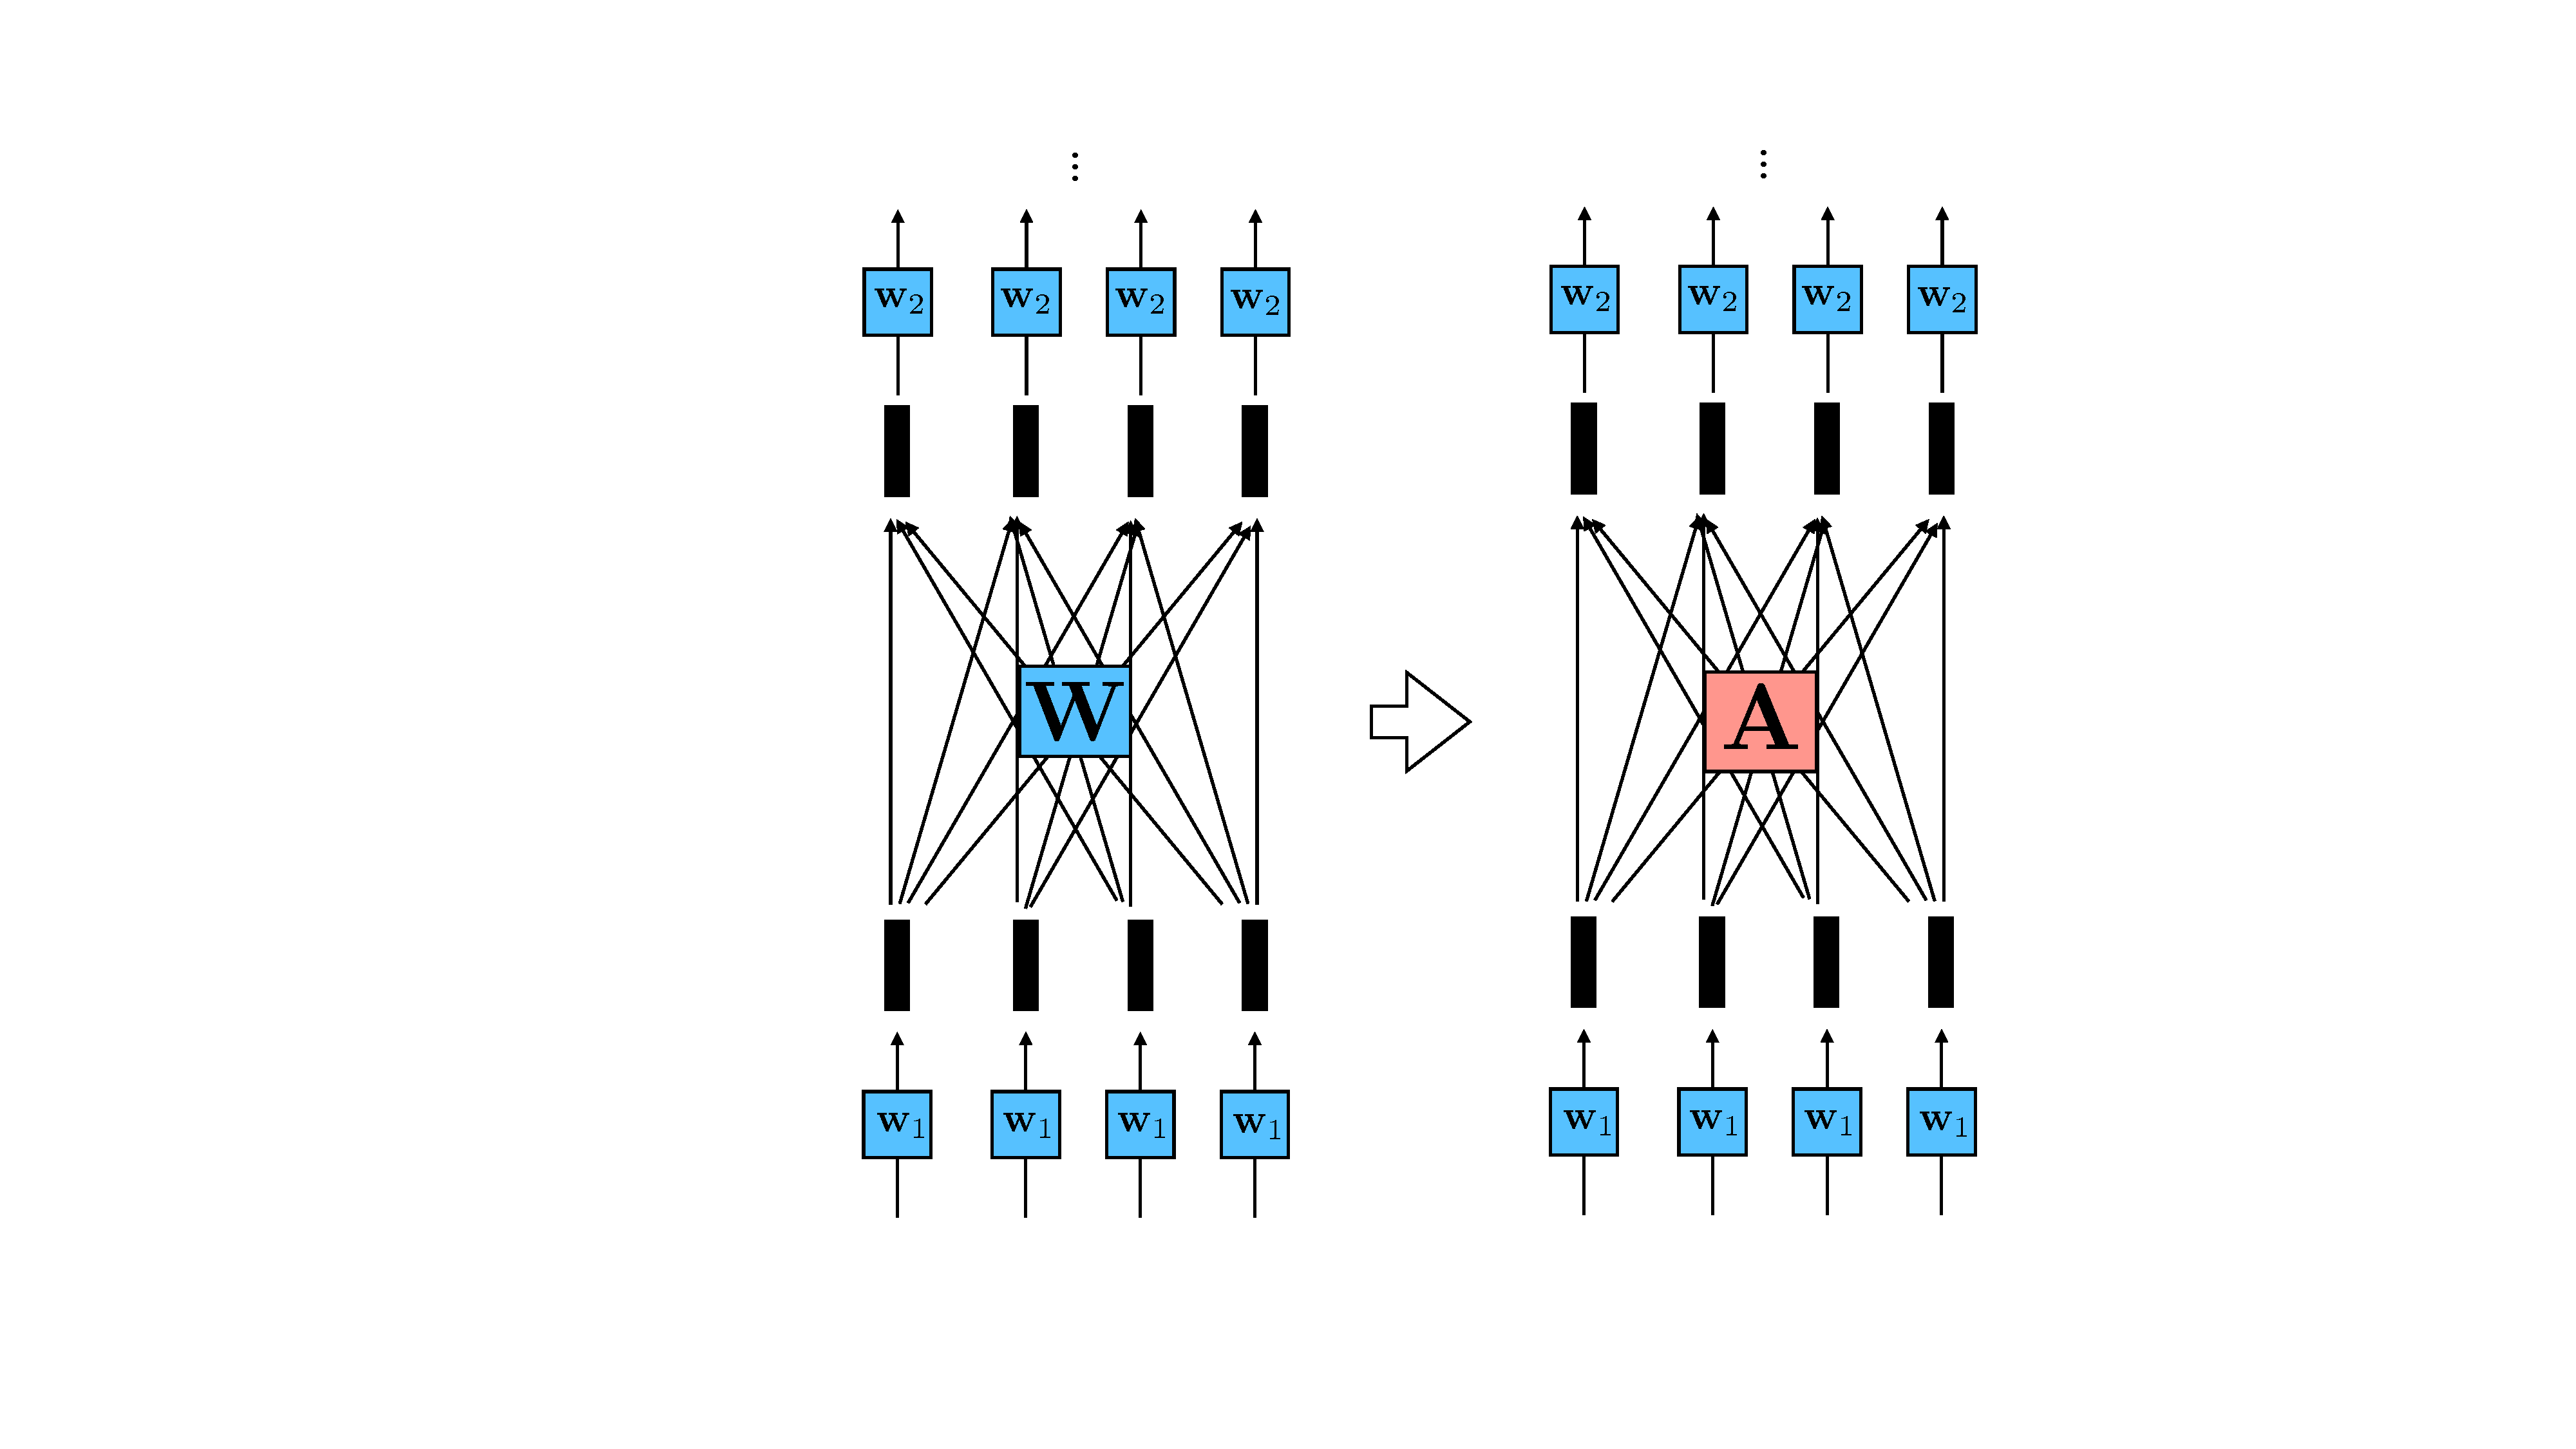
\includegraphics[width=0.6\linewidth]{./figures/transformers/fc_to_attn.pdf}
%     \label{fig:transformers:fc_to_attn}
% \end{figure}

%Rather than applying \textit{the same} filter to different locations in a signal, transformers apply a \textit{dynamic filter} that is different at each different location. However, the dynamics that determine the filter weights \textit{are the same} across locations! So we have something like Property \#2 of CNNs (see Chapter XX), except at an abstracted level: the weights are not shared but how the weights are determined is shared.

%The workhorse of transformers is {\bf self-attention layers}. These layers take a set of {\bf tokens} as input and produce a transformed set of tokens as output. A ``token" is simply transformer lingo for a vector. The set of tokens need not have any ordering -- all the computations over tokens can occur in parallel. Just like with ``patches" in a CNN, each token is processed in a manner that is independent and identical to how all the other tokens are processed.

% You are probably wondering: what is $f$ in the figure above? Well, since $\mathbf{A}$ is not free parameters, its value has to be some other way. What we have depicted above is \textbf{self-attention} where $\mathbf{A}$ is determined by a function $f$ of the \textit{inputs to the attention layer themselves}:
% \begin{align}
%     \mathbf{A} &= f(\tin, \ldots)  \quad\quad \triangleleft \text{ self-attention}\\
%     \Xout &= \mathbf{A}\tin
% \end{align}

% Transformers use self-attention layers like this. In general, however, the attention weights $\mathbf{A}$ could be determined in other ways, for example, an external signal or a separate branch of the computation graph could be the inputs to $f$ that determines $\mathbf{A}$. In general, an attention layer can be any linear layer where the \textit{weights} are \textit{data-dependent}, that is, they are determined as the \textit{output activations} of data processing by some other module of the computation graph\marginnote{In this way, the parameters of the net $\mathbf{A}$ are the outputs of another net $f$. A net that parameterizes another net is sometimes called a hypernet~\cite{XX}, so attention is a hypernet~\cite{XX}.}[-0.4cm]:
% \begin{align}
%     \mathbf{A} &= f(\ldots) \quad\quad \triangleleft \text{ attention}\\
%     \Xout &= \mathbf{A}\tin
% \end{align}
% The interesting thing about attention is that it mixes the concepts of weights and activations, which previously we had kept separate.

% \subsection{Query-Key-Value attention}
% Transformers use a particular kind of self-attention based on the idea of keys, queries, and values from the information retrieval literature.

% Let's consider just one token in the input; the steps we describe next will be applied to each token in the same way. To anthropomorphize for a minute, the token's goal is to improve it's representation by mixing in information from the other tokens in the input. The token first \textbf{queries} the other tokens, asking ``which of you match my query". The query is vector output as a function of the token's internal vector. The query vector is matched against the \textbf{key} vector of each token in the input vector of tokens. The best matchig tokens submit a respose as a \textbf{value} vector to be averaged into the querier's internal vector.
% \begin{figure}
%     \centering
%     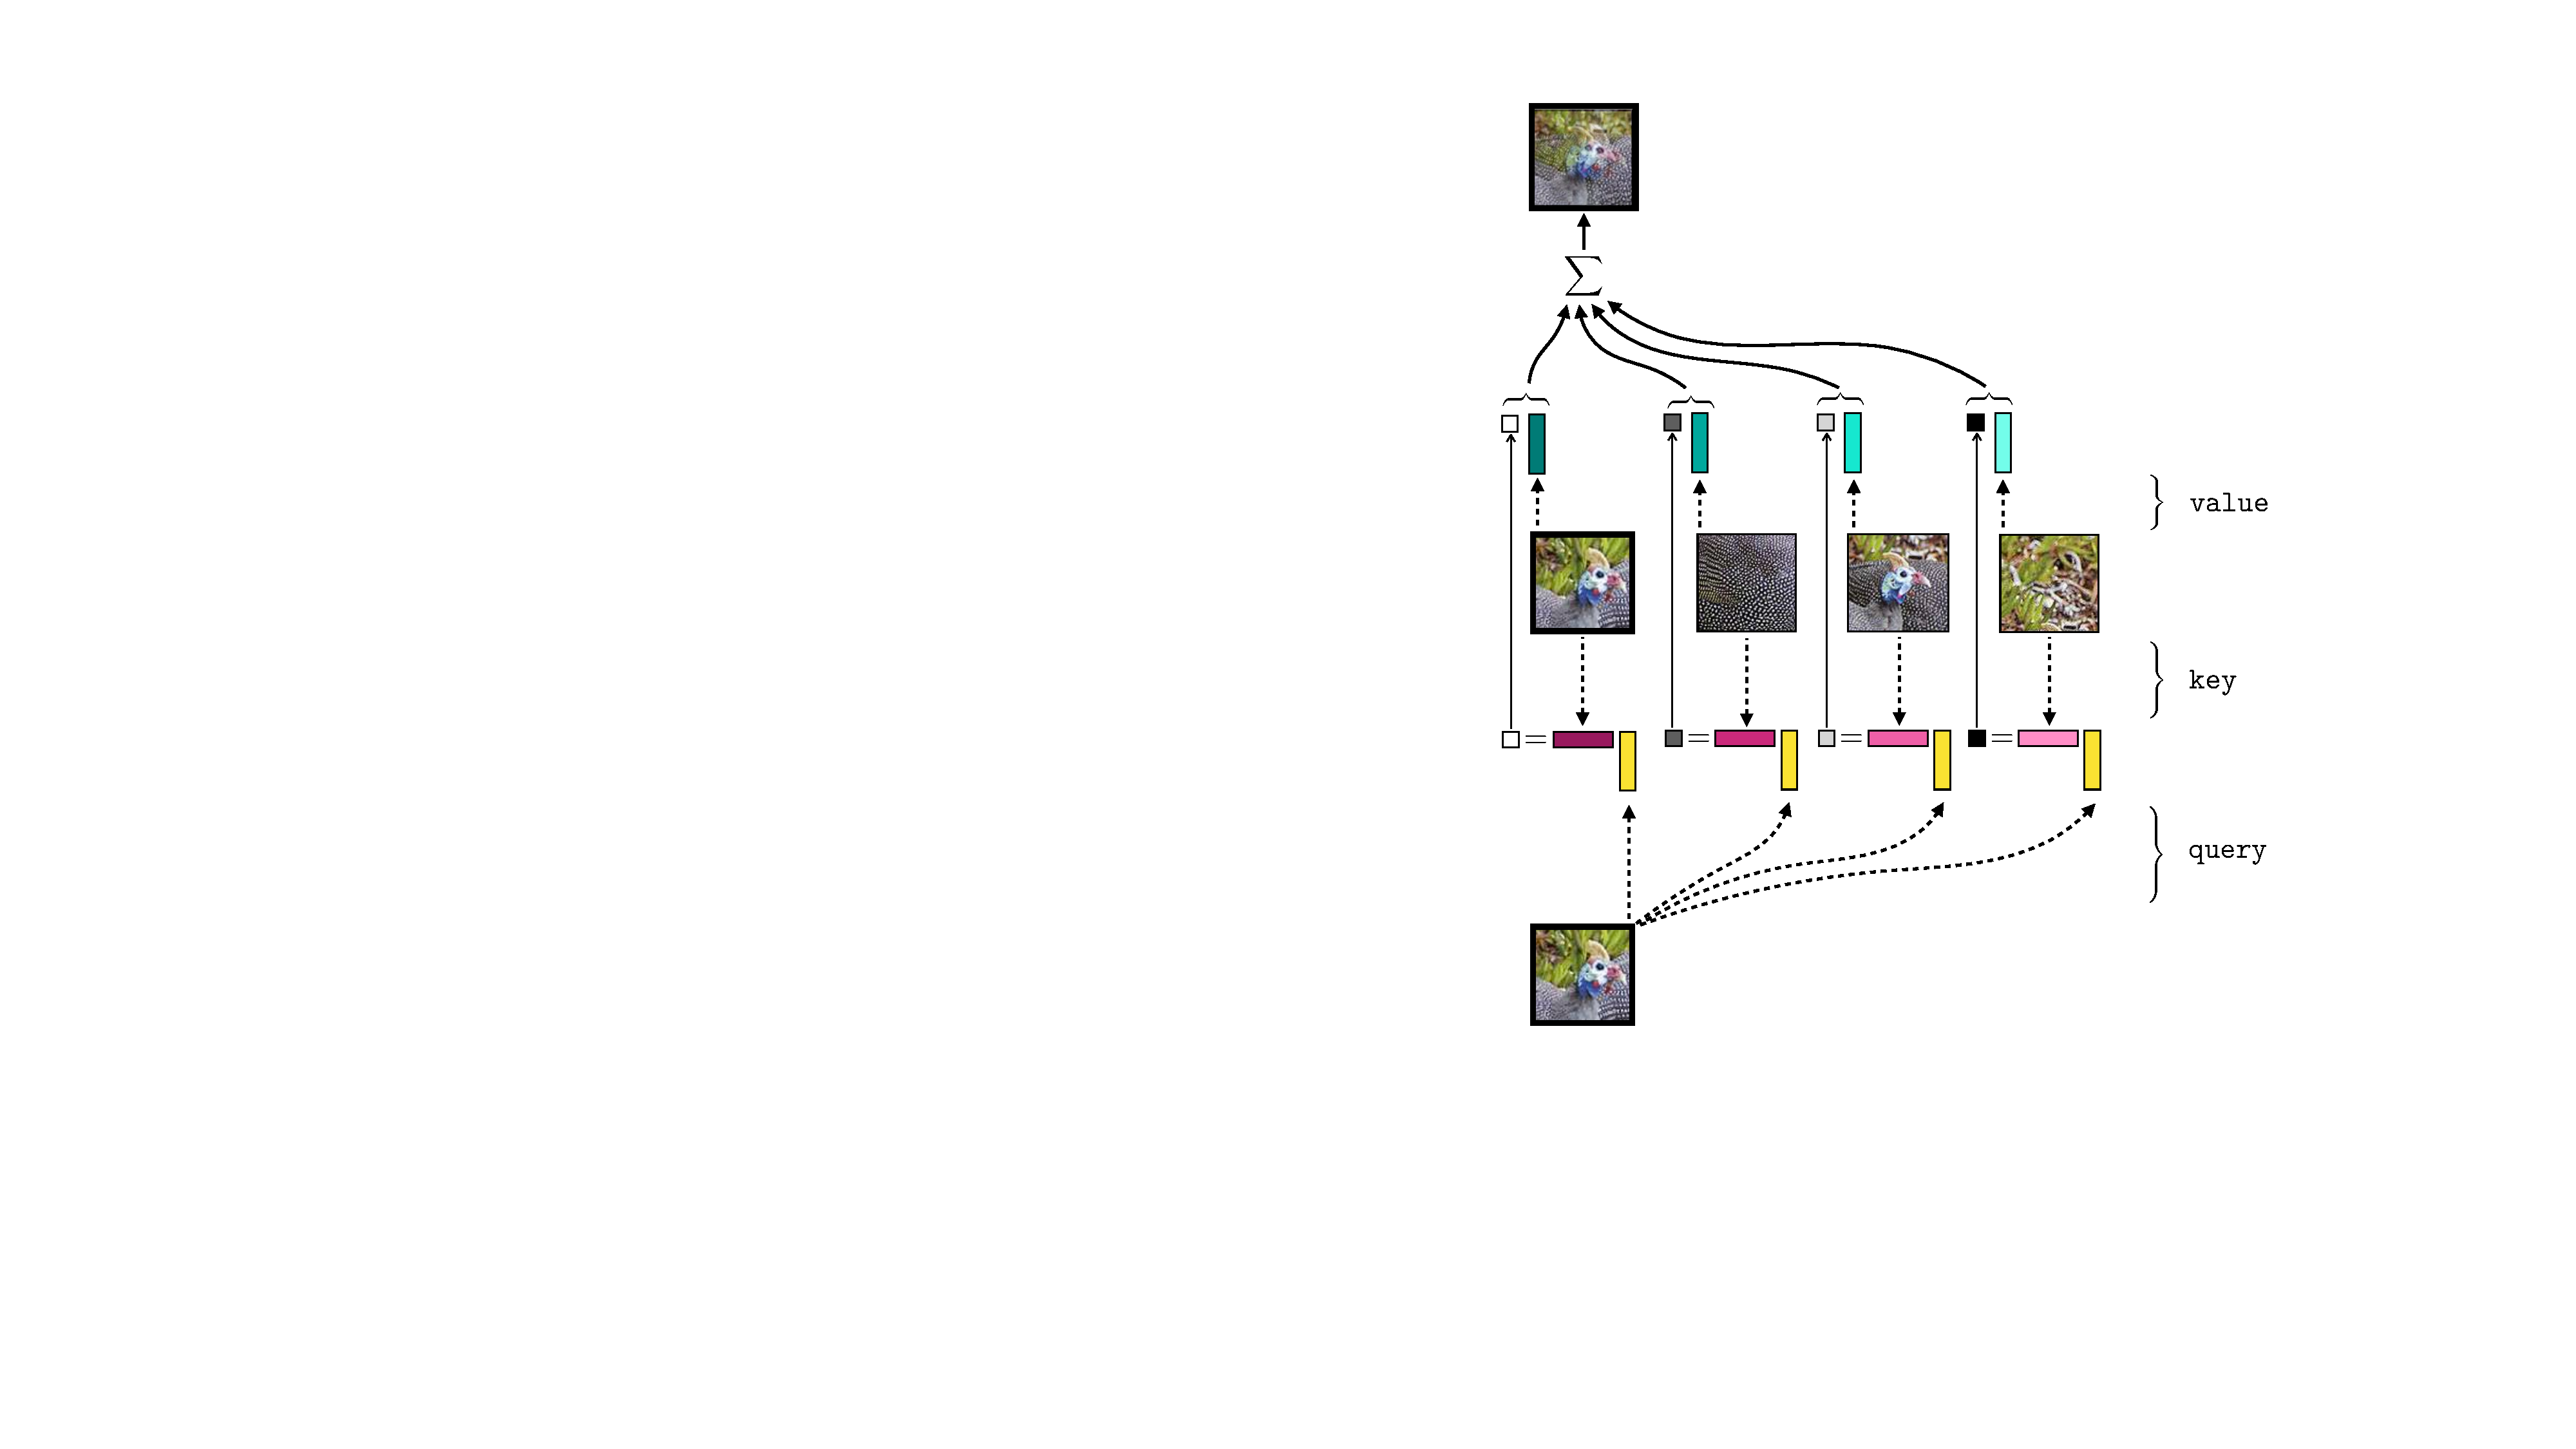
\includegraphics[width=0.5\linewidth]{./figures/transformers/attention_layer_1_token.pdf}
%     \label{fig:attention_layer_1_token}
% \end{figure}


% To motivate self-attention, we will start with a stripped down version. 
% %Let $\Xin \in \mathbb{R}^{N \times M}$ denote $N$ input tokens each of which is a $1 \times M$ dimensional vector. $\Xout$ is the corresponding array of transformed output tokens. Then a simple kind of self-attention layer can be defined by the following operations:
% Suppose we have a vector of tokens, $\tin$ as input to our self-attention layer. First, we measure the similarity between each token in the vector and every other token in the vector. Our notion of similarity between two tokens will be their inner product. Using our notation for tokens, the matrix of all the inner products between the input tokens can be compactly written as an outer-product:
% \begin{align}
%     %\mathbf{G} &= \Xin\Xin^T\\
%     \mathbf{G} &= \tin\tin^T
% \end{align}
% %$\mathbf{G}$$ is a \textbf{Gram matrix} -- a matrix of inner products between all elements in a vector.
% $\mathbf{G}$ is the Gram matrix over tokens; it measures the similarity (dot product) between all pairs of tokens. We will use this similarity matrix to determine the amount of ``attention" each token pays to each other token. 

% We want to use these values to decide how much attention each token should pay to each other token. Intuitively, we want the amount of total attention to be a constant value and the weights to be nonnegative, so we will pass $\mathbf{G}$ through a softmax to obtain our affinity matrix $\mathbf{A}$:
% \begin{align}
%     \mathbf{A} &= \texttt{softmax}(\mathbf{G})\Y \quad\quad \triangleleft \text{ softmax over rows}\\
%     \tout &= \mathbf{A}\tin
% \end{align}



% If we then pass each row of $\mathbf{G}$ through a $\texttt{softmax}$ function then we can interpret each softmaxed row as a normalized set of non-negative weights that we will use in a weighted sum over tokens, i.e. our affinity matrix $\mathbf{A}$. Finally we compute this weighted sum as $\tout = \mathbf{A}\tin$. The output tokens are weighted sums of the input tokens, weighted by the similarity of each input token with each other input token. This layer will act to cluster the tokens since similar tokens end up being averaged together and that results in them becoming more similar to each other.

% We will make this clearer graphically. We will focus on how the self-attention layer updates just one token, $\xin \rightarrow \xout$:


% \begin{figure}[h]
% \centering
% \begin{tikzpicture}
%     \def\neuronrad{0.35}
%     \draw [fill=blue] (0,0) rectangle ++(\neuronrad/2,\neuronrad*2);
%     %
%     \draw (0,1) node {$\xout = \sum_{i=1}^N a_i \Xin[i,:]$}
% \end{tikzpicture}
% \end{figure}

% If we want to do more than just clustering, we can introduce additional transformations, which will yield the canonical self-attention layers used in transformers.
% \begin{align}
%     \mathbf{Q} &= \Xin\mathbf{W}^q &\triangleleft \quad\quad \texttt{query}\\
%     \mathbf{K} &= \Xin\mathbf{W}^k &\triangleleft \quad\quad \texttt{key}\\
%     \mathbf{V} &= \Xin\mathbf{W}^v &\triangleleft \quad\quad \texttt{value}\\
%     \Xout &= \texttt{softmax}(\frac{\mathbf{Q}\mathbf{K}^T}{d_k})\mathbf{V}
% \end{align}
% Notice that $\Xin\mathbf{W}^q = \sum_{c=1}^C \mathbf{W}^q_{k,c} \star \mathbf{X}_{\texttt{in}_c}$, which, referring back to Chapter \ref{chapter:convolutional_neural_nets} can be identified as a multi-channel convolution layer (without a bias). This reveals a connection between transformers and CNNs: the query, key, and value in transformers is arrived at by convolving the input set of tokens with a learned set of filters (the convolution kernels in this case are $1 \times 1$ in the ``spatial", cross-token, domain). All these operations happen independently and identically at the token level. Then the attention matrix is just a linear layer on top. This linear layer is data dependent because its weights are constructed from the tokens. %That data-dependency shares a property with an RNN: it can model bilinear dependencies over signals of unbounded length, whereas CNNs can only model local dependencies.

%\subsection{Multi-headed attention}

%The transformer encoder blocks defined in \cite{vaswani2017attention} operate as follows:
%\begin{align}
%    \texttt{MSH}(\Xin)
%\end{align}

\subsection{Multihead Self-Attention}
Despite their power, self-attention layers are still limited in that they only have one set of query/key/value projection matrices (namely, $\mathbf{W}_q$, $\mathbf{W}_k$, $\mathbf{W}_v$). These matrices define the notion of similarity that is used to match queries to keys. In particular, the similarity between two tokens $i$ and $j$ is measured as:
\begin{align}
    s_{ij} & = \mathbf{q}_i^\transpose \mathbf{k}_j                                     \\
           & = (\mathbf{W}_q \mathbf{t}_i)^\transpose \mathbf{W}_k \mathbf{t}_j         \\
           & = \mathbf{t}_i^\transpose\mathbf{W}_q^\transpose \mathbf{W}_k \mathbf{t}_j \\
           & = \mathbf{t}_i^\transpose\mathbf{S}\mathbf{t}_j
\end{align}
What this shows is that $\mathbf{W}_q$ and $\mathbf{W}_k$ define some matrix $\mathbf{S} = \mathbf{W}_q^\transpose \mathbf{W}_k$ that modulates how we measure similarity (dot product) between $\mathbf{t}_i$ and $\mathbf{t}_j$. A single self-attention layer therefore measures similarity in just one way.

What if we want to measure similarity in more than one way? For example, maybe we want our net to perform some set of computations based on color similarity, another based on texture similarity, and yet another based on shape similarity? The way transformers can do this is with \index{Attention!Multihead self-attention}\textbf{multihead self-attention} (\textbf{MSA}). This method simply consists of running $k$ attention layers in parallel. All these layers are applied to the same input $\tin$. This results in $k$ output sets of tokens, $\tout^1, \ldots, \tout^k$. To merge these outputs, we concatenate all of them and project back to the original dimensionality of $\tin$. These steps are shown in the math below:
\begin{align}
    \tout^i                         & = \texttt{attn}^i(\tin) \quad \text{for } i \in \{1,\ldots,k\}                                                                                                                            \\
    \bar{\mathbf{T}}_{\texttt{out}} & = \begin{bmatrix}
                                            \tout^1[0,:]   & \ldots & \tout^k[0,:]   \\
                                            \vdots         & \vdots & \vdots         \\
                                            \tout^1[N-1,:] & \ldots & \tout^k[N-1,:] \\
                                        \end{bmatrix}                    & \quad\quad \triangleleft \quad \bar{\mathbf{T}}_{\texttt{out}} \in \mathbb{R}^{N \times kv}                                                          \\
    \tout                           & = \bar{\mathbf{T}}_{\texttt{out}}\mathbf{W}_{\texttt{MSA}}     & \quad\quad \triangleleft \quad \mathbf{W}_{\texttt{MSA}} \in \mathbb{R}^{kv \times d} \label{eqn:transformers:MSA_merge}
\end{align}
where $v$ is the dimensionality of the value vectors and $d$ is the dimensionality of the code vectors of the output (\cite{dosovitskiy2020vit} recommends setting $kv = d$). The matrix $\mathbf{W}_{\texttt{MSA}}$ \textit{merges} all the heads; its values are learnable parameters. The other learnable parameters of MSA are the query, key, and value projections for each of the $k$ attention heads.
\marginnote{Notice that here, unlike in the single-headed self-attention layers presented previously, the value vectors need not have the same dimensionality as the token code vectors, since we are applying the projection \eqn{\ref{eqn:transformers:MSA_merge}}.}[-2.4cm]

The basic reasoning here is quite simple: if self-attention layers are a good thing, why not just add more of them? We can add more \textit{sequential} self-attention layers by building deeper transformers, or we can add more \textit{parallel} self-attention layers by using MSA.

\section{The Full Transformer Architecture}\label{sec:transformers:ViT_arch}

%The transformer architecture consists of a sequence of {\bf transformer encoder} blocks, each of which relies on self-attention layers. Just like a self-attention layer, each transformer encoder takes a set of $N$ tokens as input and produces a set of $N$ tokens as output.

A full transformer architecture is a stack of self-attention layers interleaved with tokenwise nonlinearities. These two steps are analogous to linear layers interleaved with neuronwise nonlinearities in an MLP, as shown below (\fig{\ref{fig:transformers:transformer_vs_MLP}}):
\begin{figure}[h]
    \centerline{
        \begin{minipage}{.49\linewidth}
            \centering
            \begin{tikzpicture}
                %
                \def\Nnodes{3}
                \def\Nlayers{4}
                \def\layerheight{1.2}
                \def\neuronrad{0.1}
                \def\neuronstep{0.7}
                \foreach \x in {1,...,\Nnodes} {
                        \foreach \y in {1,...,\Nlayers} {
                                \draw (\neuronstep*\x,(\layerheight*\y-\layerheight) circle (\neuronrad);
                            }
                    }
                % mixing layer 1
                \foreach \xi in {1,...,\Nnodes} {
                        \foreach \xj in {1,...,\Nnodes} {
                                \draw [thick] [nn_edge] (\neuronstep*\xi,\neuronrad) -- (\neuronstep*\xj,\layerheight-\neuronrad);
                            }
                    }
                % pointwise nonlinearity
                \foreach \x in {1,...,\Nnodes} {
                        \draw [thick] [nn_edge] (\neuronstep*\x,\layerheight+\neuronrad) -- (\neuronstep*\x,\layerheight*2-\neuronrad);
                    }
                % mixing layer 2
                \foreach \xi in {1,...,\Nnodes} {
                        \foreach \xj in {1,...,\Nnodes} {
                                \draw [thick] [nn_edge] (\neuronstep*\xi,\layerheight*2+\neuronrad) -- (\neuronstep*\xj,\layerheight*3-\neuronrad);
                            }
                    }
                %
                \draw (\neuronstep*2,3.7*\layerheight) node {\textbf{MLP}};
                \draw (-0.5,0.5*\layerheight) node {\texttt{linear}};
                \draw (-0.5,1.5*\layerheight) node {\texttt{relu}};
                \draw (-0.5,1.2*\layerheight) node {(neuron-wise)};
                \draw (-0.5,2.5*\layerheight) node {\texttt{linear}};
            \end{tikzpicture}
        \end{minipage}
        \begin{minipage}{.49\linewidth}
            \centering
            \begin{tikzpicture}
                %
                \def\Nnodes{3}
                \def\Nlayers{4}
                \def\layerheight{1.2}
                \def\neuronrad{0.3}
                \def\neuronstep{0.7}
                \foreach \x in {1,...,\Nnodes} {
                        \foreach \y in {1,...,\Nlayers} {
                                \draw (\neuronstep*\x-\neuronrad/4,(\layerheight*\y-\layerheight-\neuronrad) rectangle ++(\neuronrad/2,\neuronrad*2);
                            }
                    }
                % mixing layer 1
                \foreach \xi in {1,...,\Nnodes} {
                        \foreach \xj in {1,...,\Nnodes} {
                                \draw [thick] [nn_edge] (\neuronstep*\xi,\neuronrad) -- (\neuronstep*\xj,\layerheight-\neuronrad);
                            }
                    }
                % pointwise nonlinearity
                \foreach \x in {1,...,\Nnodes} {
                        \draw [thick] [nn_edge] (\neuronstep*\x,\layerheight+\neuronrad) -- (\neuronstep*\x,\layerheight*2-\neuronrad);
                    }
                % mixing layer 2
                \foreach \xi in {1,...,\Nnodes} {
                        \foreach \xj in {1,...,\Nnodes} {
                                \draw [thick] [nn_edge] (\neuronstep*\xi,\layerheight*2+\neuronrad) -- (\neuronstep*\xj,\layerheight*3-\neuronrad);
                            }
                    }
                \draw [thick] [nn_edge] (2.5,0) arc
                    [
                        start angle=-70,
                        end angle=90,
                        x radius=0.4cm,
                        y radius =0.3cm
                    ] ;
                \draw [thick] [nn_edge] (2.5,\layerheight*2) arc
                    [
                        start angle=-70,
                        end angle=90,
                        x radius=0.4cm,
                        y radius =0.3cm
                    ] ;
                \draw (2.4, 0) node {$\Big\}$};
                \draw (2.4, \layerheight*2) node {$\Big\}$};
                \draw (3.0,0.25*\layerheight) node {$f$};
                \draw (3.0,0.25*\layerheight+\layerheight*2) node {$f$};
                %
                \draw (\neuronstep*2,3.7*\layerheight) node {\textbf{Transformer (vanilla)}};
                \draw (-0.5,0.5*\layerheight) node {\texttt{self attn}};
                \draw (-0.5,1.5*\layerheight) node {\texttt{MLP}};
                \draw (-0.5,1.2*\layerheight) node {(token-wise)};
                \draw (-0.5,2.5*\layerheight) node {\texttt{self attn}};
            \end{tikzpicture}
        \end{minipage}
    }
    \caption{The basic transformer architecture versus an MLP.}
    \label{fig:transformers:transformer_vs_MLP}
\end{figure}

Beyond this basic template, there are many variations that can be added, resulting in different particular architectures within the transformer family. Some common additions are normalization layers and residual connections. In \fig{\ref{fig:transformers:ViT_arch}} we plot the ViT architecture from \cite{dosovitskiy2020vit}, showing where these additional pieces enter the picture.
\begin{figure}[h]
    \centerline{
        \begin{minipage}{.49\linewidth}
        \end{minipage}
        \begin{minipage}{.49\linewidth}
            \centering
            \begin{tikzpicture}
                %
                \def\Nnodes{3}
                \def\Nlayers{5}
                \def\layerheight{1.2}
                \def\neuronrad{0.3}
                \def\neuronstep{0.7}
                % draw transformer block background
                \draw [fill=gray!33] (-1.75,\layerheight*0.25) rectangle ++ (\neuronstep*\Nnodes+3.5,\layerheight*\Nlayers-\layerheight*0.85);
                % draw tokens
                \foreach \x in {1,...,\Nnodes} {
                \draw [fill=white] (\neuronstep*\x-\neuronrad/4,(\layerheight*0.85-\layerheight-\neuronrad) rectangle ++(\neuronrad/2,\neuronrad*2);
                }
                \foreach \x in {1,...,\Nnodes} {
                \foreach \y in {2,...,\Nlayers} {
                \draw [fill=white] (\neuronstep*\x-\neuronrad/4,(\layerheight*\y-\layerheight-\neuronrad) rectangle ++(\neuronrad/2,\neuronrad*2);
                }
                }
                % norm layer 1
                \foreach \x in {1,...,\Nnodes} {
                        \draw [thick] [nn_edge] (\neuronstep*\x,\neuronrad-\layerheight*0.15) -- (\neuronstep*\x,\layerheight-\neuronrad);
                    }
                % mixing layer 1
                \foreach \xi in {1,...,\Nnodes} {
                        \foreach \xj in {1,...,\Nnodes} {
                                \draw [thick] [nn_edge] (\neuronstep*\xi,\layerheight+\neuronrad) -- (\neuronstep*\xj,\layerheight*2-\neuronrad);
                            }
                    }
                % norm layer 2
                \foreach \x in {1,...,\Nnodes} {
                        \draw [thick] [nn_edge] (\neuronstep*\x,\layerheight*2+\neuronrad) -- (\neuronstep*\x,\layerheight*3-\neuronrad);
                    }
                % pointwise nonlinearity 1
                \foreach \x in {1,...,\Nnodes} {
                        \draw [thick] [nn_edge, color=param_color_dark] (\neuronstep*\x,\layerheight*3+\neuronrad) -- (\neuronstep*\x,\layerheight*4-\neuronrad);
                    }
                % arrow to indicate repeats
                \foreach \x in {1,...,\Nnodes} {
                        \draw [thick] [nn_edge] (\neuronstep*\x,\layerheight*4+\neuronrad) -- (\neuronstep*\x,\layerheight*5-\neuronrad);
                    }
                \draw (\neuronstep*2,5.0*\layerheight) node {repeat $\times L$};
                % attention connection
                \draw [thick] [nn_edge, color=param_color_dark] (2.5,\layerheight) arc
                    [
                        start angle=-70,
                        end angle=90,
                        x radius=0.4cm,
                        y radius=0.3cm
                    ] ;
                \draw (2.4, \layerheight) node {$\Big\}$};
                \draw (3.0,0.25*\layerheight+\layerheight) node {$f$};
                % residual connections
                \draw [thick] [nn_edge] (2.5,-\layerheight*0.15) arc
                    [
                        start angle=-80,
                        end angle=75,
                        x radius=1.05cm,
                        y radius=1.3cm
                    ] ;
                \draw [thick] [nn_edge] (2.5,\layerheight*2) arc
                    [
                        start angle=-70,
                        end angle=80,
                        x radius=1.3cm,
                        y radius=1.2cm
                    ] ;
                \draw [fill=white] (3.37,\layerheight) circle (\neuronrad/2);
                \draw (3.37,\layerheight) node {$+$};
                \draw [fill=white] (3.37,\layerheight*3) circle (\neuronrad/2);
                \draw (3.37,\layerheight*3) node {$+$};
                % \draw [thick] [nn_edge] (2.5,\layerheight*4) arc
                %     [
                %         start angle=-70,
                %         end angle=0,
                %         x radius=1.3cm,
                %         y radius=1.2cm
                %     ] ;
                \draw [thick, nn_edge] (2.5,\layerheight*4) arc
                    [
                        start angle=-70,
                        end angle=-5,
                        x radius=1.3cm,
                        y radius=1.2cm
                    ];

                %
                \draw (\neuronstep*2,5.5*\layerheight) node {\textbf{Transformer (ViT)}~\cite{dosovitskiy2020vit}}; %1.05
                \draw (-0.5,0.5*\layerheight) node {\texttt{token norm}};
                \draw (-0.5,1.5*\layerheight) node {\texttt{MSA}};
                \draw (-0.5,2.5*\layerheight) node {\texttt{token norm}};
                \draw (-0.5,3.5*\layerheight) node {\texttt{MLP}};
                \draw (-0.5,3.2*\layerheight) node {(tokenwise)};
            \end{tikzpicture}
        \end{minipage}
    }
    \caption{The ViT transformer architecture~\cite{dosovitskiy2020vit}. This set of layers forms a computational block, shaded in gray, that can be repeated $L$ times for a depth $L$ ViT. To clarify where the parameters live in this architecture, we have colored all the edges with learnable parameters in blue (note that the MSA merge, \eqn{\ref{eqn:transformers:MSA_merge}}, is also learnable but not explicitly shown in this diagram).}
    \label{fig:transformers:ViT_arch}
\end{figure}

This architecture uses layer normalization (\sect{\ref{sec:neural_nets:normalization_layers}}) before each attention layer and before each token-wise MLP layer. The normalization is done \textit{within} each token (the token code vector is treated as a akin to a layer; each dimension of this vector is standardized by the mean and variance over all dimensions of this vector), so in \fig{\ref{sec:neural_nets:normalization_layers}} we refer to this layer as \texttt{token norm}. Notice that \texttt{token norm} is a tokenwise operation, just like our tokenwise MLP, but it performs a different kind of transformation and does not have learnable parameters. Residual connections are added around each group of layers.


Pseudocode for this a ViT (with single-headed attention) is given below:%in \fig{\ref{fig:transformers:transformer_pseudocode}}.
% # example of defining layers
% tokenize = nn.conv(channels_in=3, channels_out=d, kernel=K, stride=K)
% for l in range(L):
%     query[l] = nn.conv(channels_in=d, channels_out=d, kernel=1, stride=1)
%     key[l] = nn.conv(channels_in=d, channels_out=d, kernel=1, stride=1)
%     value[l] = nn.conv(channels_in=d, channels_out=d, kernel=1, stride=1)
%     mlp_layer_1[l] = nn.conv(channels_in=d, channels_out=d, kernel=1, stride=1)
%     mlp_layer_2[l] = nn.conv(channels_in=d, channels_out=d, kernel=1, stride=1)
% readout = nn.gap()
\begin{figure}[h]
    %\centerline{
    \begin{minipage}{1.0\linewidth}
        \begin{minted}[xleftmargin=0.0\linewidth,xrightmargin=0.0\linewidth,
fontsize=\fontsize{8.5}{9},
frame=single,
framesep=2.5pt,
baselinestretch=1.05,
]{python}
# x : input data (RGB image)
# K : tokenization patch size
# d : token/query/key/value dimensionality (setting these all as the same)
# L : number of layers
# W_q_T, W_k_T, W_v_T : transposed query/key/value projection matrices
# mlp: tokenwise mlps

# tokenize input image
T = tokenize(x,K) # 3 x H x W image --> N x d array of token code vectors

# run tokens through all L layers
for l in range(L):

    # attention layer
    Q, K, V = nn.matmul(nn.layernorm(T),[W_q_T[l], W_k_T[l], W_v_T[l]]) 
    # nn.matmul does matrix multiplication
    A = nn.softmax(nn.matmul(Q,K.transpose()), dim=0)/sqrt(d)
    T = nn.matmul(A,V) + T # note residual connection

    # tokenwise mlp
    T = mlp[l](nn.layernorm(T)) + T # note residual connection

# T now contains the output token representation computed by the transformer
\end{minted}
    \end{minipage}
    %}
    %\caption{Pseudocode for a basic transformer.}
    %\label{fig:transformers:transformer_pseudocode}
\end{figure}

The output of a transformer, as we have so far defined it, is a set of tokens $\tout$. Often we want an output of a different format, such as a single vector of logits for image classification (\sect{\ref{sec:intro_to_learning:image_classification}}), or in the format of an image for image-to-image tasks (\sect{\ref{sec:conditional_generative_models:im2im}}). To handle these cases, we typically define a task-specific output layer that takes $\tout$ as input and produces the desired format as output. For example, to produce a vector of logit predictions we could first sum all the token code vectors in $\tout$ and then, using a single linear layer, project the resulting $d$-dimensional vector into a $K$-dimensional vector (for $K$-way classification).

% \subsection{Output Modules}
% Transformers also has an input and output module. The input module is the tokenization layer that converts the input signal into a set of tokens. The output module converts the transformed tokens into a target prediction or decision. The input and output modules are specific to the type of input signal and the type of output task. %\fig{\ref{fig:transformers:transformer_arch}} shows what the transformer looks like as a whole.
% \begin{figure}[h]
%     \centerline{
%     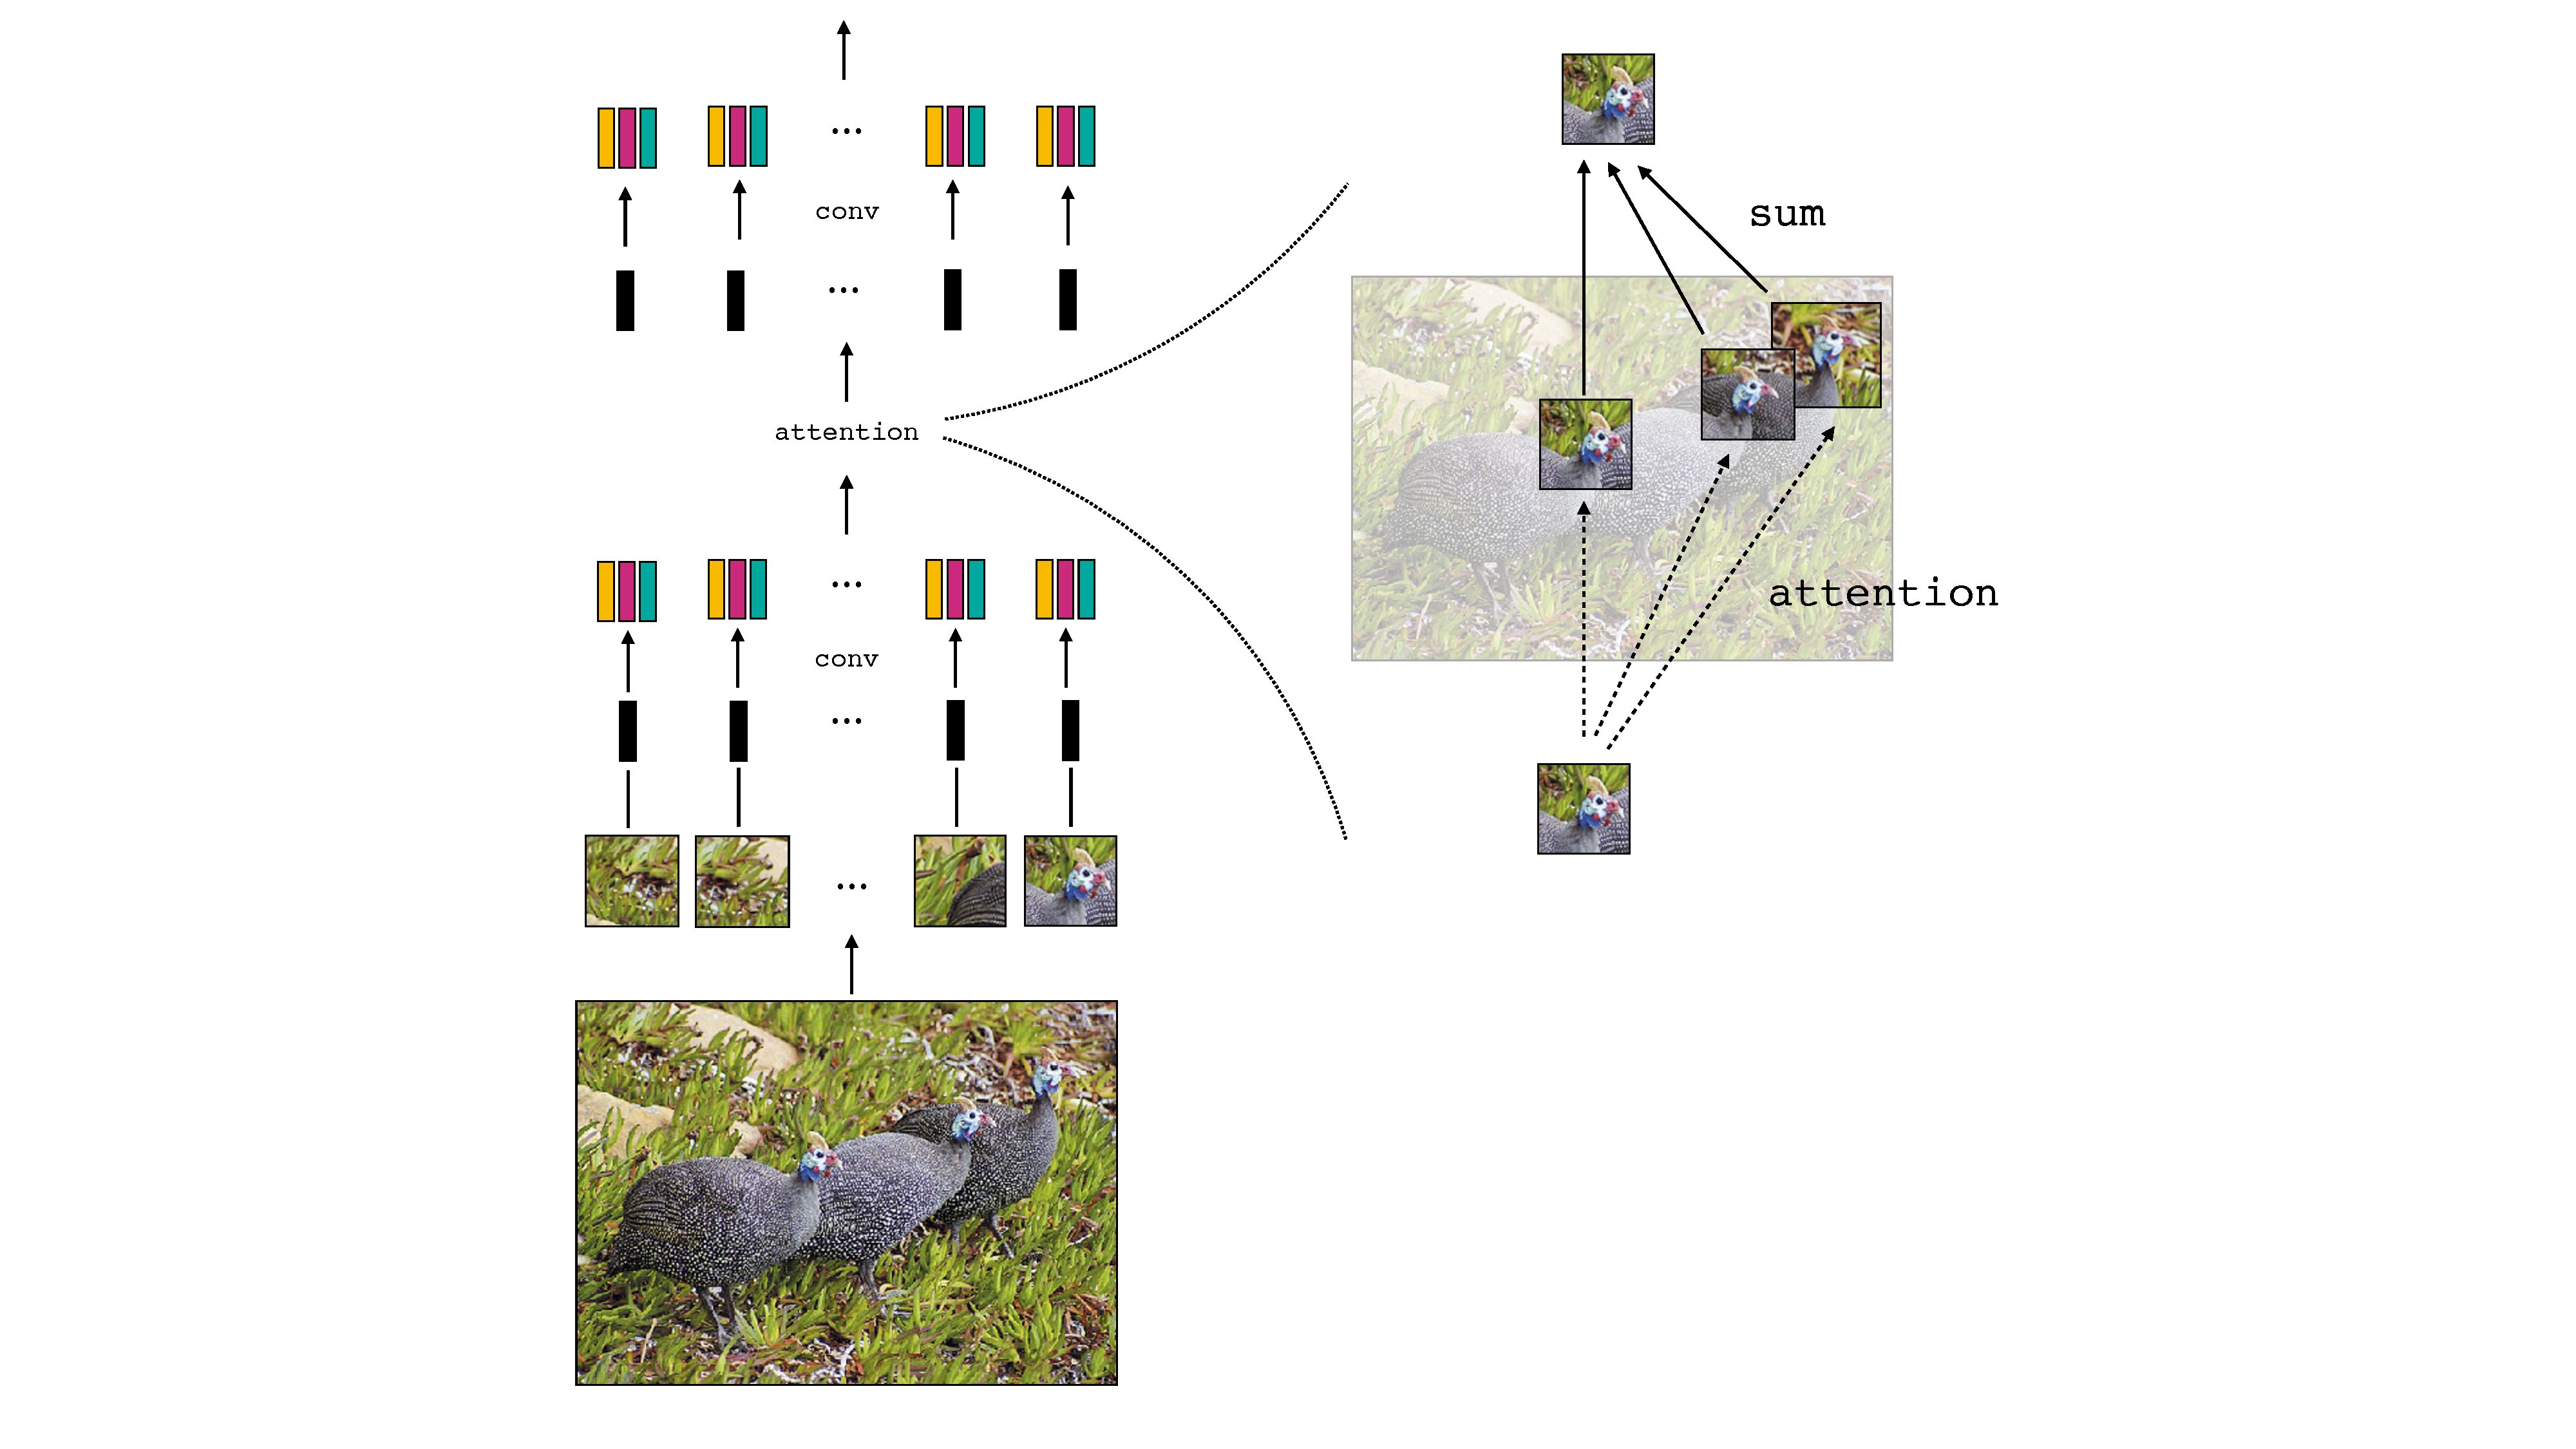
\includegraphics[width=0.8\linewidth]{./figures/transformers/transformer_arch.pdf}
%     }
%     \caption{Visualizing the full transformer architecture operating on an image.}
%     \label{fig:transformers:transformer_arch}
% \end{figure}

%Notice that most of the operations are familiar from the regular CNNs from Chapter \ref{chapter:convolutional_neural_nets}. As discussed in Section \ref{sec:transformers:modifying_tokens}, the per-token MLP layers are equivalent to CNNs with 1x1 spatial kernels. By a similar argument, it can be shown that the query, key, and value functions are equivalent to 1x1 convs over token code vectors (we leave this as an exercise to the reader). Normalization layers, softmax layers, and residual connections also appear in CNNs. The main novelty of transformers is the self-attention layer. These layers look like fully-connected layers but are importantly different in two ways:
%\begin{enumerate}
%    \item They operate over tokens rather than neurons.
%    \item The transformation parameters are a function of the input data.
%\end{enumerate}

%Therefore, we can see that transformers are intimately connected to both MLPs and CNNs, but differ from both in important ways.

\section{Permutation Equivariance}
An important property of transformers is that they are equivariant to permutations of the input token sequence. This follows from the fact that both tokenwise layers, $F_{\theta}$, and attention layers, $\texttt{attn}$, are \index{permutation equivariance}\textbf{permutation equivariant}:
\begin{align}
    F_{\theta}(\texttt{permute}(\tin))    & = \texttt{permute}(F_{\theta}(\tin))    \\
    \texttt{attn}(\texttt{permute}(\tin)) & = \texttt{permute}(\texttt{attn}(\tin))
\end{align}
where $\texttt{permute}$ is a permutation of the order of tokens in $\tin$ (i.e., permutes the rows of the matrix). This means that if you scramble (i.e. permute) the patches in the input image then apply attention, the output will be unchanged up to a permutation of the original output. Since the full transformer architecture is just composition of these two types of layers (plus, potentially, residual connections and token normalization, which are also permutation equivariant), and because composing two permutation equivariant functions results in a permutation equivariant operation, we have:
\begin{align}
    \texttt{transformer}(\texttt{permute}(\tin)) & = \texttt{permute}(\texttt{transformer}(\tin))
\end{align}
This property is visualized in \fig{\ref{fig:transformers:permutation_equivariance}}.

\begin{figure}[h]
    \centerline{
        \begin{minipage}{.32\linewidth}
            \begin{tikzpicture}
                %
                \def\Nnodes{3}
                \def\Nlayers{3}
                \def\layerheight{1.2}
                \def\neuronrad{0.3}
                \def\neuronstep{0.7}
                \def\tokennames {{"$\mathbf{t}_0$","$\mathbf{t}_1$","$\mathbf{t}_2$","$\mathbf{t}_3$"}}
                \foreach \x in {1,...,\Nnodes} {
                        \foreach \y in {1,...,\Nlayers} {
                                \draw (\neuronstep*\x-\neuronrad/4,\layerheight*\y-\layerheight-\neuronrad) rectangle ++(\neuronrad/2,\neuronrad*2);
                                \pgfmathparse{\tokennames[\x]};
                                \draw ($(\neuronstep*\x-\neuronrad,\layerheight*\y-\layerheight)$) node {\pgfmathresult};
                            }
                    }
                % mixing layer 1
                \foreach \xi in {1,...,\Nnodes} {
                        \foreach \xj in {1,...,\Nnodes} {
                                \draw [thick] [nn_edge] (\neuronstep*\xi,\neuronrad) -- (\neuronstep*\xj,\layerheight-\neuronrad);
                            }
                    }
                % pointwise nonlinearity
                \foreach \x in {1,...,\Nnodes} {
                        \draw [thick] [nn_edge] (\neuronstep*\x,\layerheight+\neuronrad) -- (\neuronstep*\x,\layerheight*2-\neuronrad);
                    }
                % arrow indicating permute
                \draw[->] (2.5,0) -- (5,0);
                \draw (7.5/2,0) node[fill=white] {\texttt{permute}};
            \end{tikzpicture}
        \end{minipage}
        \begin{minipage}{.19\linewidth}
            \begin{tikzpicture}
                %
                \def\Nnodes{3}
                \def\Nlayers{3}
                \def\layerheight{1.2}
                \def\neuronrad{0.3}
                \def\neuronstep{0.7}
                \def\tokennames {{"$\mathbf{t}_0$","$\mathbf{t}_2$","$\mathbf{t}_3$","$\mathbf{t}_1$"}}
                \foreach \x in {1,...,\Nnodes} {
                        \foreach \y in {1,...,\Nlayers} {
                                \draw (\neuronstep*\x-\neuronrad/4,\layerheight*\y-\layerheight-\neuronrad) rectangle ++(\neuronrad/2,\neuronrad*2);
                                \pgfmathparse{\tokennames[\x]};
                                \draw ($(\neuronstep*\x-\neuronrad,\layerheight*\y-\layerheight)$) node {\pgfmathresult};
                            }
                    }
                % mixing layer 1
                \foreach \xi in {1,...,\Nnodes} {
                        \foreach \xj in {1,...,\Nnodes} {
                                \draw [thick] [nn_edge] (\neuronstep*\xi,\neuronrad) -- (\neuronstep*\xj,\layerheight-\neuronrad);
                            }
                    }
                % pointwise nonlinearity
                \foreach \x in {1,...,\Nnodes} {
                        \draw [thick] [nn_edge] (\neuronstep*\x,\layerheight+\neuronrad) -- (\neuronstep*\x,\layerheight*2-\neuronrad);
                    }
            \end{tikzpicture}
        \end{minipage}
    }
    \caption{Transformers are permutation equivariant. For notational simplicity, we omit layer indices on the token variables here.}
    \label{fig:transformers:permutation_equivariance}
\end{figure}

It is often useful to understand layers in terms of their invariances and equivariances. Convolutational layers are translation equivariant but not necessarily permutation equivariant whereas attention layers are both translation equivariant \textit{and} permutation equivariant (since translation is a special kind of permutation, any permutation equivariant layer is also translation equivariant). %However, note that 1x1 convolutions are a special case of convolutions that are in fact permutation equivariant, because they are operate pointwise. 
Other layers can be catalogued similarly: global average pooling layers are permutation \textit{invariant}, relu layers are permutation equivariant, per-token MLP layers are also permutation equivariant (but with respect to sets of tokens rather than sets of neurons), and so on. %As we will see subsequently, all layers in standard transformers are permutation equivariant, so the entire transformer is permutation equivariant over its input tokens.

A generally good strategy is to select layers that reflect the symmetries in your data or task: in object detection, translation equivariance makes sense because, roughly, a bird is a bird no matter where it appears in an image. Permutation equivariance might also make sense, for that same reason, but only to an extent: if you break up an image into small patches and scramble them, this could disrupt spatial layout that is important for recognition. We will see in \sect{\ref{sec:transformers:positional_encodings}} how transformers use something called positional codes to reinsert useful information about spatial layout.

\section{CNNs in Disguise}

Transformers provide a new way of thinking about data processing, and it may seem like they are very different from past architectures. However, as we have alluded to, they actually have many commonalities with CNNs. In fact, most (but not all) of the transformer architecture can be viewed as a CNN in disguise. In this section we will walk through several of the layers we learned about above, and see how they are in fact performing convolutions.

\subsection{Tokenization}

The first step in working with transformers is to tokenize the input. The most basic way to do this is to chop up the input image into non-overlapping patches of size $K \times K$, then convert these patches to vectors via a linear projection. You might already have noticed that this operation can be written as convolution; after all we said the whole idea of CNNs is to chop the signal into patches. In particular, this form of tokenization can be written as a convolutional layer with kernel size and stride both equal to $K$:
\begin{align}
     & \mathbf{T}[n(N/K)+m,\cout] = \nonumber                                                                                                                                                                         \\
     & b[\cout] +  \sum_{\cin=1}^{\Cin} \sum_{k_1,k_2=-K}^K w[\cin,\cout,k_1,k_2] x_{\texttt{in}}[\cin,K n-k_1,K m-k_2] \quad \triangleleft \quad \text{(tokenization)} \label{eqn:transformers:tokenization_as_conv}
\end{align}
where, for RGB images, $\xin \in \mathbb{R}^{3 \times N \times M}$, $\Cin=3$, and $\Cout=d$ (the token dimensionality). This math assumes $N$ and $M$ are evenly divisible by $K$; if they aren't then the input can be resized or padded until they are.

Although the equation starts to look complicated, it is just a $\texttt{conv}$ operator with the following parameters:
\begin{minted}[xleftmargin=0.0\linewidth,xrightmargin=0.0\linewidth,
fontsize=\fontsize{8.5}{9},
frame=single,
framesep=2.5pt,
baselinestretch=1.05,
]{python}
T = conv(x_in, channels_in=3, channels_out=d, kernel=K, stride=K) # tokenize
\end{minted}

\subsection{Query-Key-Value Projections}

Next let's look at the query, key, and value projections that are part of the attention layers. For simplicity, we will consider just the query projection, since key and value follow exactly the same pattern.

We wrote this operation as a matrix multiply $\tin \mathbf{W}_q^\transpose$ (\eqn{\ref{eqn:transformers:query_matrix}}). What this multiply is doing is applying the same linear transformation ($\mathbf{W}_q$) to each token vector (each row of $\tin$). Applying the same linear operation to each element in a sequence is exactly what convolution does. Specifically, the query operation can be written as convolving the set of $N$ $d$-channel tokens with a filter bank of $m$ filters, with kernel size 1, producing a new set of $N$ $m$-channel tokens. This equivalence is visualized below (\fig{\ref{fig:transformers:conv_matmul_equivalence}}):
\begin{figure}[h!]
    \centerline{
        \begin{tikzpicture}
            % token sequence
            \def\Ntokens{4}
            \def\Nchannels{3}
            \def\Nfilters{4}
            \def\cellwidth{0.25}
            \def\neuronrad{0.3}

            %% draw conv
            % draw filter bank
            \foreach \x in {1,...,\Nfilters} {
                    \foreach \y in {1,...,\Nchannels} {
                            \draw [shift={(0, 0)}, fill=param_color, dotted] (\cellwidth*0.5*\x,-\cellwidth*\y-0.5*\cellwidth*\x) rectangle ++(\cellwidth,\cellwidth);
                        }
                    \draw [shift={(0, 0)}, thick] (\cellwidth*0.5*\x,-\cellwidth*\Nchannels-0.5*\cellwidth*\x) rectangle ++(\cellwidth,\cellwidth*\Nchannels);
                }
            \draw[decorate,decoration={brace, amplitude=5pt, angle=0}] (\cellwidth*3,-\cellwidth*\Nchannels*2+\cellwidth-0.1) -- (0,-\cellwidth*\Nchannels*2+\cellwidth-0.1);
            \node[below, rotate=0] at (\cellwidth*1.5,-\cellwidth*\Nchannels-\cellwidth*3.15) {$m$ filters};
            %
            \draw (\cellwidth*1.5,\cellwidth) node {$\mathbf{w}_q$};
            %
            \draw (1,-2.5*\cellwidth) node {$\star$};

            % draw signal
            % \foreach \y in {1,...,\Nchannels} {
            %     \foreach \x in {1,...,\Ntokens} {
            %         \draw [shift={(1, 0)}, fill=data_color] (\cellwidth*\x+0.5*\cellwidth*\y,-\cellwidth*\y*0.5) rectangle ++(\cellwidth,\cellwidth);
            %     }
            % }
            \foreach \x in {1,...,\Ntokens} {
                    \foreach \y in {1,...,\Nchannels} {
                            \draw [shift={(1, -\cellwidth)}, fill=data_color, dotted] (\cellwidth*\x,-\cellwidth*\y) rectangle ++(\cellwidth,\cellwidth);
                        }
                }
            \foreach \x in {1,...,\Ntokens} {
                    \draw [shift={(1, -\cellwidth)}, thick] (\cellwidth*\x,-\cellwidth*\Nchannels) rectangle ++(\cellwidth,\cellwidth*\Nchannels);
                }
            \draw[shift={(1.5, 0)}, decorate,decoration={brace, amplitude=5pt, angle=0}] (\cellwidth*3.25,-\cellwidth*\Nchannels*2+\cellwidth-0.1) -- (-0.25,-\cellwidth*\Nchannels*2+\cellwidth-0.1);
            \node[shift={(1.5, 0)}, below, rotate=0] at (\cellwidth*1.25,-\cellwidth*\Nchannels-\cellwidth*3.15) {$N$ tokens};
            %
            \draw[shift={(1.5, 0)}, decorate,decoration={brace, amplitude=5pt, angle=0}] (\cellwidth*3.5,-\cellwidth) -- (\cellwidth*3.5,-\cellwidth*4);
            \node[shift={(1.5, 0)}, right, rotate=90] at (\cellwidth*5,-\cellwidth*\Nchannels-\cellwidth*3.15) {$d$ channels};
            %
            \draw[shift={(1.5, 0)}] (\cellwidth*1.25,\cellwidth) node {$\tin^\transpose$};

            %
            \draw (4, -2.5*\cellwidth) node {$\Longleftrightarrow$};

            %% draw matmul
            % draw T
            %\def\colors{{"red", "green", "blue"}}
            \foreach \x in {1,...,\Nchannels} {
                    \foreach \y in {1,...,\Ntokens} {
                            %\pgfmathparse{\colors[\x-1]}
                            %\edef\colorvalue{\pgfmathresult}
                            %\draw [shift={(4, 0)}, fill=\colorvalue] (\cellwidth*\x,-\cellwidth*\y) rectangle ++(\cellwidth,\cellwidth);
                            \draw [shift={(5, 0)}, fill=data_color, dotted] (\cellwidth*\x,-\cellwidth*\y-0.5*\cellwidth) rectangle ++(\cellwidth,\cellwidth);
                        }
                }
            \foreach \y in {1,...,\Ntokens} {
                    \draw [shift={(5, 0)}, thick] (\cellwidth,-\cellwidth*\y-0.5*\cellwidth) rectangle ++(\cellwidth*\Nchannels,\cellwidth);
                }
            \draw[shift={(5, 0)}] (\cellwidth*2.5,\cellwidth) node {$\tin$};
            %
            % draw W^T
            \foreach \x in {1,...,\Nfilters} {
                    \foreach \y in {1,...,\Nchannels} {
                            \draw [shift={(5, 0)}, fill=param_color, dotted] (3.5*\cellwidth+\cellwidth*\x,-\cellwidth*\y-0.5*\cellwidth) rectangle ++(\cellwidth,\cellwidth);
                        }
                }
            \foreach \x in {1,...,\Nfilters} {
                    \draw [shift={(5, 0)}, thick] (3.5*\cellwidth+\cellwidth*\x,-\cellwidth*\Nchannels-0.5*\cellwidth) rectangle ++(\cellwidth,\cellwidth*\Nchannels);
                }
            \draw[shift={(5, 0)}] (\cellwidth*6.5,\cellwidth) node {$\mathbf{W}_q^\transpose$};
            %
            \draw[shift={(0, 0)}] (\cellwidth*5.25,1) node {\underline{Convolution with filters of kernel size 1}};
            \draw[shift={(5, 0)}] (\cellwidth*4.5,1) node {\underline{Matrix multiply}};
        \end{tikzpicture}
    }
    \caption{The query, key, and value projections in transformers can be written either as a convolution or a matrix multiply.}
    \label{fig:transformers:conv_matmul_equivalence}
\end{figure}

Therefore, the query, key, and value projections are all multichannel convolutions with kernels of size 1.\marginnote{Convolution actually appears all over in linear algebra, and in fact \textit{every matrix product can be written as a convolution}! Whenever you see a product $\mathbf{A}\mathbf{B}$, you can think of it as the convolution of a multichannel filter bank $\mathbf{B}$ (one filter in each row; kernel size 1) with the signal $\mathbf{A}$ (time indexes rows, channels in the columns).}[-2.0cm]

% Notice that once again we have an operation, here, that applies the same transformation independently and identically to all tokens in the input set. You should recognize that this again is a convolution; the query/key/value transformations can be written as a bank of $m$ linear filters, each of which operates over a 1D signal with $d$ channels -- the sequence of tokens.\marginnote{Convolution actually appears all over in linear algebra, and in fact \textit{every matrix product can be written as a convolution}! Whenever you see a product $\mathbf{A}\mathbf{B}$, you can think of it as the convolution of a multichannel filter bank $\mathbf{B}$ (one filter in each row; kernel size 1) with the signal $\mathbf{A}$ (time indexes rows, channels in the columns).}% The converse is also true: every convolution can be written as a matrix product. This is because any linear operator can be written as a matrix, and convolutions are linear operators.}
% \begin{align}
%     \Qin = \mathbf{w}_q \star \tin^\transpose
% \end{align}
% where $\mathbf{w}_q \in \mathbb{R}^{1 \times m \times d}$ is a filter bank with $m$ filters operating over $d$ channels, with weights $\mathbf{w}_q[0,:,:,] = \mathbf{W}_q$. The same can be written for $\Kin$ and $\Vin$.


\subsection{Tokenwise MLP}
%[Just say it's the same as query-key-value projections. First show that the linear layers in MLP are per-token projection and can be written as $\tin \mathbf{W}^\transpose$. Then these are equiv to conv by previous section. And relu is unchanged. So token-wise MLP is just convs and relus hence a CNN.]

%Next we will consider the token-wise MLP layer. We will show that this is equivalent to 1x1 convolutions interleaved with neuron-wise nonlinearities, i.e. it's a CNN. %, which play the role of the pointwise nonlinearities in transformers. We will show that a token-wise MLP is in fact equivalent to a CNN, again with 1x1 kernels, applied to the token sequence. The argument here is very similar as for the query-key-value projections.

Next we will consider the token-wise MLP layer. A token-wise MLP applies the same MLP $F_{\theta}$ to each token in a sequence. The $F_{\theta}$ consists of linear layers and pointwise nonlinearities. For simplicity, we will assume no biases (as an exercise, this can be relaxed). The linear layers in $F_{\theta}$ all have the following form:
\begin{align}
    \mathbf{t}_{\texttt{out}} & = \mathbf{W}\mathbf{t}_{\texttt{in}}
\end{align}
When we apply such a layer to each token in the sequence, we have:
\begin{align}
    \tout & = \tin\mathbf{W}^{\transpose}
\end{align}
Notice that this looks just like the query operation we covered in the previous section, \eqn{\ref{eqn:transformers:query_matrix}}. Therefore, the same result holds: the linear layers of the token-wise MLP can all be written as convolutions with kernel size 1.
%\marginnote{We use the term ``1x1 filter'' to refer to any filter whose kernel size is 1 in all its dimensions, regardless of whether the signal is 1D, 2D, 3D, etc.}[-2cm]

Now the pointwise nonlinearities in the MLP are applied neuronwise, so these layers function identically to the pointwise nonlinearity in CNNs. This is the full set of layers in the MLP, and therefore we have that a token-wise MLP can be written as a series of convolutions interleaved with neuronwise-nonlinearities, i.e. a CNN.

% Consider an MLP with one hidden layer and two linear layers: \texttt{linear}-\texttt{relu}-\texttt{linear}. To create our token-wise MLP layer, we will apply this MLP to each token in a sequence. The MLP takes a vector $\mathbf{t}$ as input and is defined as follows:
% \begin{align}
%     \mathbf{a} &= \mathbf{W}_1\mathbf{t} + \mathbf{b}_1 &\quad\quad \triangleleft \quad \texttt{linear}\\
%     \mathbf{h} &= \texttt{relu}(\mathbf{a}) &\quad\quad \triangleleft \quad \texttt{relu}\\
%     \mathbf{z} &= \mathbf{W}_2\mathbf{h} + \mathbf{b}_2 &\quad\quad \triangleleft \quad \texttt{linear}
% \end{align}
% Notice that each linear layer has the same form as a query/key/value projection: the same linear operation applied to each token (except with a bias this time). We already saw that this can be written as a convolution in the last section, so we have:
% \begin{align}
%     \mathbf{A} &= \tin\mathbf{W}_1^{\tranpose} + \mathbf{B}_1 &\quad\quad \triangleleft \quad \texttt{linear}
% \end{align}

% Then the per-token nonlinearity layer over an input sequence $\tin[0,:], \ldots, \tin[N-1,:]$ is:
% \begin{align}
%     \tout = \begin{bmatrix}
%         \texttt{MLP}(\tin[0,:])^\transpose\\
%         \vdots\\
%         \texttt{MLP}(\tin[N,:])^\transpose
%     \end{bmatrix}
% \end{align}


% Now consider a CNN with one hidden layer and two convolutional layers: \texttt{conv}-\texttt{relu}-\texttt{conv}, defined as follows:
% \begin{align}
%     \mathbf{a} &= \mathbf{w}_1 \star \tin + \mathbf{b}_1 &\quad\quad \triangleleft \quad \texttt{conv}\\
%     \mathbf{h} &= \texttt{relu}(\mathbf{a}) &\quad\quad \triangleleft \quad \texttt{relu}\\
%     \tout &= \mathbf{w}_2 \star \mathbf{h} + \mathbf{b}_2 &\quad\quad \triangleleft \quad \texttt{conv}
% \end{align}\marginnote{Remember, we use lowercase for tensors in CNNs and stick with that convention here. $\mathbf{a}$ is a tensor of shape $[N \times \Cout]$. Also, note that we use $\texttt{relu}(\mathbf{x})$ to me applying the $\texttt{relu}$ function to each scalar element of the tensor $\mathbf{x}$.}}[-0.4cm]
% We can rewrite any 1x1 conv layer with filter $\mathbf{w} \in \mathbb{R}^{\Cin \times \Cout \times 1 \times 1}$ as:
% \begin{align}
%     \mathbf{a} &= \begin{bmatrix}
%         (\mathbf{w}[:,:,0,0]^\transpose \tin[0,:] + \mathbf{b})^\transpose\\
%         \vdots\\
%         (\mathbf{w}[:,:,0,0]^\transpose \tin[N-1,:] + \mathbf{b})^\transpose
%     \end{bmatrix}
% \end{align}
% Now if we use the same weights as in the MLP (specifically, $\mathbf{w}_1[:,:,0,0]^\transpose = \mathbf{W}_1$ and $\mathbf{w}_2[:,:,0,0]^\transpose = \mathbf{W}_2e$), then we have the CNN performing:
% \begin{align}
%     \mathbf{a} &= \begin{bmatrix}
%         (\mathbf{W}_1\tin[0,:] + \mathbf{b}_1)^\transpose\\
%         \vdots\\
%         (\mathbf{W}_1\tin[N-1,:] + \mathbf{b}_1)^\transpose
%     \end{bmatrix}\\
%     \mathbf{h} &= \begin{bmatrix}
%         \texttt{relu}(\mathbf{a}[0,:])\\
%         \vdots\\
%         \texttt{relu}(\mathbf{a}[N-1,:])
%     \end{bmatrix}\\
%     \tout &= \begin{bmatrix}
%         (\mathbf{W}_2\mathbf{h}[0,:] + \mathbf{b}_1)^\transpose\\
%         \vdots\\
%         (\mathbf{W}_2\mathbf{h}[N-1,:] + \mathbf{b}_1)^\transpose
%     \end{bmatrix}
% \end{align}
% Now we have rewritten the CNN as a per-token MLP, showing that:
% \begin{align}
%     \tout &= \texttt{CNN}(\tin)\\
%           &= \begin{bmatrix}
%               \texttt{MLP}(\tin[0,:])^\transpose\\
%               \vdots\\
%               \texttt{MLP}(\tin[N-1,:])^\transpose
%           \end{bmatrix}
% \end{align}
%\marginnote{With kernel size 1, there is no spatial overlap between adjacent applications of the filter. This means that it doesn't actually matter which indices are next to which. You can permute the indices of the input and the only thing that changes is the indices of the output will be permuted in the same order. This makes filters of kernel size 1 not just translation equivariant (like all filters) but in fact also \textit{permutation equivariant} (a stronger symmetry). We will come back to this idea at the end of this chapter.}

\subsection{The Similarities between CNNs and Transfomers}
As we have now seen, most layers in transformers are convolutional. These layers break up the signal processing problem into chunks, then process each chunk independently and identically.\marginnote{Breaking up into chunks is such a fundamentally useful idea that it shows up in many different fields under different names. One general name for it is \textbf{factorizing} a problem into smaller pieces.}[-1.6cm] Some of the other operations in transformers -- normalization layers, residual connections, etc -- are also common in CNNs. So what is \textit{different} between transformers and CNNs?

\subsection{The Differences between CNNs and Transformers}

\subsubsection{CNNs can have kernels with non-unitary spatial extent}
When we wrote them as convolutions, the query-key-value projections and token-wise MLPs \textit{only used 1x1 filters}.\marginnote{We use the term ``1x1 filter'' to refer to any filter whose kernel size is 1 in all its dimensions, regardless of whether the signal is one-dimensional, two-dimensional, three-dimensional, etc.}[-0.4cm] In fact it cannot be otherwise. If you used larger kernel it would break the permutation invariance property of transformers, since the output of the filters would depend on which token is next to which. This is one of the key differences between CNNs and transformers. CNNs use $K \times K$ filters, and this makes it so adjacent image regions get processed together. Transformers use 1x1 filters which means the network has no architectural way of knowing about spatial structure (which token is next to which). For vision problems, where spatial structure is often crucially important, transformers can instead be given knowledge of position through the \textit{inputs} to the network, rather than through the architectural structure. We will cover this idea in \sect{\ref{sec:transformers:positional_encodings}}.

\subsubsection{Transformers have attention layers}
Attention layers are \textit{not} convolutional. They do not factor the processing into independent chunks but instead perform a global operation, in which all input tokens can interact. The linear combination of tokens that results is not a mixing operation found in CNNs and addresses the limitation of CNNs being myopic, with each filter only seeing information in its receptive field.


\section{Masked Attention}\label{sec:transformers:masked_attention}
\index{Attention!Masked attention}
Sometimes we want to restrict which tokens can attend to which. This can be done by \textit{masking} the attention matrix, which just means fixing some of the weights to be zero. This can be useful for many settings, including learning features via masked autoencoding~\cite{he2022masked}, cross-attention between different data modalities~\cite{wei2020multi}, and for sequential prediction~\cite{chen2020generative}. To illustrate, we will describe the sequential prediction use case.
\marginnote{For simplicity, in this section we depict tokens with one-dimensional code vectors, but remember $\mathbf{T}$ would have $d$ columns for $d$-dimensional code vectors.}[-2cm]

A common problem is to predict the $(n+1)$-th token in a sequence given the previous $n$ tokens. For example, we may be trying to predict tokens that represent the next frame in a video, the next word in a sentence, or the weather on the next day.

A simple way to model this prediction problem is with a linear layer: $\mathbf{y}_{n+1} = \mathbf{A}\mathbf{T}_{1:n}$.\marginnote{The $\mathbf{T}_{1:n}$ is shorthand for the sequence of tokens $\begin{bmatrix}
            \mathbf{t}_1^\transpose \\
            \vdots                  \\
            \mathbf{t}_{n}^\transpose
        \end{bmatrix}$.}[-0.6cm]
Here is what this looks like diagrammatically, and on the right is the layer shown as matrix multiplication:
%\newgeometry{papersize={8in,9in},bottom=3pc,top=5pc,left=6pc,right=12pc,headsep=2pc,marginparwidth=8pc, marginparsep=1pc, textwidth=30pc, textheight=45pc}
\begin{figure}[h]
    \centerline{
        \begin{minipage}{.49\linewidth}
            \centering
            \begin{tikzpicture}
                %
                \def\Nnodes{3}
                \def\Nnodesplusone{4}
                \def\layerheight{1.6}
                \def\neuronrad{0.3}
                \def\neuronstep{0.7}
                % time bars
                \foreach \x in {1,...,\Nnodesplusone} {
                        \draw [dotted, thick] (\neuronstep*\x,-\layerheight*0.5) -- (\neuronstep*\x,\layerheight*1.3);
                    }
                % input sequence
                \foreach \x in {1,...,\Nnodes} {
                        \draw [fill=white] (\neuronstep*\x-\neuronrad/4,-\neuronrad) rectangle ++(\neuronrad/2,\neuronrad*2);
                    }
                % output target
                \draw [fill=white] (\neuronstep*\Nnodes+\neuronstep-\neuronrad/4,\layerheight-\neuronrad) rectangle ++(\neuronrad/2,\neuronrad*2);
                %\draw (\neuronstep*\Nnodes+\neuronstep,\layerheight+\neuronrad*2) node {$t_{n+1}$};
                % linear layer
                \foreach \xi in {1,...,\Nnodes} {
                        \draw [thick] [nn_edge] ($(\neuronstep*\xi,\neuronrad)$) -- ($(\neuronstep*\Nnodes+\neuronstep,\layerheight-\neuronrad)$);
                    }
                % time steps
                \def\tokennames {{"$0$","$1$","$2$","$3$","$4$"}}
                \foreach \xi in {1,...,\Nnodesplusone} {
                        \pgfmathparse{\tokennames[\xi]};
                        \draw ($(\neuronstep*\xi,-\neuronrad*2.4)$) node [fill=white] {\pgfmathresult};
                    }
                \draw ($(-\neuronstep,-\neuronrad*2.4)$) node {time index:};
                %
                \draw (2.2,0.5*\layerheight) node[draw,rectangle,fill=white] {$\mathbf{A}$};
                %
            \end{tikzpicture}
        \end{minipage}
        \begin{minipage}{.49\linewidth}
            \centering
            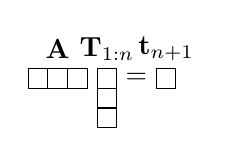
\begin{tikzpicture}
                % W matrix
                \def\Nx{3}
                \def\Ny{1}
                \def\cellwidth{0.25}
                \foreach \x in {1,...,\Nx} {
                        \foreach \y in {1,...,\Ny} {
                                \draw [fill=white] (\cellwidth*\x-\cellwidth,\cellwidth*\y-\cellwidth) rectangle ++(\cellwidth,\cellwidth);
                            }
                    }
                \draw (\cellwidth*\Nx*0.5, \cellwidth*2) node {$\mathbf{A}$};
                % token sequence
                \def\Nx{1}
                \def\Ny{3}
                \def\cellwidth{0.25}
                \foreach \x in {1,...,\Nx} {
                        \foreach \y in {1,...,\Ny} {
                                \draw [fill=white] (\cellwidth*\x+\cellwidth*3.5-\cellwidth,-\cellwidth*\y+\cellwidth) rectangle ++(\cellwidth,\cellwidth);
                            }
                    }
                \draw (\cellwidth*0.5+\cellwidth*3.5, \cellwidth*2) node {$\mathbf{T}_{1:n}$};
                %
                \draw (\cellwidth*0.5+\cellwidth*5, \cellwidth/2) node {$=$};
                % token output
                \draw [fill=white] (\cellwidth+\cellwidth*6.5-\cellwidth,\cellwidth-\cellwidth) rectangle ++(\cellwidth,\cellwidth);
                \draw (\cellwidth*0.5+\cellwidth*6.5, \cellwidth*2) node {$\mathbf{t}_{n+1}$};
            \end{tikzpicture}
        \end{minipage}
    }
    \caption{Masked prediction of time index 4 from time indices 1-3.}
\end{figure}

During training, we will give examples like this:
\begin{align}
    \{\mathbf{t}_1, \ldots, \mathbf{t}_n\}     & \rightarrow \mathbf{t}_{n+1} \label{eqn:transformers:causal_training_batches} \\
    \{\mathbf{t}_1, \ldots, \mathbf{t}_{n-1}\} & \rightarrow \mathbf{t}_n                                                      \\
    \{\mathbf{t}_1, \ldots, \mathbf{t}_{n-2}\} & \rightarrow \mathbf{t}_{n-1}
\end{align}
and so on. We can make all these predictions at once with a single matrix multiply (\fig{\ref{fig:transformers:masked_attn_one_matmul}}):
\begin{figure}[h]
    \centerline{
        \begin{minipage}{.49\linewidth}
            \centering
            \begin{tikzpicture}
                %
                \def\Nnodes{3}
                \def\Nnodesplusone{4}
                \def\layerheight{1.6}
                \def\neuronrad{0.3}
                \def\neuronstep{0.7}
                % time bars
                \foreach \x in {1,...,\Nnodesplusone} {
                        \draw [dotted, thick] (\neuronstep*\x,-\layerheight*0.5) -- (\neuronstep*\x,\layerheight*1.3);
                    }
                % input sequence
                \foreach \x in {1,...,\Nnodes} {
                        \draw [fill=white] (\neuronstep*\x-\neuronrad/4,-\neuronrad) rectangle ++(\neuronrad/2,\neuronrad*2);
                    }
                % output target
                \foreach \x in {2,...,\Nnodesplusone} {
                        \draw [fill=white] (\neuronstep*\x-\neuronrad/4,\layerheight-\neuronrad) rectangle ++(\neuronrad/2,\neuronrad*2);
                    }
                %\draw (\neuronstep*\Nnodes+\neuronstep,\layerheight+\neuronrad*2) node {$t_{n+1}$};
                % linear layer
                \foreach \xi in {1,...,\Nnodes} {
                        \foreach \yi in {2,...,\Nnodesplusone} {
                                \ifthenelse{\yi>\xi}{
                                    \draw [thick] [nn_edge] ($(\neuronstep*\xi,\neuronrad)$) -- ($(\neuronstep*\yi,\layerheight-\neuronrad)$);
                                }{}
                            }
                    }
                % time steps
                \def\tokennames {{"$0$","$1$","$2$","$3$","$4$"}}
                \foreach \xi in {1,...,\Nnodesplusone} {
                        \pgfmathparse{\tokennames[\xi]};
                        \draw ($(\neuronstep*\xi,-\neuronrad*2.4)$) node [fill=white] {\pgfmathresult};
                    }
                \draw ($(-\neuronstep,-\neuronrad*2.4)$) node {time index:};
                %
                \draw (2.5*\neuronstep,0.5*\layerheight) node[draw,rectangle,fill=white] {$\mathbf{A}$};
                %
            \end{tikzpicture}
            \centering
        \end{minipage}
        \begin{minipage}{.49\linewidth}
            \centering
            \begin{tikzpicture}
                % W matrix
                \def\Nx{4}
                \def\Ny{4}
                \def\cellwidth{0.25}
                \foreach \x in {1,...,\Nx} {
                        \foreach \y in {1,...,\Ny} {
                                \def\xplusone{\x+1};
                                \ifthenelse{\y>\xplusone}{\definecolor{cellfill}{rgb}{1,1,1}}{\definecolor{cellfill}{rgb}{0,0,0}};
                                \draw [fill=cellfill] (\cellwidth*\x-\cellwidth,-\cellwidth*\y+\cellwidth) rectangle ++(\cellwidth,\cellwidth);
                            }
                    }
                \draw (\cellwidth*\Nx*0.5, \cellwidth*2) node {$\mathbf{A}$};
                % token sequence
                \def\Nx{1}
                \def\Ny{4}
                \def\cellwidth{0.25}
                \foreach \x in {1,...,\Nx} {
                        \foreach \y in {1,...,\Ny} {
                                \draw [fill=white] (\cellwidth*\x+\cellwidth*4.5-\cellwidth,-\cellwidth*\y+\cellwidth) rectangle ++(\cellwidth,\cellwidth);
                            }
                    }
                \draw [fill=black] (\cellwidth+\cellwidth*4.5-\cellwidth,-\cellwidth*4+\cellwidth) rectangle ++(\cellwidth,\cellwidth);
                \draw (\cellwidth*0.5+\cellwidth*4.5, \cellwidth*2) node {$\tin$};
                %
                \draw (\cellwidth*0.5+\cellwidth*6, \cellwidth/2) node {$=$};
                % token output
                \def\Nx{1}
                \def\Ny{4}
                \def\cellwidth{0.25}
                \foreach \x in {1,...,\Nx} {
                        \foreach \y in {1,...,\Ny} {
                                \draw [fill=white] (\cellwidth*\x+\cellwidth*7.5-\cellwidth,-\cellwidth*\y+\cellwidth) rectangle ++(\cellwidth,\cellwidth);
                            }
                    }
                \draw [fill=black] (\cellwidth+\cellwidth*7.5-\cellwidth,-\cellwidth*1+\cellwidth) rectangle ++(\cellwidth,\cellwidth);
                \draw (\cellwidth*0.5+\cellwidth*7.5, \cellwidth*2) node {$\tout$};
            \end{tikzpicture}
        \end{minipage}
    }
    \caption{Masked attention to make multiple causal predictions at once. Black cells are masked; they are filled with zeros.}
    \label{fig:transformers:masked_attn_one_matmul}
\end{figure}

This way, one forward pass makes $N$ predictions rather than one prediction. This is equivalent to doing a single next token prediction $N$ times, but it all happens in a single matrix multiply, using the matrix shown on the right.

This kind of matrix is called \textit{causal} because each output index $i$ only depends on input indices $j$ such that $j < i$. If $\mathbf{A}$ is an attention matrix, then this strategy is called \index{Attention!Causal attention}\textbf{causal attention}. This is a masking strategy where each token can only attend to \textit{previous} tokens in the sequence. This approach can dramatically speed up training because all the sub-sequence prediction problems (predict $\mathbf{t}_{n-1}$ given $\mathbf{T}_{1:n-2}$, predict $\mathbf{t}_{n}$ given $\mathbf{T}_{1:n-1}$, predict $\mathbf{t}_{n+1}$ given $\mathbf{T}_{1:n}$) are supervised at the same time.

This also works for transformers with more than one layer, where the masking strategy looks like shown in \fig{\ref{fig:transformers:multilayer_masked_attention}}.
\begin{figure}[h]
    \centerline{
        \begin{minipage}{.49\linewidth}
            \centering
            \begin{tikzpicture}
                %
                \def\Nnodes{3}
                \def\Nnodesplusone{4}
                \def\layerheight{1.6}
                \def\neuronrad{0.3}
                \def\neuronstep{0.7}
                % time bars
                \foreach \x in {1,...,\Nnodesplusone} {
                        \draw [dotted, thick] (\neuronstep*\x,-\layerheight*0.5) -- (\neuronstep*\x,\layerheight*3.3);
                    }
                % input sequence
                \foreach \x in {1,...,\Nnodes} {
                        \draw [fill=white] (\neuronstep*\x-\neuronrad/4,-\neuronrad) rectangle ++(\neuronrad/2,\neuronrad*2);
                    }
                % hidden layer 1
                \foreach \x in {2,...,\Nnodesplusone} {
                        \draw [fill=white] (\neuronstep*\x-\neuronrad/4,\layerheight-\neuronrad) rectangle ++(\neuronrad/2,\neuronrad*2);
                    }
                %\draw (\neuronstep*\Nnodes+\neuronstep,\layerheight+\neuronrad*2) node {$t_{n+1}$};
                % linear layer
                \foreach \xi in {1,...,\Nnodes} {
                        \foreach \yi in {2,...,\Nnodesplusone} {
                                \ifthenelse{\yi>\xi}{
                                    \draw [thick] [nn_edge] ($(\neuronstep*\xi,\neuronrad)$) -- ($(\neuronstep*\yi,\layerheight-\neuronrad)$);
                                }{}
                            }
                    }
                % pointwise nonlinearity
                \foreach \x in {2,...,\Nnodesplusone} {
                        \draw [thick] [nn_edge] (\neuronstep*\x,\layerheight+\neuronrad) -- (\neuronstep*\x,\layerheight*2-\neuronrad);
                    }
                % hidden layer 2
                \foreach \x in {2,...,\Nnodesplusone} {
                        \draw [fill=white] (\neuronstep*\x-\neuronrad/4,\layerheight*2-\neuronrad) rectangle ++(\neuronrad/2,\neuronrad*2);
                    }
                % linear layer
                \foreach \xi in {2,...,\Nnodesplusone} {
                        \foreach \yi in {2,...,\Nnodesplusone} {
                                \pgfmathparse{\xi-1}
                                \ifthenelse{\yi>\pgfmathresult}{
                                    \draw [thick] [nn_edge] ($(\neuronstep*\xi,2*\layerheight+\neuronrad)$) -- ($(\neuronstep*\yi,3*\layerheight-\neuronrad)$);
                                }{}
                            }
                    }
                % output layer
                \foreach \x in {2,...,\Nnodesplusone} {
                        \draw [fill=white] (\neuronstep*\x-\neuronrad/4,\layerheight*3-\neuronrad) rectangle ++(\neuronrad/2,\neuronrad*2);
                    }
                % time steps
                \def\tokennames {{"$0$","$1$","$2$","$3$","$4$"}}
                \foreach \xi in {1,...,\Nnodesplusone} {
                        \pgfmathparse{\tokennames[\xi]};
                        \draw ($(\neuronstep*\xi,-\neuronrad*2.4)$) node [fill=white] {\pgfmathresult};
                    }
                \draw ($(-\neuronstep,-\neuronrad*2.4)$) node {time index:};
                %
                \draw (2.5*\neuronstep,0.5*\layerheight) node[draw,rectangle,fill=white] {$\mathbf{A}_1$};
                \draw (3*\neuronstep,2.5*\layerheight) node[draw,rectangle,fill=white] {$\mathbf{A}_2$};
                %
            \end{tikzpicture}
        \end{minipage}
        \begin{minipage}{.49\linewidth}
            \centering
            \begin{tikzpicture}
                \def\layerheight{1.6}
                % W matrix
                \def\Nx{3}
                \def\Ny{3}
                \def\cellwidth{0.25}
                \foreach \x in {1,...,\Nx} {
                        \foreach \y in {1,...,\Ny} {
                                \ifthenelse{\y<\x}{\definecolor{cellfill}{rgb}{0,0,0}}{\definecolor{cellfill}{rgb}{1,1,1}};
                                \draw [fill=cellfill] (\cellwidth*\x-\cellwidth,-\cellwidth*\y+2.5*\layerheight) rectangle ++(\cellwidth,\cellwidth);
                            }
                    }
                \draw (\cellwidth*\Nx*0.5, \cellwidth+2.5*\layerheight) node {$\mathbf{A}_2$};
                % token sequence
                \def\Nx{1}
                \def\Ny{3}
                \def\cellwidth{0.25}
                \foreach \x in {1,...,\Nx} {
                        \foreach \y in {1,...,\Ny} {
                                \draw [fill=white] (\cellwidth*\x+\cellwidth*4.5-\cellwidth,-\cellwidth*\y+2.5*\layerheight) rectangle ++(\cellwidth,\cellwidth);
                            }
                    }
                \draw (\cellwidth*0.5+\cellwidth*4.5, \cellwidth+2.5*\layerheight) node {$\tin$};
                %
                \draw (\cellwidth*0.5+\cellwidth*6, -\cellwidth/2+2.5*\layerheight) node {$=$};
                % token output
                \def\Nx{1}
                \def\Ny{3}
                \def\cellwidth{0.25}
                \foreach \x in {1,...,\Nx} {
                        \foreach \y in {1,...,\Ny} {
                                \draw [fill=white] (\cellwidth*\x+\cellwidth*7.5-\cellwidth,-\cellwidth*\y+2.5*\layerheight) rectangle ++(\cellwidth,\cellwidth);
                            }
                    }
                \draw (\cellwidth*0.5+\cellwidth*7.5, \cellwidth+2.5*\layerheight) node {$\tout$};
                %
                % W matrix
                \def\Nx{4}
                \def\Ny{4}
                \def\cellwidth{0.25}
                \foreach \x in {1,...,\Nx} {
                        \foreach \y in {1,...,\Ny} {
                                \def\xplusone{\x+1};
                                \ifthenelse{\y>\xplusone}{\definecolor{cellfill}{rgb}{1,1,1}}{\definecolor{cellfill}{rgb}{0,0,0}};
                                \draw [fill=cellfill] (\cellwidth*\x-\cellwidth,-\cellwidth*\y+\cellwidth) rectangle ++(\cellwidth,\cellwidth);
                            }
                    }
                \draw (\cellwidth*\Nx*0.5, \cellwidth*2) node {$\mathbf{A}_1$};
                % token sequence
                \def\Nx{1}
                \def\Ny{4}
                \def\cellwidth{0.25}
                \foreach \x in {1,...,\Nx} {
                        \foreach \y in {1,...,\Ny} {
                                \draw [fill=white] (\cellwidth*\x+\cellwidth*4.5-\cellwidth,-\cellwidth*\y+\cellwidth) rectangle ++(\cellwidth,\cellwidth);
                            }
                    }
                \draw [fill=black] (\cellwidth+\cellwidth*4.5-\cellwidth,-\cellwidth*4+\cellwidth) rectangle ++(\cellwidth,\cellwidth);
                \draw (\cellwidth*0.5+\cellwidth*4.5, \cellwidth*2) node {$\tin$};
                %
                \draw (\cellwidth*0.5+\cellwidth*6, \cellwidth/2) node {$=$};
                % token output
                \def\Nx{1}
                \def\Ny{4}
                \def\cellwidth{0.25}
                \foreach \x in {1,...,\Nx} {
                        \foreach \y in {1,...,\Ny} {
                                \draw [fill=white] (\cellwidth*\x+\cellwidth*7.5-\cellwidth,-\cellwidth*\y+\cellwidth) rectangle ++(\cellwidth,\cellwidth);
                            }
                    }
                \draw [fill=black] (\cellwidth+\cellwidth*7.5-\cellwidth,-\cellwidth*1+\cellwidth) rectangle ++(\cellwidth,\cellwidth);
                \draw (\cellwidth*0.5+\cellwidth*7.5, \cellwidth*2) node {$\tout$};
                %
                % W matrix
                % \def\Nx{3}
                % \def\Ny{3}
                % \def\cellwidth{0.25}
                % \foreach \x in {1,...,\Nx} {
                %     \foreach \y in {1,...,\Ny} {
                %         \ifthenelse{\y>\x}{\definecolor{cellfill}{rgb}{1,1,1}}{\definecolor{cellfill}{rgb}{0,0,0}};
                %         \draw [fill=cellfill] (\cellwidth*\x-\cellwidth,-\cellwidth*\y+\cellwidth+0.5*\layerheight) rectangle ++(\cellwidth,\cellwidth);
                %     }
                % }
                % \draw (\cellwidth*\Nx*0.5, \cellwidth*2+0.5*\layerheight) node {$\mathbf{A}_1$};
                % % token sequence
                % \def\Nx{1}
                % \def\Ny{3}
                % \def\cellwidth{0.25}
                % \foreach \x in {1,...,\Nx} {
                %     \foreach \y in {1,...,\Ny} {
                %         \draw [fill=white] (\cellwidth*\x+\cellwidth*4.5-\cellwidth,-\cellwidth*\y+\cellwidth+0.5*\layerheight) rectangle ++(\cellwidth,\cellwidth);
                %     }
                % }
                % \draw (\cellwidth*0.5+\cellwidth*4.5, \cellwidth*2+0.5*\layerheight) node {$\tin$};
                % %
                % \draw (\cellwidth*0.5+\cellwidth*6, \cellwidth/2 + 0.5*\layerheight) node {$=$};
                % % token output
                % \def\Nx{1}
                % \def\Ny{3}
                % \def\cellwidth{0.25}
                % \foreach \x in {1,...,\Nx} {
                %     \foreach \y in {1,...,\Ny} {
                %         \draw [fill=white] (\cellwidth*\x+\cellwidth*7.5-\cellwidth,-\cellwidth*\y+\cellwidth+0.5*\layerheight) rectangle ++(\cellwidth,\cellwidth);
                %     }
                % }
                % \draw (\cellwidth*0.5+\cellwidth*7.5, \cellwidth*2+0.5*\layerheight) node {$\tout$};
            \end{tikzpicture}
        \end{minipage}
    }
    \caption{Multilayer masked attention achieves causal prediction with a deep net.}
    \label{fig:transformers:multilayer_masked_attention}
\end{figure}

Notice that the output tokens on every layer $l$ have the property that $\mathbf{t}^l_n$ only depends on $\mathbf{T}^0_{1:n-1}$, where $\mathbf{T}^0$ are the initial set of tokens input into the transformer. Also notice that, after the first layer, all subsequent layers can use causal attention that is not shifted in time, and the previous property is still maintained.
%Each additional causal attention layer we apply maintains the property that $\tout[n,:]$ always only depends on $\mathbf{T}_0[0:n-1,:]$. 
Finally, notice that the subnetwork that predicts each subsequent output token overlaps substantially with the subnetworks that predict each previous token. That is, there is sharing of computation between all the prediction problems. We will see a more concrete application of this strategy when we get to autoregressive models in \sect{\ref{sec:generative_models:autoregressive}}.

%\subsection{Cross Attention}


%\subsection{Perceiver}


\section{Positional Encodings}\label{sec:transformers:positional_encodings}
Another idea associated with transformers is \index{Positional encoding}{\bf positional encoding}. Operations over tokens in a transformer are permutation equivariant, which means that we can shuffle the positions of the tokens and nothing substantial changes (the only change is that the outputs get permuted). A consequence is that tokens do not know encode their position within the representation of the signal.\marginnote{Note that masked attention layers are not permutation invariant because which tokens get masked depends on their ordering. Because of this, masked attention models do not necessarily need positional encodings in order to become sensitive to position~\cite{haviv-etal-2022-transformer}.}[-0.4cm] Sometimes, however, we may wish to retain positional knowledge. For example, knowing that a token is a representation of the top region of an image can help us identify that the token is likely to represent sky. Positional encoding concatenates a code representing \textit{position within the signal} onto each token. If the signal is an image, then the positional code should represent the x- and y-coordinates. However, it need not represent these coordinates as scalars; more commonly we use a periodic representation of position, where the coordinates are encoded as the vector of values a set of sinusoidal waves take on at each position:
\begin{align}
    \mathbf{p}_x & = [\sin(x), \sin(x/B), \sin(x/B^2), \ldots, \sin(x/B^P)]^\transpose \\
    \mathbf{p}_y & = [\sin(y), \sin(y/B), \sin(y/B^2), \ldots, \sin(y/B^P)]^\transpose \\
    \mathbf{p}   & = \begin{bmatrix}
                         \mathbf{p}_x \\
                         \mathbf{p}_y
                     \end{bmatrix}
\end{align}
where $x$ and $y$ are the coordinates of the token. This representation is visualized in \fig{\ref{fig:transformers:positional_codes}}:
\begin{figure}
    \centerline{
        \begin{tikzpicture}
            %\def\resx{1.98};
            \def\resx{2.4};
            %\def\resy{1.65};
            \def\resy{2};
            \def\yoffset{0.17};
            \draw (2.77*\resx, \resy+\yoffset+0.05) node[inner sep=0]
            {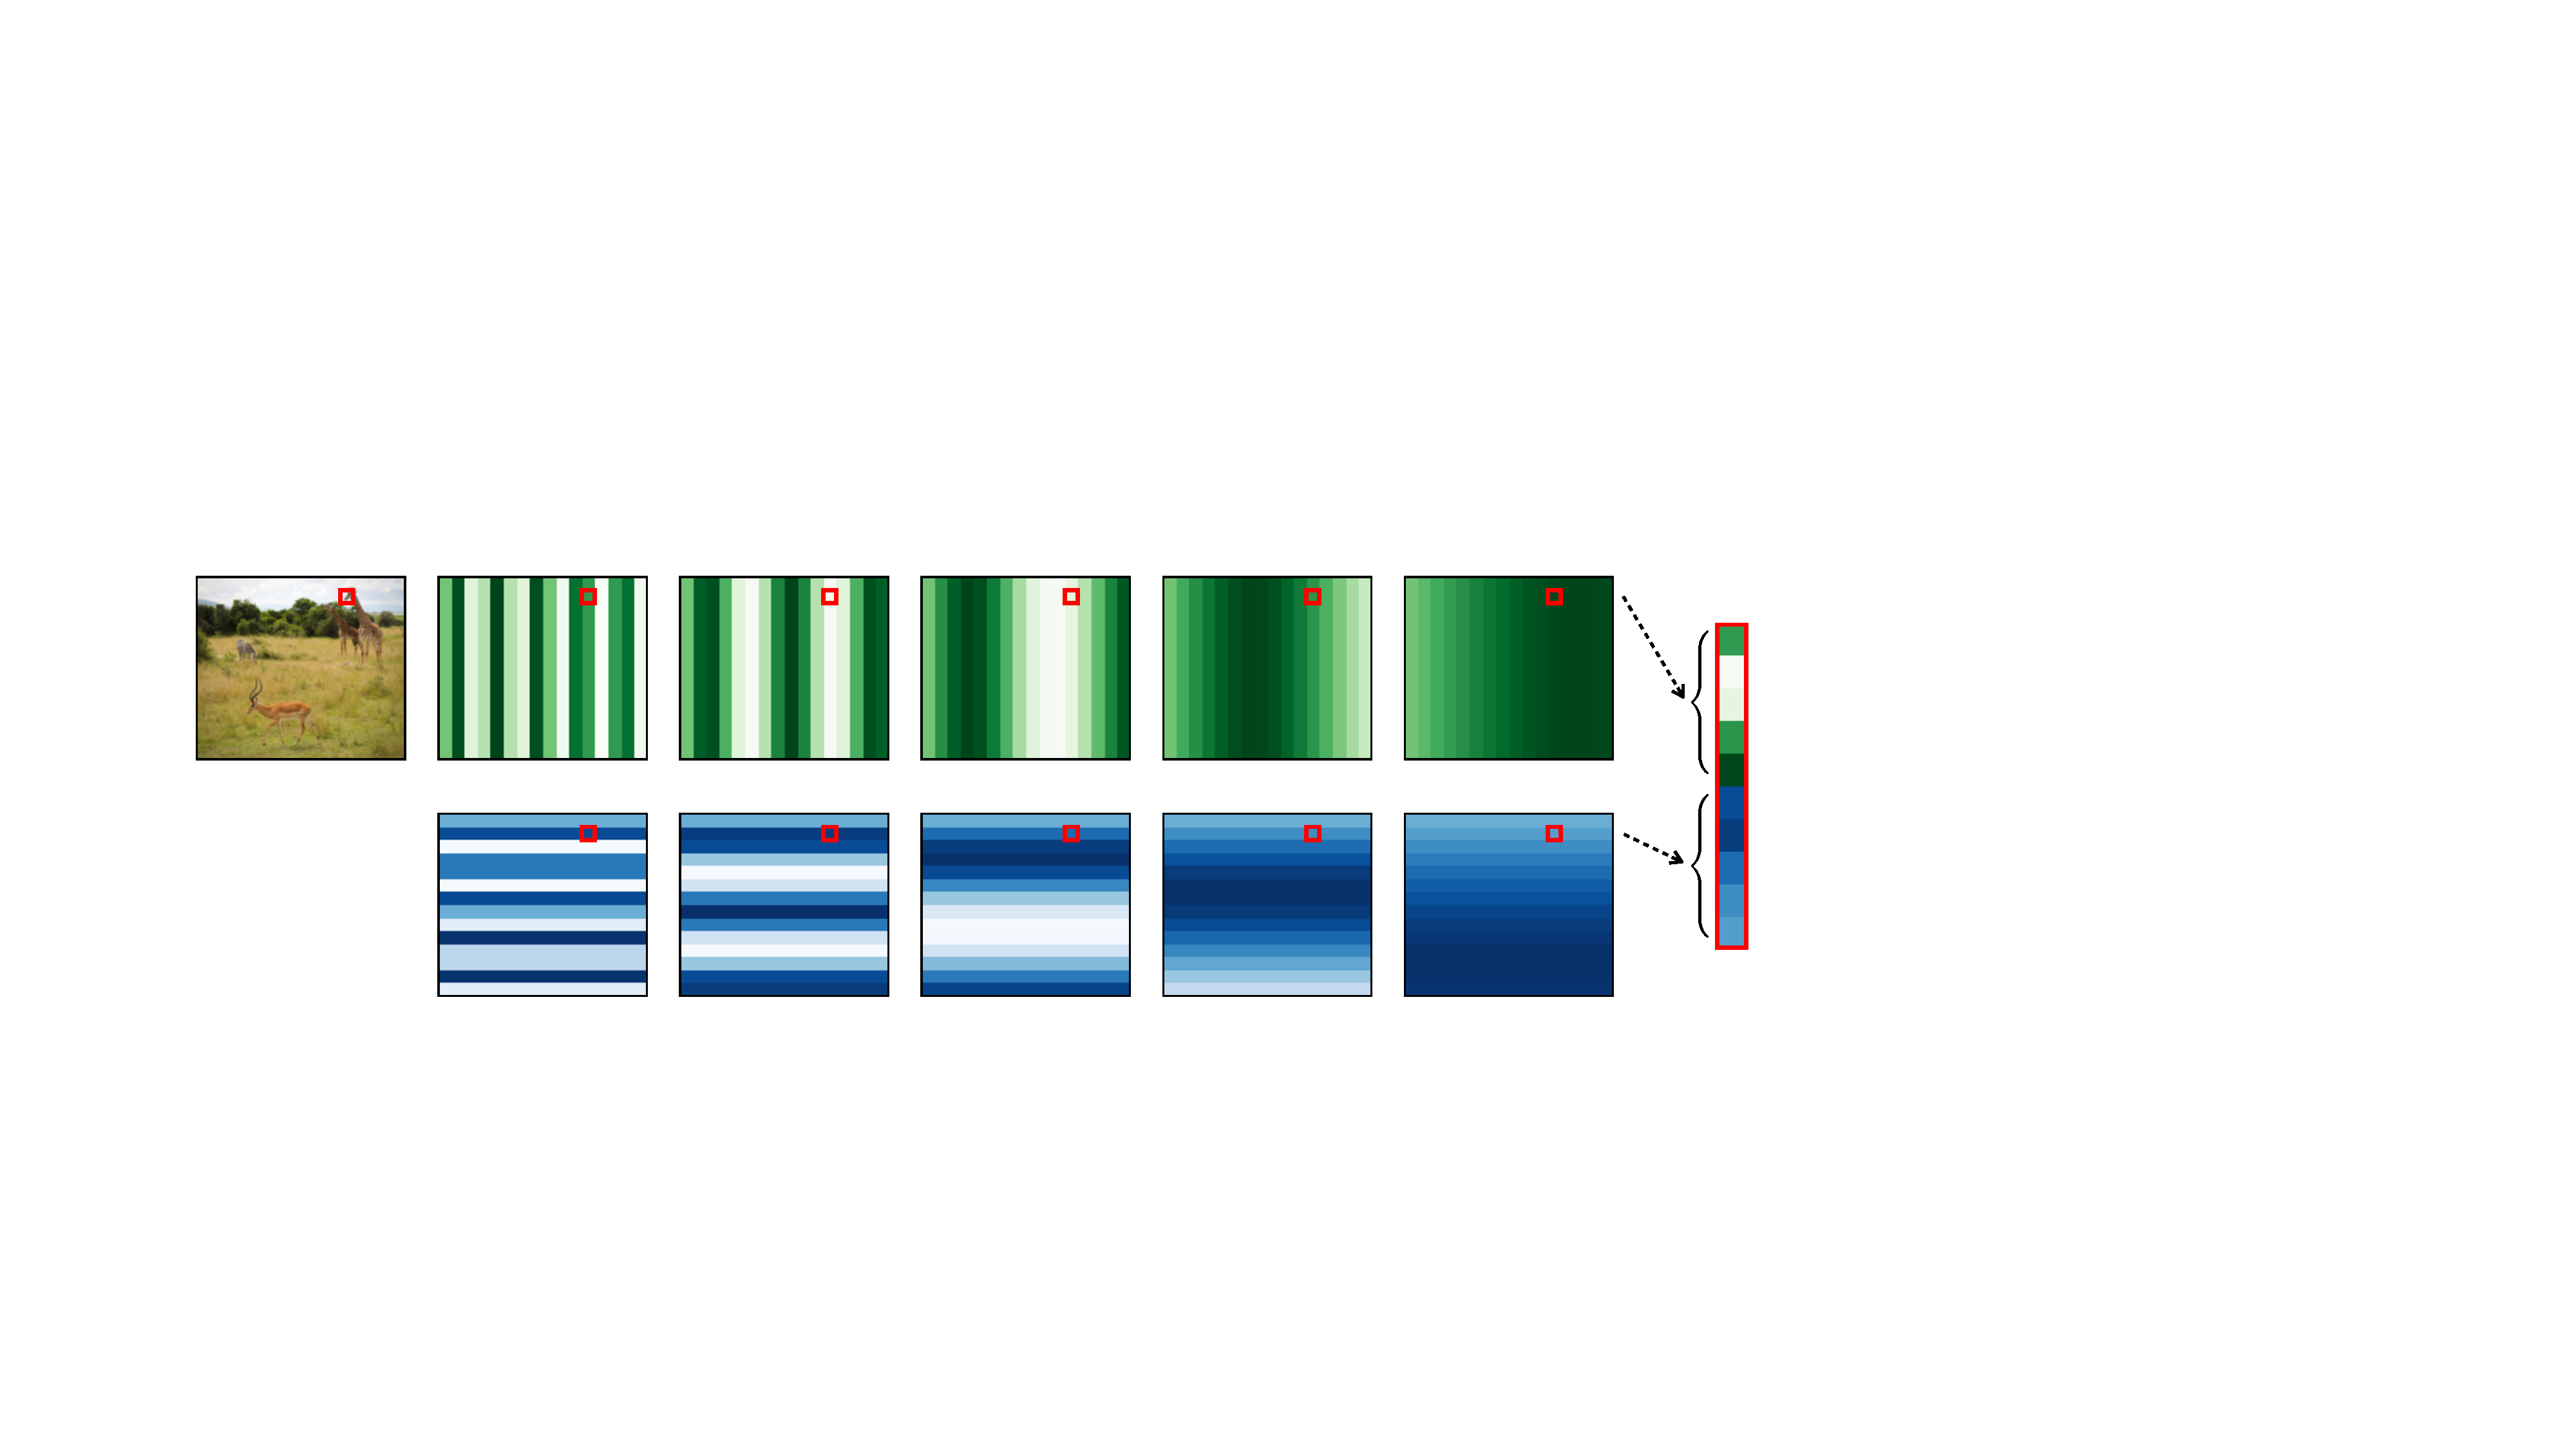
\includegraphics[width=1.0\linewidth]{./figures/transformers/positional_codes.pdf}};
            \draw (0, 2*\resy+\yoffset*3) node {\small{input}};
            \draw (\resx, 2*\resy+\yoffset*3) node {\small{$\sin(x)$}};
            \draw (2*\resx, 2*\resy+\yoffset*3) node {\small{$\sin(x/B)$}};
            \draw (3*\resx, 2*\resy+\yoffset*3) node {\small{$\sin(x/B^2)$}};
            \draw (4*\resx, 2*\resy+\yoffset*3) node {\small{$\sin(x/B^3)$}};
            \draw (5*\resx, 2*\resy+\yoffset*3) node {\small{$\sin(x/B^4)$}};
            %
            \draw (\resx, \resy+\yoffset) node {\small{$\sin(y)$}};
            \draw (2*\resx, \resy+\yoffset) node {\small{$\sin(y/B)$}};
            \draw (3*\resx, \resy+\yoffset) node {\small{$\sin(y/B^2)$}};
            \draw (4*\resx, \resy+\yoffset) node {\small{$\sin(y/B^3)$}};
            \draw (5*\resx, \resy+\yoffset) node {\small{$\sin(y/B^4)$}};
            %
            \draw (5.9*\resx, 2*\resy+0.15) node {\small{$\mathbf{p}$}};
        \end{tikzpicture}
    }
    \caption{Positional codes.}
    \label{fig:transformers:positional_codes}
\end{figure}

Another strategy is to simply let the positional codes be \textit{learned} by the model, which could potentially result in a better representation of space than sinusoidal codes~\cite{dosovitskiy2020vit}.

While positional encoding is useful and common in transformers, it is not specific to this architecture. The same kind of encodings can be useful for CNNs as well, as a way to make convolutional filters that are conditioned on position, thereby applying a different weighted sum at each location in the image~\cite{liu2018intriguing}. Positional encodings also appear in radiance fields, which we cover in \chap{\ref{chapter:nerfs}}. % for example, \cite{mildenhall2020nerf}.


% \section{Other uses of attention}

% It is also possible to attend between different sets of tokens, where queries produced by one set match with keys produced by a different set. Such a layer is simply called an {\bf attention layer} rather than a self-attention layer.

%A transformer is a CNN for which the filter weights are \textit{dynamic}. This means that the weights on each layer are not fixed during each forward pass but instead determined by the previous layer's activations.


\begin{figure}[t]
    \centerline{
        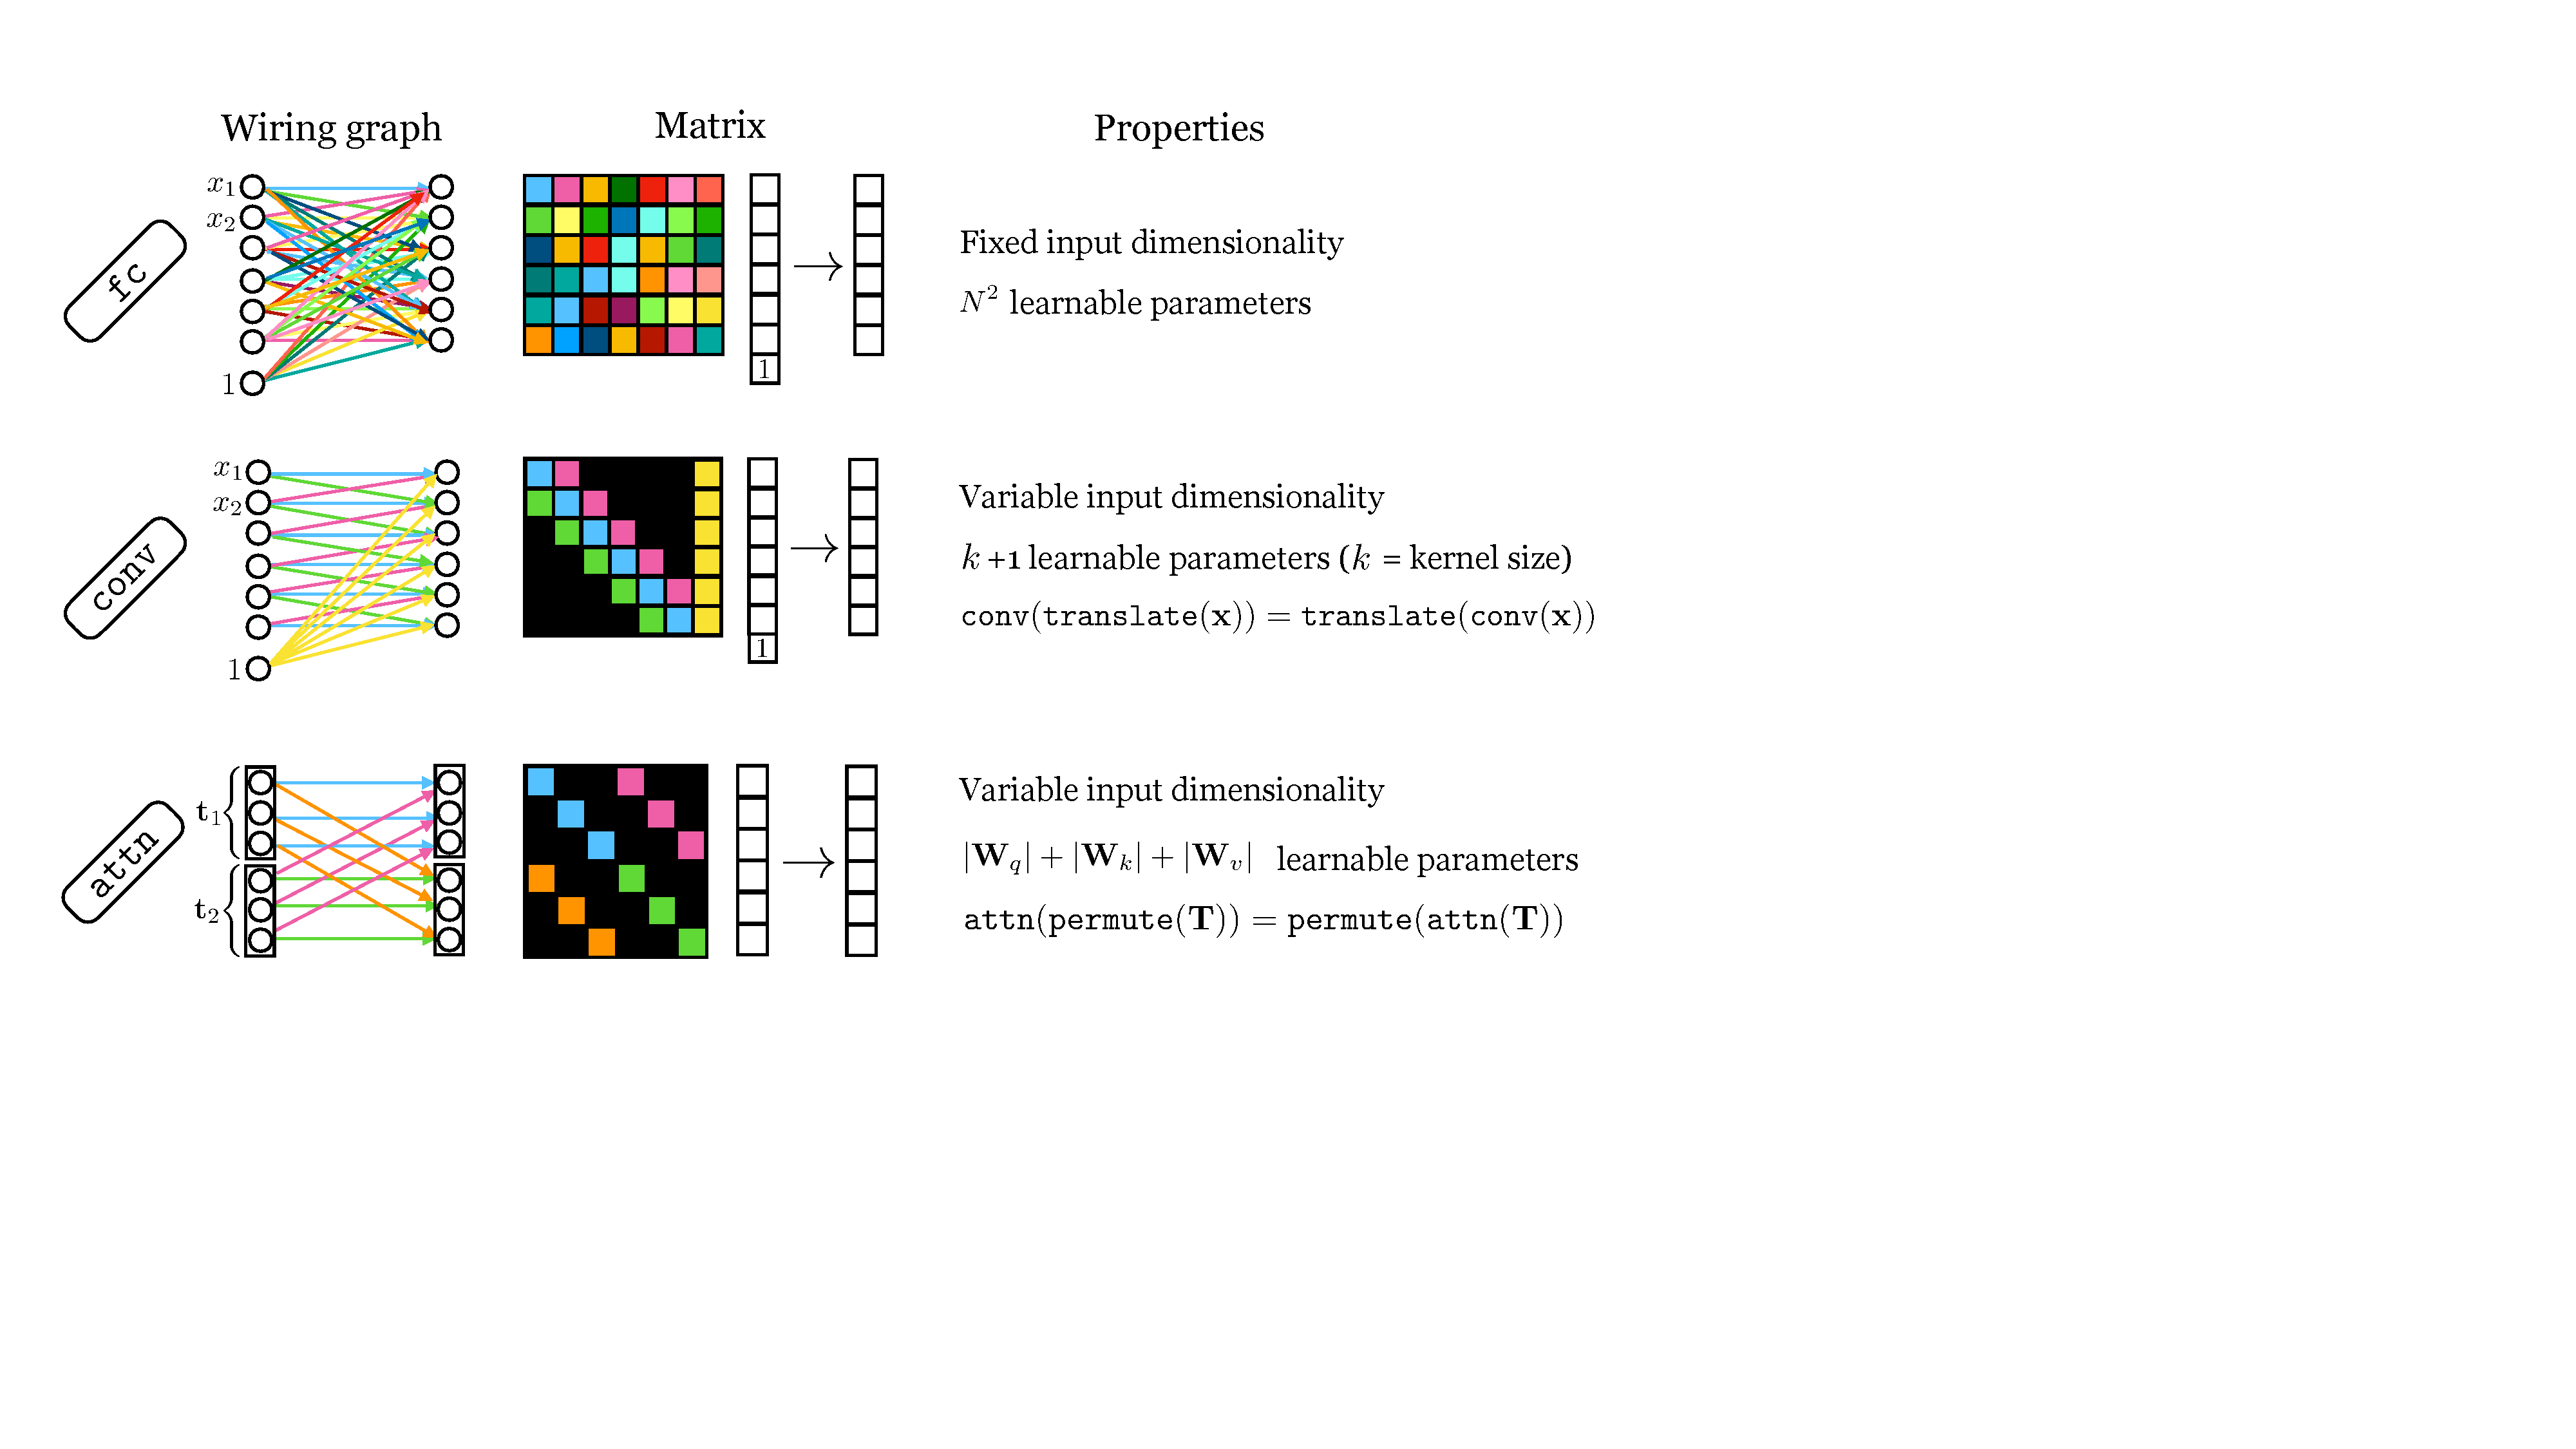
\includegraphics[width=1.0\linewidth]{figures/transformers/affine_layer_comparison.pdf}
    }
    \caption{Comparing different kinds of layers that all represent an affine transformation between the inputs and outputs.}
    \label{fig:transformers:affine_layer_comparison}
\end{figure}

\section{Comparing Fully Connected, Convolutional, and Self-Attention Layers}
\marginnote{The shorthand ``fc'' is often used to indicate a fully-connected linear layer.}
Many layers in deep nets are special kinds of affine transformations. Three we have seen so far are fully-connected layers (\texttt{fc}), convolutional layers (\texttt{conv}), and self-attention layers (\texttt{attn}). All these layers are alike in that their forward pass can be written as $\Xout = \mathbf{W}\Xin + \mathbf{b}$ for some matrix $\mathbf{W}$ and some vector $\mathbf{b}$. In \texttt{conv} and \texttt{attn} layers, $\mathbf{W}$ and $\mathbf{b}$ are determined as some function of the input $\Xin$. In \texttt{conv} layers this function is very simple: just make a Toeplitz matrix that repeats the convolutional kernel(s) to match the dimensionality of $\Xin$. In \texttt{attn} layers the function that determines $\mathbf{W}$ is a bit more involved, as we saw above, and typically we don't use biases $\mathbf{b}$.

Each of these layers can be represented as a matrix, and examining the structure in these matrices can be a useful way to understand their similarities and differences. The matrix for an \texttt{fc} layer is full rank, whereas the matrices for \texttt{conv} and \texttt{attn} layers have low-rank structure, but different kinds of low-rank structure. In \fig{\ref{fig:transformers:affine_layer_comparison}}, we show what these matrices look like, and also catalog some of the other important properties of each of these layers.


\section{Concluding Remarks}
As of this writing, transformers are the dominant architecture in computer vision and in fact in most fields of artificial intelligence. They combine many of the best ideas from earlier architectures—convolutional patchwise processing, residual connections, relu nonlinearities, and normalization layers—with several newer innovations, in particular, vector-valued tokens, attention layers, and positional codes. Transformers can also be considered as a special case of \textbf{graph neural networks} (\textbf{GNNs}). We do not have a separate chapter on GNNs in this book since GNNs, other than transformers, are not yet popular in computer vision. GNNs are a very general class of architecture for processing \textit{sets} by forming a graph of operations over the set. A transformer is doing exactly that: it takes an input set of tokens and, layer by layer, applies a network of transformations over that set until after enough layers a final representation or prediction is read out.